% A LaTeX template for MSc Thesis submissions to 
% Politecnico di Milano (PoliMi) - School of Industrial and Information Engineering
%
% S. Bonetti, A. Gruttadauria, G. Mescolini, A. Zingaro
% e-mail: template-tesi-ingind@polimi.it
%
% Last Revision: October 2021
%
% Copyright 2021 Politecnico di Milano, Italy. NC-BY

\documentclass{Configuration_Files/PoliMi3i_thesis}

%------------------------------------------------------------------------------
%	REQUIRED PACKAGES AND  CONFIGURATIONS
%------------------------------------------------------------------------------

% CONFIGURATIONS
\usepackage{parskip} % For paragraph layout
\usepackage{amssymb}
\usepackage{comment}
\usepackage{placeins}
\usepackage{csquotes}
\usepackage{setspace} % For using single or double spacing
\usepackage{emptypage} % To insert empty pages
\usepackage{multicol} % To write in multiple columns (executive summary)
\setlength\columnsep{15pt} % Column separation in executive summary
\setlength\parindent{0pt} % Indentation
\raggedbottom  

% PACKAGES FOR TITLES
\usepackage{titlesec}
% \titlespacing{\section}{left spacing}{before spacing}{after spacing}
\titlespacing{\section}{0pt}{3.3ex}{2ex}
\titlespacing{\subsection}{0pt}{3.3ex}{1.65ex}
\titlespacing{\subsubsection}{0pt}{3.3ex}{1ex}
\usepackage{color}

% PACKAGES FOR LANGUAGE AND FONT
\usepackage[english]{babel} % The document is in English  
\usepackage[utf8]{inputenc} % UTF8 encoding
\usepackage[T1]{fontenc} % Font encoding
\usepackage[11pt]{moresize} % Big fonts

% PACKAGES FOR IMAGES
\usepackage{graphicx}
\usepackage{transparent} % Enables transparent images
\usepackage{eso-pic} % For the background picture on the title page
\usepackage{subfig} % Numbered and caption subfigures using \subfloat.
\usepackage{tikz} % A package for high-quality hand-made figures.
\usetikzlibrary{}
\graphicspath{{./Images/}} % Directory of the images
\usepackage{caption} % Coloured captions
\usepackage{xcolor} % Coloured captions
\usepackage{amsthm,thmtools,xcolor} % Coloured "Theorem"
\usepackage{float}

% STANDARD MATH PACKAGES
\usepackage{amsmath}
\usepackage{amsthm}
\usepackage{amssymb}
\usepackage{amsfonts}
\usepackage{bm}
\usepackage[overload]{empheq} % For braced-style systems of equations.
\usepackage{fix-cm} % To override original LaTeX restrictions on sizes

% PACKAGES FOR TABLES
\usepackage{tabularx}
\usepackage{longtable} % Tables that can span several pages
\usepackage{colortbl}

% PACKAGES FOR ALGORITHMS (PSEUDO-CODE)
\usepackage{algorithm}
\usepackage{algorithmic}

% PACKAGES FOR REFERENCES & BIBLIOGRAPHY
\usepackage[colorlinks=true,linkcolor=black,anchorcolor=black,citecolor=black,filecolor=black,menucolor=black,runcolor=black,urlcolor=black]{hyperref} % Adds clickable links at references
\usepackage{cleveref}
\usepackage[square, numbers, sort&compress]{natbib} % Square brackets, citing references with numbers, citations sorted by appearance in the text and compressed
\bibliographystyle{abbrvnat} % You may use a different style adapted to your field

% OTHER PACKAGES
\usepackage{pdfpages} % To include a pdf file
\usepackage{afterpage}
\usepackage{lipsum} % DUMMY PACKAGE
\usepackage{fancyhdr} % For the headers
\fancyhf{}

% Input of configuration file. Do not change config.tex file unless you really know what you are doing. 
% Define blue color typical of polimi
\definecolor{bluepoli}{cmyk}{0.4,0.1,0,0.4}

% Custom theorem environments
\declaretheoremstyle[
  headfont=\color{bluepoli}\normalfont\bfseries,
  bodyfont=\color{black}\normalfont\itshape,
]{colored}

% Set-up caption colors
\captionsetup[figure]{labelfont={color=bluepoli}} % Set colour of the captions
\captionsetup[table]{labelfont={color=bluepoli}} % Set colour of the captions
\captionsetup[algorithm]{labelfont={color=bluepoli}} % Set colour of the captions

\theoremstyle{colored}
\newtheorem{theorem}{Theorem}[chapter]
\newtheorem{proposition}{Proposition}[chapter]

% Enhances the features of the standard "table" and "tabular" environments.
\newcommand\T{\rule{0pt}{2.6ex}}
\newcommand\B{\rule[-1.2ex]{0pt}{0pt}}

% Pseudo-code algorithm descriptions.
\newcounter{algsubstate}
\renewcommand{\thealgsubstate}{\alph{algsubstate}}
\newenvironment{algsubstates}
  {\setcounter{algsubstate}{0}%
   \renewcommand{\STATE}{%
     \stepcounter{algsubstate}%
     \Statex {\small\thealgsubstate:}\space}}
  {}

% New font size
\newcommand\numfontsize{\@setfontsize\Huge{200}{60}}

% Title format: chapter
\titleformat{\chapter}[hang]{
\fontsize{50}{20}\selectfont\bfseries\filright}{\textcolor{bluepoli} \thechapter\hsp\hspace{2mm}\textcolor{bluepoli}{|   }\hsp}{0pt}{\huge\bfseries \textcolor{bluepoli}
}

% Title format: section
\titleformat{\section}
{\color{bluepoli}\normalfont\Large\bfseries}
{\color{bluepoli}\thesection.}{1em}{}

% Title format: subsection
\titleformat{\subsection}
{\color{bluepoli}\normalfont\large\bfseries}
{\color{bluepoli}\thesubsection.}{1em}{}

% Title format: subsubsection
\titleformat{\subsubsection}
{\color{bluepoli}\normalfont\large\bfseries}
{\color{bluepoli}\thesubsubsection.}{1em}{}

% Shortening for setting no horizontal-spacing
\newcommand{\hsp}{\hspace{0pt}}

\makeatletter
% Renewcommand: cleardoublepage including the background pic
\renewcommand*\cleardoublepage{%
  \clearpage\if@twoside\ifodd\c@page\else
  \null
  \AddToShipoutPicture*{\BackgroundPic}
  \thispagestyle{empty}%
  \newpage
  \if@twocolumn\hbox{}\newpage\fi\fi\fi}
\makeatother

%For correctly numbering algorithms
\numberwithin{algorithm}{chapter}

%----------------------------------------------------------------------------
%	NEW COMMANDS DEFINED
%----------------------------------------------------------------------------

% EXAMPLES OF NEW COMMANDS
\newcommand{\bea}{\begin{eqnarray}} % Shortcut for equation arrays
\newcommand{\eea}{\end{eqnarray}}
\newcommand{\e}[1]{\times 10^{#1}}  % Powers of 10 notation

%----------------------------------------------------------------------------
%	ADD YOUR PACKAGES (be careful of package interaction)
%----------------------------------------------------------------------------

%----------------------------------------------------------------------------
%	ADD YOUR DEFINITIONS AND COMMANDS (be careful of existing commands)
%----------------------------------------------------------------------------

%----------------------------------------------------------------------------
%	BEGIN OF YOUR DOCUMENT
%----------------------------------------------------------------------------

\begin{document}

\fancypagestyle{plain}{%
\fancyhf{} % Clear all header and footer fields
\fancyhead[RO,RE]{\thepage} %RO=right odd, RE=right even
\renewcommand{\headrulewidth}{0pt}
\renewcommand{\footrulewidth}{0pt}}

%----------------------------------------------------------------------------
%	TITLE PAGE
%----------------------------------------------------------------------------

\pagestyle{empty} % No page numbers
\frontmatter % Use roman page numbering style (i, ii, iii, iv...) for the preamble pages

\puttitle{
	title=Conspiracy Theories vs Critical Thinking Using an Ensemble of Transformers and Large Language Models, % Title of the thesis
	name=Angelo Maximilian Tulbure, % Author Name and Surname
	course=Computer Science and Engineering - Ingegneria Informatica, % Study Programme (in Italian)
	ID  = 217764,  % Student ID number (numero di matricola)
	advisor= Prof. Mark James Carman, % Supervisor name
	coadvisor={Prof. Paolo Rosso, Mariona Coll Ardanuy (UPV)}, % Co-Supervisor name, remove this line if there is none
	academicyear={2023-24},  % Academic Year
} % These info will be put into your Title page 

%----------------------------------------------------------------------------
%	PREAMBLE PAGES: ABSTRACT (inglese e italiano), EXECUTIVE SUMMARY
%----------------------------------------------------------------------------
\startpreamble
\setcounter{page}{1} % Set page counter to 1

% ABSTRACT IN ENGLISH
\chapter*{Abstract}
This thesis contributes to the PAN at CLEF 2024 Oppositional Thinking Analysis shared task, focusing on automatically differentiating between conspiratorial and critical thinking narratives. The task includes binary classification to identify texts as conspiratorial or critical and span-level detection to recognize narrative elements like Agents, Facilitators, Victims, Campaigners, Objectives, and Negative Effects. Two multilingual datasets, in English and Spanish, with 5,000 annotated Telegram comments each, presented challenges such as class imbalances and complexities in detecting partially overlapping spans. 

For the binary classification task, a Soft Voting ensemble of fine-tuned Transformer models, enhanced with data augmentation techniques like back-translation, achieved F1-macro scores of 0.8917 for English and 0.8293 for Spanish.

The span-detection task emphasized precise tokenization and synonym replacement to maintain token alignment, crucial for detecting narrative spans. Great emphasis was placed on data preprocessing that further improved model robustness, achieving a span-F1 score of 0.6279 for English and 0.6129 for Spanish, which secured the best performance in the shared task for both languages and set a new state-of-the-art.

Additionally, experiments using Large Language Models (LLMs) significantly improved these results. By first employing zero-shot and few-shot learning techniques, and then fine-tuned LLMs enhanced cross-lingual understanding and narrative detection. These improvements underscore the effectiveness of LLMs in handling complex multilingual datasets, setting new performance benchmarks for both languages.

%This work demonstrates the potential of advanced NLP techniques to support misinformation detection and promote healthier public discourse online. 
This thesis contributes to the field of narrative analysis, offering insights that may inform future research on improving narrative detection across other domains and highlighting the role of automated systems in combating misinformation in digital spaces.
\\
\\
\textbf{Keywords:} oppositional thinking analysis, conspiracy theories, critical thinking, binary classification, span-level detection, transformers, LLMs, ensembling models % Keywords

% ABSTRACT IN ITALIAN
\chapter*{Abstract in lingua italiana}
La presente tesi contribuisce alla Oppositional Thinking Analysis shared task del PAN al CLEF 2024, concentrandosi sulla distinzione automatica tra narrazioni cospirazioniste e pensiero critico. Il task è suddiviso in una classificazione binaria per identificare i testi come cospirazionisti o critici e una rilevazione a livello di span per riconoscere elementi narrativi come Agenti, Facilitatori, Vittime, Attivisti, Obiettivi ed Effetti Negativi. Sono stati forniti due dataset multilingue, in inglese e spagnolo, ciascuno composto da 5.000 commenti annotati, che hanno presentato sfide come lo sbilanciamento delle classi e le complessità nella rilevazione di span parzialmente sovrapposti.

Per il task di classificazione binaria, un Soft Voting ensemble di fine-tuned Transformer models, potenziati con tecniche di aumento dei dati come la back-translation, ha ottenuto punteggi F1-macro pari a 0,8917 per l'inglese e 0,8293 per lo spagnolo.

Il task di rilevazione degli span ha enfatizzato la tokenizzazione precisa e la sostituzione tramite sinonimi per mantenere l’allineamento dei token, fondamentale per rilevare gli span narrativi. È stata posta grande enfasi sulla preelaborazione dei dati che ha ulteriormente migliorato la robustezza del modello, raggiungendo un punteggio span-F1 di 0,6279 per l’inglese e 0,6129 per lo spagnolo, garantendo i migliori risultati nel task per entrambe le lingue e stabilendo un nuovo riferimento per ricerche future. Inoltre, esperimenti con modelli di linguaggio di grandi dimensioni (LLM) hanno migliorato significativamente questi risultati. Utilizzando inizialmente tecniche di apprendimento zero-shot e few-shot, e successivamente facendo il fine-tuning dei LLM, è stata migliorata la comprensione interlinguistica e la rilevazione degli elementi narrativi. Questi miglioramenti evidenziano l'efficacia dei LLM nella gestione di dataset multilingue complessi, fissando nuovi standard di prestazione per entrambe le lingue. Questa tesi contribuisce al campo dell'analisi narrativa e sottolinea l'importanza dei sistemi automatizzati nella lotta alla disinformazione negli spazi digitali.
%Questo lavoro dimostra il potenziale delle tecniche avanzate di elaborazione del linguaggio naturale nel supportare la rilevazione della disinformazione e promuovere un discorso pubblico più sano online.
\\
\\
\textbf{Parole chiave:} analisi del pensiero oppositivo, teorie del complotto, pensiero critico, classificazione binaria, rilevamento a livello di span, transformers, LLMs, ensembling models % Keywords (italian)

%----------------------------------------------------------------------------
%	LIST OF CONTENTS/FIGURES/TABLES/SYMBOLS
%----------------------------------------------------------------------------

% TABLE OF CONTENTS
\thispagestyle{empty}
\tableofcontents % Table of contents 
\thispagestyle{empty}
\cleardoublepage

%-------------------------------------------------------------------------
%	THESIS MAIN TEXT
%-------------------------------------------------------------------------
% In the main text of your thesis you can write the chapters in two different ways:
%
%(1) As presented in this template you can write:
%    \chapter{Title of the chapter}
%    *body of the chapter*
%
%(2) You can write your chapter in a separated .tex file and then include it in the main file with the following command:
%    \chapter{Title of the chapter}
%    \input{chapter_file.tex}
%
% Especially for long thesis, we recommend you the second option.

\addtocontents{toc}{\vspace{2em}} % Add a gap in the Contents, for aesthetics
\mainmatter % Begin numeric (1,2,3...) page numbering

% --------------------------------------------------------------------------
% NUMBERED CHAPTERS % Regular chapters following
% --------------------------------------------------------------------------
\chapter{Introduction}
Conspiracy theories offer elaborate explanations for significant events, attributing them to hidden schemes orchestrated by secretive and powerful groups. On the other hand, critical thinking involves the careful evaluation of evidence, questioning assumptions, and forming reasoned judgments based on logical and evidence-based analysis. While both forms of thought may involve skepticism and questioning, they diverge in their goals and approaches. Critical thinking serves as a foundation for informed decision-making, challenging established norms through a structured examination of facts and reasoning. Conspiracy theories, instead, often rely on emotional appeal, selective use of evidence, and unverified claims, leading to distorted interpretations of reality. As a result, distinguishing between these two forms of thought is crucial for maintaining a healthy public discourse.

In today’s digital age, the rise of social media platforms has created an environment in which both conspiracy theories and critical perspectives can spread rapidly. Conspiracy theories, in particular, have flourished on social platforms, where the lack of fact-checking mechanisms and the speed of information sharing allow misinformation and disinformation to gain traction. While misinformation encompasses unintentional spreading of incorrect information, disinformation refers to false information deliberately spread with the intent to deceive. The consequences of this phenomenon can be severe, with widespread public confusion and erosion of trust in institutions. At the same time, social media platforms also serve as spaces for critical thinkers to question prevailing narratives and engage in constructive debate, which is essential for promoting transparency and accountability in society.

One of the main challenges in detecting conspiracy theories lies in their linguistic complexity and the rhetorical strategies they share with critical thinking. Both conspiracy theorists and critical thinkers question authority, present alternative viewpoints, and challenge mainstream narratives. However, while conspiracy theories often distort facts and rely on sensationalism, critical thinking is driven by logic and the pursuit of truth. This overlap in rhetorical style makes it difficult for automated systems to distinguish between the two, which can lead to the misclassification of critical thinking as conspiratorial or the failure to detect harmful misinformation. 

A crucial aspect of narrative detection, beyond the binary classification of conspiracy and critical thinking, is the identification of key elements that structure these narratives. These elements include Agents, who are portrayed as the primary actors responsible for certain actions or outcomes within a narrative. In conspiracy theories, agents are often characterized as powerful entities or organizations working in secret to manipulate events. Facilitators are individuals or groups that assist the agents in achieving their objectives, acting as intermediaries or supporters. Victims are those who suffer as a result of the agents’ actions, often depicted as the public or marginalized groups. Another essential element, Campaigners, are those who oppose the actions or narratives of the agents, frequently positioned as voices of resistance or opposition to the mainstream narrative. Objectives, in this context, represent the goals or intentions of the Agents, which in conspiracy narratives may involve the pursuit of political control, financial gain, or societal manipulation. Finally, negative effects refer to the adverse consequences experienced by the victims, which can range from public health crises to economic instability, depending on the narrative being propagated.

Recognizing these narrative elements is essential for understanding how both conspiracy theories and critical thinking are constructed and propagated. In many cases, the presence of these elements can be subtle, and they often overlap within a single narrative. For instance, a particular text might frame an individual as both a campaigner against the establishment and a victim of the actions taken by agents. This complexity poses additional challenges for automated systems, as distinguishing these elements within multilingual and cross-cultural contexts further complicates the detection process.

The shared task ``Oppositional thinking analysis: Conspiracy theories vs critical thinking narratives'' \cite{korencic2024oppositional}, part of PAN at CLEF 2024 \cite{bevendorff:2024}, addresses the problem of detecting these narratives in text. The task involves both binary classification, where texts are classified as either conspiratorial or critical, and span-level detection, where the narrative elements mentioned earlier must be identified and categorized. The dataset provided for this task consists of 5,000 annotated Telegram comments in English and other 5,000 in Spanish, which presents the additional challenge of handling multilingual data and the diverse narrative structures that come with it.

Our approach to these tasks involves fine-tuning transformer models, which have demonstrated state-of-the-art performance in natural language processing tasks \cite{tulbure2024conspiracy}. For the binary classification task, we employ a Soft Voting Ensembling method, which combines predictions from multiple transformer models to improve accuracy and robustness. The class imbalance present in the dataset, with a greater number of critical thinking texts compared to conspiracy texts, is addressed through data augmentation techniques, such as back-translation, which help to diversify the training data and reduce bias. 

For the span-level detection task, we treat the problem as a token classification task. This requires precise handling of tokenization and alignment to ensure that narrative spans are detected accurately. Given the presence of overlapping spans and the complexity of some texts, this task presents significant challenges. 

Due to our work, our team earned the distinction of being the best-performing team in the international Shared Task on Oppositional Thinking Analysis: Conspiracy Theories vs. Critical Thinking Narratives, as part of the PAN 2024 Lab of the CLEF Initiative\footnote{\url{https://pan.webis.de/clef24/pan24-web/oppositional-thinking-analysis.html\#award}} \cite{tulbure2024conspiracy}.

This research not only contributes to the technical advancements in narrative detection but also holds broader societal significance. The ability to accurately distinguish between conspiracy theories and critical thinking is essential for fostering constructive debate and preventing the spread of harmful misinformation. By identifying the key narrative elements that underpin these forms of thought, we can better understand how oppositional narratives are constructed and how they impact public discourse. This work ultimately aims to support efforts in promoting a more informed, critical, and healthy dialogue in digital spaces.

\section{Thesis Objectives}
The purpose of this thesis is to address the increasingly urgent need to differentiate between conspiracy theories and critical thinking in textual data, particularly in the context of online discussions where these narratives often overlap. This research contributes to the ongoing development of models and techniques that not only classify texts but also analyze the finer elements of oppositional narratives. Specifically, the thesis aims to:

\begin{itemize}
    \item Develop and fine-tune Transformer models to detect conspiracy theories and critical thinking narratives.
    \item Address the challenges posed by multilingual datasets, particularly in English and Spanish, focusing on improving performance across different languages and narrative structures.
    \item Implement span-level detection techniques that go beyond simple classification by identifying and categorizing key narrative elements.
    \item Explore the role of Large Language Models in enhancing narrative detection. 
    \item Incorporate techniques such as data augmentation to address class imbalance and improve model robustness.
    \item Provide insights into the broader implications of detecting oppositional narratives, highlighting the importance of these techniques in mitigating the spread of disinformation and promoting healthier public discourse in online environments.
\end{itemize}

This thesis provides a comprehensive framework for approaching the problem of oppositional thinking analysis and advances the state of the art in both binary classification and span-level detection of narratives. Concretely, we aim at answering the three following Research Questions (RQs):

\textbf{RQ1}. \textit{How effectively can transformer models and Large Language Models distinguish between conspiracy theories and critical thinking narratives, and which factors impact their performance?}

Subquestions:
\begin{itemize}
    \item \textit{What are the main challenges in differentiating linguistic and rhetorical features between conspiratorial and critical thinking narratives?}
    \item \textit{How do the performances of different models vary across languages?}
\end{itemize}
     
\textbf{RQ2}. \textit{How feasible is it to accurately identify text spans that correspond to key elements within oppositional narratives?}

Subquestions:
\begin{itemize}
\item \textit{What are the primary difficulties in detecting partially overlapping narrative elements in multilingual datasets?}
\item \textit{How does the context in which narrative elements appear influence their identification accuracy across different models?} 
\end{itemize}

\textbf{RQ3}. \textit{To what extent do data augmentation techniques enhance model performance across the two tasks?}

Subquestions:
\begin{itemize}
\item \textit{Which data augmentation techniques contribute most significantly to improving model performance in binary classification and span-level detection?}
\item \textit{How does data augmentation impact the model's ability to generalize across new or unseen narrative structures?}
\end{itemize}


\section{Structure of the Thesis}
The rest of the thesis is organised as follows:

Chapter \ref{chap:state_of_the_art}, \textit{State of the Art}, lays the foundational knowledge necessary for understanding the current methodologies and technological advancements in misinformation and disinformation detection. The evolution from traditional machine learning to modern deep learning, sets the stage for subsequent chapters.

Transitioning from these foundational concepts, Chapter \ref{chap:oppositional_thinking_tasks}, \textit{Evolution of Disinformation Detection Tasks}, traces the shift in focusing from profiling individuals who spread disinformation to a more nuanced analysis of the narratives themselves. This chapter enhances the discussion initiated in Chapter \ref{chap:state_of_the_art} by contextualizing the challenges and significance of the PAN 2024 challenge, bridging theoretical frameworks with practical research applications.

Following this contextual groundwork, Chapter \ref{chap:dataset_description}, \textit{Dataset Description}, introduces the datasets used in this study, focusing on their structure and the inherent challenges they pose, such as class imbalances and the complexities of narrative span detection. This detailed dataset description naturally leads into the practical applications and experimental setups discussed in the subsequent chapter.

Chapter \ref{chap:eval_metrics}, \textit{Evaluation Metrics}, outlines the metrics employed to assess model performance, providing a comprehensive foundation for understanding the empirical results discussed in later chapters. This section ensures that readers grasp the criteria used to evaluate the effectiveness of the models.

In Chapter \ref{chap:system_overview}, \textit{Experimental Framework}, the thesis transitions into a detailed discussion of the experimental setups used in the systems described in the following chapters.

Chapter \ref{chap:text_classification_task}, \textit{Binary Classification of Conspirational vs. Critical Thinking}, delves into the binary classification methodologies, discussing in-depth the processes of data processing, data augmentation, model training, and extraction of patterns. The integration and performance evaluation of various classifiers, especially ensemble methods, pave the way for a more granular analysis discussed in the following chapter.

Chapter \ref{chap:token_class_task}, \textit{Span-level Detection of Narrative Elements}, builds directly on the complexities introduced in Chapter \ref{chap:text_classification_task} by focusing on the token classification task. It provides an exhaustive analysis of the technical challenges encountered and the innovative solutions implemented to ensure precise token alignment and the effective handling of partially overlapping narrative elements.

Chapter \ref{chap:results_test_dataset}, \textit{Results on the Test Dataset}, presents the results of the models obtained on the test dataset. This chapter offers a critical evaluation of the effectiveness and limitations of the models across the two tasks.

Chapter \ref{chap:error_analysis}, \textit{Error Analysis}, reflects on the findings from Chapter 9 by conducting a detailed error analysis. This examination provides insights into the potential improvements and directs the focus toward future research paths discussed in the final chapter.

Chapter\ref{chap:experiments_LLMs_multilingual}, \textit{Experiments with LLMs and Multilingual Transformer Models}, explores the experiments conducted with Large Language Models (LLMs) and multilingual transformer models, assessing their performance across the two different languages and tasks. This chapter also includes a discussion on fine-tuning LLMs and adapting multilingual transformer models to tackle the challenges posed by narrative detection in both English and Spanish datasets.

Chapter \ref{chap:conclusion_future_work}, \textit{Conclusion and Future Work}, encapsulates the research findings, reflecting on the broader implications for narrative analysis and the field of disinformation detection. This chapter sets the stage for future work by outlining promising research trajectories based on the compiled research.

\textit{Appendices} offer additional methodological details and experimental results to bolster the transparency and reproducibility of the research.

%%%%%%%%%%%%%%%%%%%%%%%%%%%%%%%%%%%%%%%%%%%%%%%%%%%%%%%%%%%%%%%%%%%%%%%%%%%%%%%%%%%%%%%%%%%%%%%

\chapter{State of the Art} \label{chap:state_of_the_art}
This chapter introduces the state of the art in the field of disinformation and misinformation detection, outlining both the preliminary techniques and the most effective current methods, particularly in the areas of oppositional thinking analysis, focusing on binary classification and span-level detection.

\section{Disinformation vs Misinformation} \label{sec:disinformation_vs_misinformation}
In the digital era, the rapid spread of information has proven to be both a benefit and a challenge. While it enhances communication and broadens access to knowledge, it also accelerates the proliferation of false information. Among the most significant challenges are \textit{Disinformation} and \textit{Misinformation}, two related yet distinct concepts differentiated by their motivations and consequences. This section explores their definitions, impacts, and how they shape contemporary information ecosystems \cite{lazer2018science}.

%Disinformation 
Disinformation is the deliberate creation and distribution of false information with the intent to deceive and manipulate audiences. This orchestrated effort typically exploits vulnerabilities in belief systems by blending fact with fiction, making the falsehoods appear more credible \cite{ferrara2017disinformation}.

These campaigns often utilize sophisticated methods, including bots and trolls to amplify messages, fake news websites to create a facade of legitimacy, and social media algorithms to maximize dissemination. Targeted disinformation frequently preys on fears, biases, and uncertainties, making it an especially effective tool for dividing societies and eroding trust in institutions \cite{shao2017spread}.

One prominent example is the use of state-funded propaganda to manipulate public opinion, particularly during elections. Disinformation can skew perceptions of political candidates by spreading false narratives or damaging personal information, leading to manipulated voting outcomes. It also can foment social unrest by promoting divisive content aimed at weakening social cohesion and institutional trust \cite{allcott2017, bovet2019influence}.

A well-known case of disinformation is Russia’s interference in the 2016 U.S. presidential election, where the Internet Research Agency, a state-sponsored entity, systematically used fake accounts and misleading articles to manipulate public opinion \cite{mueller2019report}.

Disinformation’s impact extends beyond politics, infiltrating economic systems as well. False claims about companies or markets can cause volatility, affecting stock prices and financial stability. Moreover, the psychological phenomenon known as the "illusory truth effect" plays a significant role, where repeated exposure to false information can lead individuals to accept it as truth, further entrenching false beliefs and making corrective efforts difficult \cite{brennen2020types}.

%Misinformation 
Unlike disinformation, misinformation is not intended to deceive, but its consequences can be just as damaging, as it can perpetuate false beliefs, undermine trust in reliable sources, and contribute to the spread of unfounded claims or panic, much like disinformation does. \cite{lewandowsky2017beyond, guess2019}.

Social media platforms have made it easy for misinformation to spread rapidly through sharing and resharing, often without proper fact-checking. This is particularly concerning during crises, where uncertainty prevails. For example the rapid spread of misinformation on social media about virus transmission and preventive measures during the COVID-19 pandemic severely undermined public health efforts \cite{brennen2020types, who2020}.

Cognitive biases, such as confirmation bias, further accelerate the spread of misinformation. Individuals are more likely to accept information that aligns with their pre-existing beliefs, dismissing information that contradicts them. In like-minded communities, this reinforces the cycle of misinformation, allowing it to spread unchecked and creating echo chambers where falsehoods thrive \cite{cinelli2021echo, lazer2018science}.

The consequences of misinformation can be severe. In public health, for instance, misinformation about vaccines can lead to widespread vaccine hesitancy, which, in turn, undermines efforts to control preventable diseases. The spread of false information during health crises has shown how quickly misinformation can outpace authoritative responses, contributing to public confusion and the adoption of dangerous behaviors \cite{bursztyn2020misinformation}.

Addressing both disinformation and misinformation requires a multifaceted approach. For disinformation, regulatory measures are essential to hold platforms accountable, along with tools to detect and block disinformation campaigns before they spread. Increasing digital literacy among the public is equally critical, as it helps people recognize and resist false information.

Combatting misinformation, on the other hand, involves improving the transparency and accessibility of accurate information, especially during crises. Fact-checking services and tools can make a meaningful difference in mitigating the spread, but they must be accompanied by efforts to reduce cognitive biases and improve critical thinking skills across society \cite{mcgrew2017challenge, pennycook2019fighting}.

%%%%%%%%%%%%%%%%%%%%%%%%%%%%%%%%%%%%%%%%%%%%%%%%%%%%%%%%%%%%%%%%%%%%%%%%%%%%%%%%%%%%%%%%%%%

\section{Key Elements in Disinformation and Misinformation} \label{sec:key_elements_disinform_misinform}
In the context of disinformation and misinformation, understanding the various elements involved in false information campaigns is crucial. These elements shape the structure and impact of such campaigns, influencing how false information is created, propagated, and received. Key elements include:

\paragraph{Agents:} Individuals or groups who actively create and disseminate false information. In the case of disinformation, agents often include state actors, political operatives, or organized groups with a clear agenda to deceive and manipulate. These agents use sophisticated techniques to ensure their narratives reach and influence their target audience. For example, during the 2016 US presidential election, Russian operatives acting as agents created and distributed false information to sway public opinion. These agents used fake social media profiles and automated bots to amplify their messages, making them appear more credible and widely supported than they actually were \cite{bovet2019influence}.

\paragraph{Facilitators:} Those who assist agents in spreading false information. They may not be the originators  but play a significant role in its propagation. Facilitators can include media organizations, social media platforms, or individuals who share and amplify false narratives without necessarily understanding their falsehood or intent. For instance, during various misinformation campaigns, certain media outlets and social media users have unknowingly facilitated the spread of false information by sharing unverified reports and sensationalist stories \cite{marwick2017media}.

\paragraph{Victims:} Individuals or groups who are negatively affected by disinformation and misinformation. They may include the general public, specific communities, or even individual targets. Victims suffer the consequences of false information, which can range from confusion and mistrust to tangible harm. During the COVID-19 pandemic, victims of misinformation included individuals who, believing false information about the virus or vaccines, engaged in risky behaviors or avoided vaccination. This not only put their own health at risk but also contributed to broader public health challenges \cite{brennen2020types, vosoughi2018spread}.

\paragraph{Campaigners:} Individuals or groups who actively oppose the narratives pushed by mainstream sources or agents of disinformation. They work to challenge, debunk, or offer alternative perspectives to the dominant information streams. This opposition can involve activism, critical commentary, or advocacy for transparency and fact-checking. For instance, during various health crises, campaigners have played a vital role in challenging misinformation about diseases and their treatments by promoting evidence-based information and correcting public misconceptions. Their efforts are crucial in fostering a more informed public discourse and combating the effects of misinformation \cite{bevendorff:2024}.

\paragraph{Objectives:} Refer to the intentions of the agents behind disinformation campaigns. These can vary widely and include political gain, economic advantage, social disruption, or ideological influence. Understanding the objectives is crucial for developing strategies to counteract disinformation effectively. For example, during election periods, disinformation agents may aim to undermine confidence in the electoral process, discredit political opponents, or polarize the electorate to achieve specific political outcomes \cite{allcott2017, lazer2018science}.

\paragraph{Negative Effects:} Negative consequences suffered by the victims of disinformation and misinformation. These can include confusion, mistrust, social unrest, and tangible harm. The effects of disinformation can be far-reaching, impacting individuals, communities, and societal structures. In the context of public health, misinformation about medical treatments or preventive measures can lead to widespread harm. For instance, during the COVID-19 pandemic, the spread of misinformation about the virus, its transmission, and the vaccines contributed to confusion, fear, and poor health outcomes \cite{bursztyn2020misinformation}.

\paragraph{Amplifiers:} The mechanisms through which false information is spread more widely. This can include social media platforms, news outlets, or other communication channels that inadvertently or intentionally propagate disinformation or misinformation. They are essential in the virality of false information, as their reach and influence can exponentially increase the spread of inaccurate narratives. For example, algorithms on social media platforms that prioritize engaging content can inadvertently amplify disinformation, as sensationalist and misleading posts often receive more interactions and are thus more widely disseminated \cite{lazer2018science, cinelli2021echo}.

\paragraph{Correctors:} Individuals or organizations dedicated to identifying and debunking false information, such as fact-checking organizations, journalists, and informed citizens. Correctors work to provide accurate information, clarify misunderstandings, and reduce the impact of false narratives. During the COVID-19 pandemic, fact-checking organizations and public health authorities actively worked to debunk myths and provide accurate information about the virus and vaccines \cite{lazer2018science}.

\paragraph{Platforms:} Refer to the digital and physical spaces where information is shared and consumed. These include social media networks, news websites, and traditional media outlets. The policies and algorithms of these platforms significantly influence the spread of disinformation and misinformation. Social media platforms, for example, can either facilitate the rapid dissemination of false information through viral sharing mechanisms or help curb it by implementing stringent content moderation policies and promoting verified information sources \cite{gillespie2018custodians}.

\paragraph{Algorithms:} Systems used by social media platforms and search engines are instrumental in shaping the content users are exposed to. These mechanisms can unintentionally amplify disinformation and misinformation by favoring sensational, controversial, or highly engaging material, regardless of its factual accuracy. Efforts to address this issue focus on refining these systems to more effectively detect and downrank false information, while prioritizing verified and trustworthy sources \cite{gillespie2018custodians, shao2017spread}.

\paragraph{Bots and Trolls:} Automated or human-operated accounts used to amplify false information. Bots can generate and spread vast amounts of content quickly, creating the illusion of widespread support or belief in false narratives. Trolls, on the other hand, engage in disruptive behavior by posting inflammatory or off-topic messages to provoke and derail discussions. These entities are often employed in coordinated disinformation campaigns to increase the reach and impact of false information \cite{ferrara2017disinformation}.

In conclusion, understanding the various elements involved in information campaigns is essential for addressing the challenges posed by disinformation and misinformation. By identifying these key elements we can develop more effective strategies to combat the spread of false information. This comprehensive approach, combined with education, technological solutions, policy measures, and individual responsibility, can help protect the integrity of information in the digital age and foster a more informed and resilient society.

\section{Conspiracy Theory Detection} \label{sec:conspiracy_theory_detection}
Building on the discussion of disinformation and misinformation, conspiracy theories represent a potent subset of disinformation, characterized by false or unverified explanations for events, often attributing them to secret, malevolent groups or organizations. Their detection is critical for maintaining societal trust and cohesion \cite{douglas2023conspiracy}. On the other hand, critical thinking, rooted in academic discourse, challenge traditional power structures and ideologies but are sometimes misinterpreted as conspiracy theories when they question established narratives. Several techniques are used to identify conspiracy theories. Textual analysis remains one of the most prominent, focusing on key terminologies and narratives that reflect unsupported claims, often framed in emotionally charged language. Natural language processing (NLP) tools facilitate large-scale detection by analyzing these patterns across diverse online content \cite{marcellino2021detecting}.

Research has also explored psycho-linguistic traits to detect conspiracy theory propagators, analyzing factors like sentiment and rhetorical style \cite{giachanou2023detection}. For example, an analysis of Reddit revealed that while conspiracy theorists made up only 5\% of users, they were responsible for 64\% of the comments \cite{unesco2020}. Such patterns are useful in detecting individuals most likely to spread conspiratorial content. Taxonomies \cite{korenvcic2024distinguishes}, like Holour's classification of "insiders" versus "outsiders" \cite{holur2022insider}, further refine detection methods by highlighting in-group/out-group dynamics prevalent in conspiracy discourse. Emotional responses often differ between conspiracy and critical theory content. Conspiracy theories are more likely to evoke emotions like anger, disgust, or fear, while critical thinking may provoke reactions such as sadness or joy. Tools like Hurtlex\footnote{\url{https://github.com/valeriobasile/hurtlex}} help analyze these emotional cues, providing insights into the engagement strategies employed in conspiracy-laden content \cite{bassignana2018hurtlex}.

Automated fact-checking tools are invaluable for verifying claims and countering conspiracy theories. They cross-reference content with verified databases, flagging discrepancies in real-time \cite{graves2016deciding}. However, Brandolini’s law highlights the challenge of refuting false claims, which often requires more effort than creating them \cite{brandolini2013}. User behavior analysis complements these methods by examining interactions with content, such as likes, shares, and comments, to identify patterns typical of conspiracy theorists and their networks.

To differentiate between conspiracy and critical thinking, it's essential to recognize the academic rigor behind critical discourse. critical thinking are often published in scholarly journals and backed by research. Verifying their legitimacy involves cross-referencing with academic sources like JSTOR\footnote{\url{https://www.jstor.org}} or Google Scholar\footnote{\url{https://scholar.google.com}} \cite{souder2011ethics}. critical thinking also differ structurally and linguistically from conspiracy theories. It employs more complex academic language and methodological frameworks, supported by extensive references to scholarly work. Content analysis tools can help distinguish between these critiques and unsupported conspiracy narratives.

%%%%%%%%%%%%%%%%%%%%%%%%%%%%%%%%%%%%%%%%%%%%%%%%%%%%%%%%%%%%%%%%%%%%%%%%%%%%%%%%%%%%%%

\section{Binary Classification} \label{sec:binary_classification_task}
Having explored the landscape of disinformation and misinformation, along with the key elements involved in their dissemination, we now shift our focus to the computational techniques employed to detect and categorize such content. Among these, binary classification plays a fundamental role, particularly in distinguishing between categories like disinformation and reliable information, or between conspiracy and critical thinking narratives.

Binary classification is a specialized form of text classification, which involves assigning text documents to one of two predefined categories or labels. It plays a vital role in various applications, such as spam detection, sentiment analysis (positive vs. negative), and language identification \cite{jurafskyspeech}. By classifying large volumes of unstructured text into two meaningful categories, binary classification enables more efficient information retrieval and content management \cite{sebastiani2002machine}.

Historically, binary classification was performed manually by domain experts, such as doctors or auditors, who classified data based on established criteria or patterns \cite{jones1971makes}. However, manual classification was labor-intensive and prone to human error or subjectivity. Early attempts to automate binary classification in the 1960s and 1970s relied on rule-based systems, where classification was driven by manually created rules, such as using specific thresholds to detect fraud \cite{dale2000handbook}. While effective in some cases, these rule-based systems struggled with adaptability and required constant updates from experts whenever the data or classification criteria changed.

In the 1980s and 1990s, statistical approaches began to replace rule-based systems. Algorithms like Naive Bayes became popular due to their simplicity and relative effectiveness \cite{mitchell1997machine}. The development of techniques to represent data numerically, such as feature scaling and normalization, enhanced the performance of statistical models in binary classification. 

The late 1990s and early 2000s saw the introduction of machine learning algorithms, such as support vector machines (SVM) \cite{joachims1998text}, decision trees, and k-nearest neighbors (k-NN), which shifted the paradigm toward data-driven approaches. These algorithms allowed models to learn from data patterns rather than relying on fixed rules, marking a significant step toward scalable, automated binary classification.

By the 2010s, deep learning techniques emerged as a transformative force in binary classification. Unlike previous methods, deep learning models, especially convolutional neural networks (CNNs), recurrent neural networks (RNNs), and long short-term memory (LSTM) networks, automated the feature extraction process, learning representations of data that captured both local and sequential dependencies \cite{goodfellow2016deep}. The introduction of transformers \cite{wolf2020transformers}, a neural architecture based solely on self-attention mechanisms, further revolutionized binary classification by enabling models to process large amounts of data without the limitations inherent to RNNs \cite{vaswani2017attention}. Transformer-based models have set new benchmarks in classification tasks. Models like BERT \cite{devlin-etal-2019-bert}, GPT \cite{yenduri2024gpt}, RoBERTa \cite{Liu2019RoBERTaAR}, and T5 \cite{ni2022sentence} have been fine-tuned for specific binary classification tasks with remarkable efficiency \cite{wolf2020transformers}. These models have been evaluated on benchmarks such as the GLUE dataset \cite{wang2018glue}, achieving state-of-the-art results in tasks like sentiment analysis, natural language inference, and textual similarity.

%%%%%%%%%%%%% START ADDED %%%%%%%%%%%%%%%%%%%%%%
Large Language Models (LLMs), such as OpenAI’s GPT-4 \cite{aigpt}, Meta’s Llama 3 \cite{dubey2024llama}, and Google’s Gemini 1.5 \cite{team2023gemini}, have significantly advanced NLP by enabling sophisticated text understanding and generation. These models, trained on vast datasets, are commonly adapted for binary classification through fine-tuning and prompt engineering.

Fine-tuning tailors an LLM to a specific task by training it on labeled data, allowing it to capture task-relevant patterns while preserving its broad language capabilities. Studies have shown that fine-tuned LLMs frequently outperform traditional models on various binary classification benchmarks \cite{xiong2024fine}. For example, Llama 3.1 has demonstrated superior performance in sentiment analysis tasks \cite{myscale2024llama}.

Prompt-based methods, on the other hand, leverage zero and few-shot learning capabilities of LLMs by framing classification tasks as text generation challenges. Here, prompts guide the model to generate a response representing the classification label, making this approach effective in scenarios with limited labeled data, achieving competitive results on sentiment analysis and topic classification tasks \cite{liu2023pre}.

LLMs excel in tasks such as spam detection, fake news identification, and disinformation detection, leveraging contextual understanding to identify nuanced patterns. Their ability to detect complex patterns associated with disinformation and conspiracy theories makes them particularly suitable for these domains \cite{vykopal2023disinformation}. However, deploying LLMs for binary classification remains resource-intensive, often necessitating specialized hardware.
%%%%%%%%%%%%%% END ADDED %%%%%%%%%%%%%%%%

\subsection{Ensembling Models in Binary Classification} \label{subsec:ensembling_models_in_binary_class}
Ensembling in binary classification is an indispensable technique for enhancing model performance, particularly in addressing the challenges posed by the high dimensionality and variability of textual data. By combining the predictions of multiple models, ensembles can significantly improve both accuracy and generalization, making them a powerful tool in binary natural language processing tasks. This improvement stems from the ability of ensembles to aggregate the strengths of individual models, balancing out weaknesses and reducing the likelihood of overfitting to any particular aspect of the training data \cite{zhou2012ensemble}.

One common method in ensembling is Bagging (Bootstrap Aggregating), which trains multiple instances of the same model on different subsets of the training data, generated through bootstrapping. The individual models' predictions are then aggregated, typically via majority voting for binary classification tasks. Bagging reduces variance by ensuring that each model sees slightly different data, thereby leading to less correlated errors \cite{breiman1996bagging}. Random Forests, a popular extension of bagging applied to decision trees, have proven effective in binary classification by capturing a wide range of patterns from different perspectives within the data \cite{breiman2001random}. A visual representation of the process of Bagging can be seen in Figure \ref{ensemble_bagging}.

\begin{figure}[h!] 
\centering 
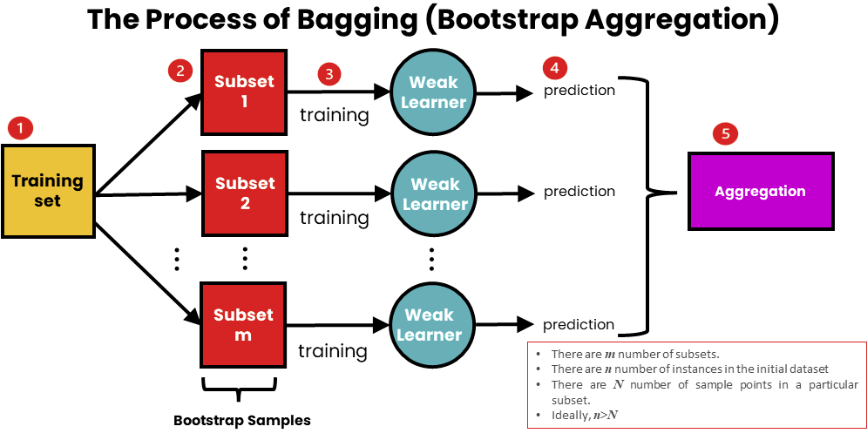
\includegraphics[width=0.78\linewidth, height=0.25\textheight]{Images/bagging.png} 
\caption{Process of Bagging: Boostrap Aggregation \cite{odegua2019empirical}} 
\label{ensemble_bagging} 
\end{figure} 
\FloatBarrier

Boosting (Figure \ref{ensemble_boosting}), in contrast to bagging, trains models sequentially, where each subsequent model focuses on correcting the errors made by the previous ones. This method emphasizes harder-to-classify instances, which makes boosting particularly adept at refining decision boundaries in noisy or complex datasets \cite{freund1997decision}. Algorithms like AdaBoost and Gradient Boosting Machines (GBM), including XGBoost \cite{chen2016xgboost} and LightGBM \cite{ke2017lightgbm}, are well-suited to binary classification tasks, where they excel at capturing intricate patterns in text data while being able to focus on difficult or borderline cases.

\begin{figure}[h!] 
\centering 
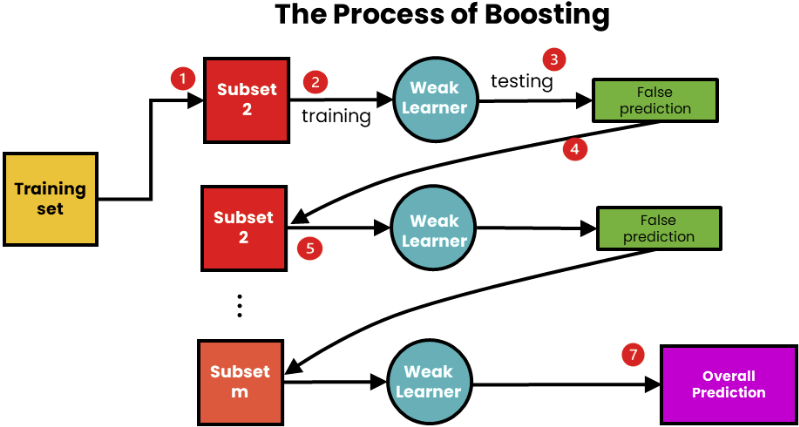
\includegraphics[width=0.73\linewidth, height=0.25\textheight]{Images/boosting.png} 
\caption{Process of Boosting \cite{odegua2019empirical}} 
\label{ensemble_boosting} 
\end{figure} 
\FloatBarrier

Stacking, (Figure \ref{ensemble_stacking}), is another advanced ensembling technique that combines predictions from several base models by training a meta-model to learn how to best integrate them \cite{wolpert1992stacked}. In binary classification, this allows for the combination of diverse models, such as logistic regression, support vector machines (SVMs), and neural networks, to build an ensemble that captures different facets of the data. The meta-model learns to weight the outputs of these base models, leveraging their individual strengths to create a more robust and accurate overall classifier \cite{zhou2012ensemble}.

\begin{figure}[h!] 
\centering 
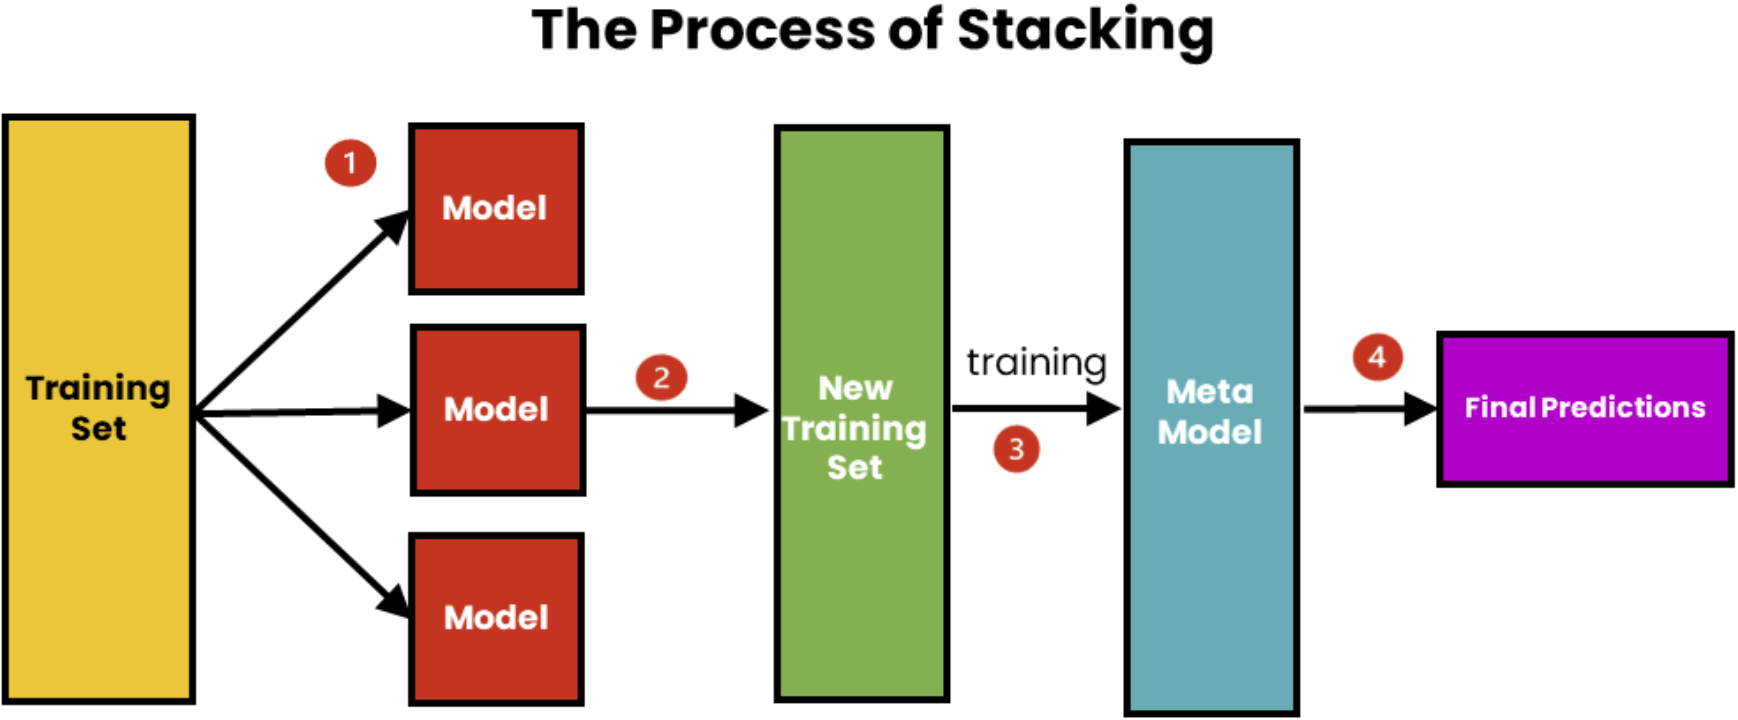
\includegraphics[width=0.75\linewidth, height=0.25\textheight]{Images/stacking.png} 
\caption{Process of Stacking \cite{odegua2019empirical}} 
\label{ensemble_stacking} 
\end{figure} 
\FloatBarrier

A more straightforward approach to ensembling in binary classification involves voting classifiers, which combine predictions through Hard or Soft voting. Hard voting, as depicted in Figure \ref{ensemble_hard_voting}, involves each base model casting a vote, with the final class being chosen based on the majority vote \cite{kuncheva2004combining}. This method works better when the individual classifiers are relatively accurate and diverse, as it relies on the majority of models being correct.

\begin{figure}[h!] 
\centering 
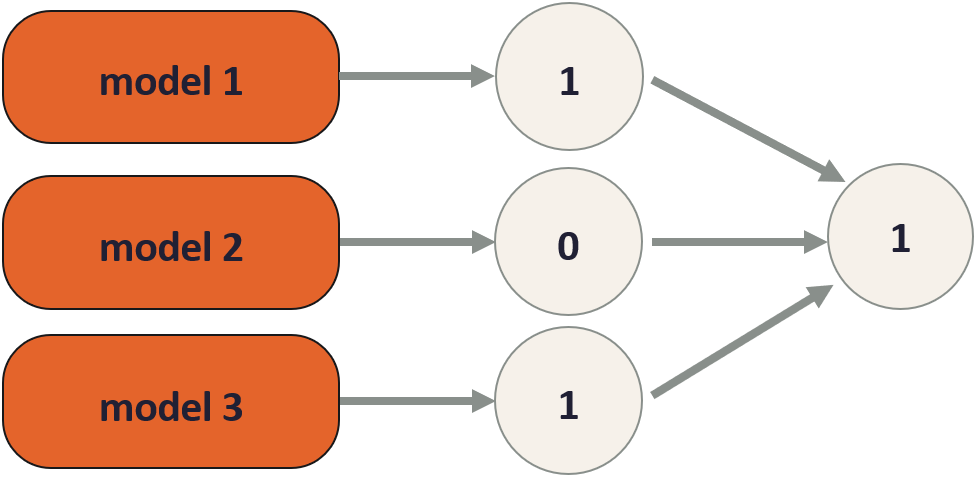
\includegraphics[width=0.64\linewidth, height=0.20\textheight]{Images/ensemble_hard_voting.png} 
\caption{Hard Voting Ensemble} 
\label{ensemble_hard_voting} 
\end{figure} 
\FloatBarrier

Soft voting, shown in Figure \ref{ensemble_soft_voting}, takes a more refined approach by averaging the predicted probabilities of each class across the models. This method often performs better than hard voting, as it accounts for the confidence of the base models' predictions, giving more weight to models that are more certain of their outputs \cite{zhou2012ensemble}.

\begin{figure}[h!] 
\centering 
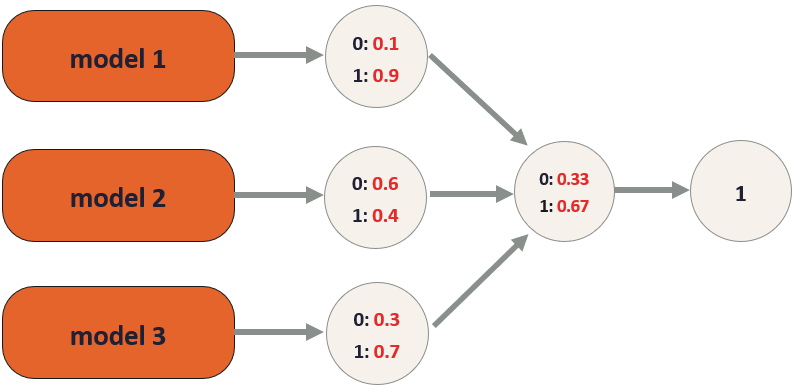
\includegraphics[width=0.73\linewidth, height=0.25\textheight]{Images/ensemble_soft_voting.png} 
\caption{Soft Voting Ensemble} 
\label{ensemble_soft_voting} 
\end{figure} 
\FloatBarrier

In practical terms, soft voting can be particularly useful in binary classification when base models vary significantly in their performance. Despite its successes, binary classification still faces several ongoing challenges. Data quality is a persistent issue, as high-quality labeled data is essential for training robust models, yet acquiring such data at scale can be difficult. Imbalanced datasets, where one of the two classes is underrepresented, can also bias models, making it harder to achieve accurate predictions for the minority class \cite{he2009learning}. Furthermore, deep learning models, particularly transformers, are often criticized for their lack of interpretability. As these models operate like “black boxes,” it is crucial to develop methods for explaining their decisions, especially in sensitive applications like healthcare or finance \cite{ribeiro2016trust}. Techniques like LIME \cite{ribeiro2016model} and SHAP \cite{lundberg2017unified} are being explored to provide more transparency. Real-time processing is another challenge, as the volume of data requiring classification grows exponentially. 

\section{Token Classification} \label{sec:token_classification}
While binary classification focuses on categorizing entire documents or instances into one of two predefined classes, token classification delves deeper by assigning labels to individual tokens, words, subwords, or characters, within a text sequence. This token-level labeling enables more granular extraction of structured information from unstructured text, which is critical for Natural Language Processing tasks that require understanding the roles of each token in context. Token classification powers a variety of advanced NLP applications, including Named Entity Recognition (NER) \cite{nadeau2007survey}, where entities such as names of people, organizations, or locations are identified; Part-of-Speech (POS) tagging \cite{toutanova2003feature}, which assigns grammatical categories to words; and chunking \cite{sang2000introduction}, where sequences of words are grouped into meaningful units like noun or verb phrases.

%As illustrated in Figure \ref{token_classification_overview}, 
Token classification provides a detailed view of text structure by labeling each token individually. This deeper level of analysis is crucial for more complex NLP tasks such as information retrieval \cite{jurafskyspeech}, question answering \cite{lample2016neural}, text summarization \cite{liu2019text}, and machine translation \cite{bahdanau2014neural}, where understanding the relationships between individual tokens and their contextual roles is predominant. For instance, NER, as shown in Figure \ref{ner_example}, is a core application of token classification. In this task, specific tokens like names of people, organizations, or dates are identified within a sentence, adding structure and meaning to otherwise unstructured data \cite{lample-etal-2016-neural}.

\begin{figure}[h!] 
\centering 
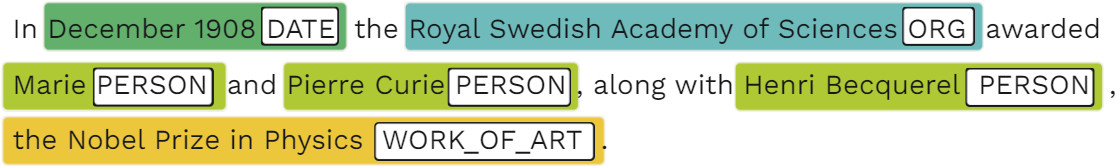
\includegraphics[width=0.85\linewidth,height=0.09\textheight]{Images/ner_example.png} 
\caption{Named Entity Recognition (NER) example} 
\label{ner_example} 
\end{figure} 
\FloatBarrier

Historically, early approaches to token classification relied on manually crafted linguistic rules to assign labels to tokens \cite{teller2000speech}. These systems, however, had limited generalizability and scalability. 

The shift to statistical models in the 1980s and 1990s marked a significant improvement. Methods such as Hidden Markov Models (HMMs) and Conditional Random Fields (CRFs) provided more robust solutions by modeling token relationships probabilistically. These models allowed systems to handle the ambiguity and variability of natural language more effectively, as they could capture dependencies between tokens \cite{rabiner1989tutorial, lafferty2001conditional}.

As machine learning gained prominence in the late 1990s and early 2000s, token classification evolved further with algorithms such as decision trees, Support Vector Machines, and maximum entropy models \cite{ratnaparkhi1996maximum}. However, these methods still relied heavily on manual feature engineering. Domain experts had to extract specific features from text, such as word frequencies or part-of-speech patterns, making the process labor-intensive.

The real breakthrough came in the 2010s with the rise of deep learning. Models like Recurrent Neural Networks (RNNs), Long Short-Term Memory (LSTM) networks, and later, transformers drastically changed token classification. 
These models automatically learned hierarchical representations of text and captured long-range dependencies between tokens, making them ideal for tasks such as NER, POS tagging, and chunking \cite{sherstinsky2020fundamentals}.

With the rise of deep learning, the success of token classification models depends not only on the architecture but also on the quality of the input text. Preprocessing, therefore, becomes a crucial step, as text needs to be prepared before it can be processed by machine learning models. This includes techniques like tokenization, which splits text into individual tokens; lemmatization, which reduces words to their root forms; and stop-word removal, which eliminates common but semantically insignificant words \cite{jurafskyspeech}. These preprocessing steps ensure that the input text is in a format suitable for analysis by token classification models. 

One of the most revolutionary advancements in token classification has been the development of transformer-based models. As shown in Figure \ref{transformers_self_attention}, transformers rely on self-attention mechanisms, allowing them to capture long-range dependencies between tokens more effectively than earlier methods like RNNs \cite{vaswani2017attention}. HuggingFace provides access to pre-trained transformer models like BERT \cite{devlin-etal-2019-bert}, GPT \cite{yenduri2024gpt}, RoBERTa \cite{Liu2019RoBERTaAR}, and T5 \cite{ni2022sentence}, which have dramatically transformed token classification by allowing users to fine-tune these models for specific tasks with minimal computational resources \cite{wolf2020transformers}. For example, BERT has achieved state-of-the-art results on the CoNLL-2003 NER dataset \cite{sang2003introduction}, demonstrating the model's ability to understand contextual relationships at the token level. RoBERTa and T5 have also been fine-tuned for various token classification tasks, consistently outperforming traditional models.

The key innovation that transformer models bring is transfer learning, which allows pre-trained models to be fine-tuned on task-specific datasets, significantly reducing the training time and amount of labeled data required. Because of that, transformer models can be adapted to token classification tasks with minimal labeled data. This has lowered the barrier to entry for deploying state-of-the-art token classification systems, allowing smaller organizations and even individual developers to leverage these advanced models. 
Additionally, multilingual models such as mBERT \cite{pires2019multilingual} and XLM-Roberta \cite{conneau2019unsupervised}, are extending token classification capabilities across multiple languages. These models enable NLP systems to function in diverse linguistic environments, expanding their applicability globally.

\begin{figure}[h!] 
\centering 
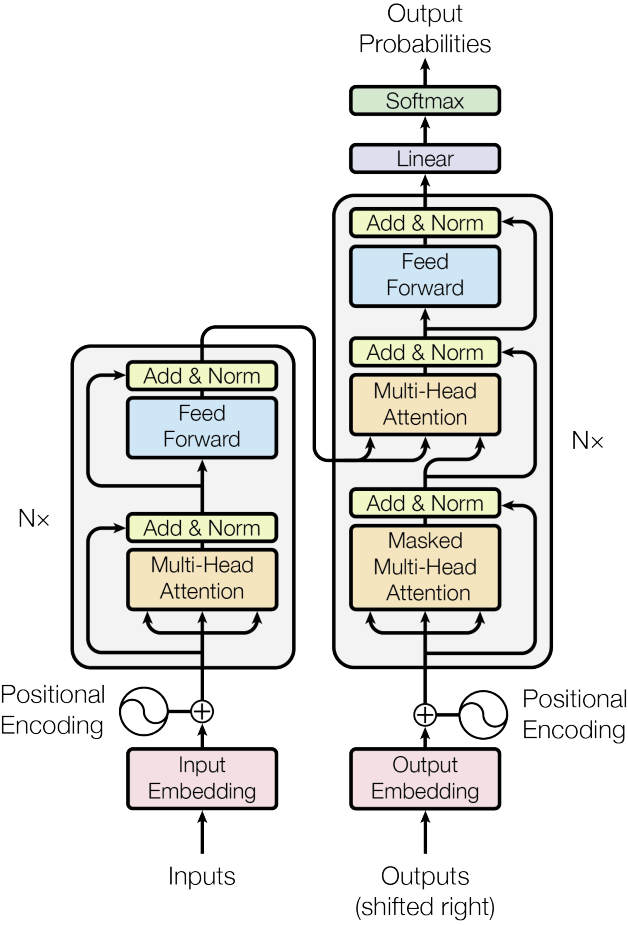
\includegraphics[width=0.48\linewidth, height=0.48\textheight]{Images/transformers_model.png} 
\caption{Transformer model architecture \cite{vaswani2017attention}} 
\label{transformers_self_attention} 
\end{figure} 
\FloatBarrier

%%%%%%%%%%%% START ADDED %%%%%%%%%%%%%%%%
Large Language Models have further advanced token classification by enabling models to understand complex linguistic patterns at the token level. LLMs have been adapted for token classification tasks using approaches like fine-tuning and prompt engineering.

Fine-tuning LLMs for token classification involves modifying the model architecture to produce token-level outputs. This is achieved by adding a token classification head to the model, allowing it to assign labels to individual tokens in the input sequence. %Studies have shown that fine-tuned LLMs achieve state-of-the-art results on NER and POS tagging tasks \cite{li2020dice}. For example, GPT-3, when fine-tuned, has demonstrated competitive performance on the CoNLL-2003 NER dataset, achieving high accuracy and F1 scores \cite{brown2020language}.

Prompt-based methods for token classification utilize the generative capabilities of LLMs by crafting prompts that elicit token-level outputs. For instance, prompting the model to generate annotations or labels for each token in a sentence. This approach has been explored in few-shot and zero-shot settings, demonstrating the flexibility of LLMs in adapting to token classification tasks without extensive labeled data \cite{grisanti2024named}.

%%%%%%%%%%%% END ADDED %%%%%%%%%%%%%%%%

\chapter{Evolution of Disinformation Detection Tasks} \label{chap:oppositional_thinking_tasks} The detection and analysis of disinformation and misinformation have evolved considerably in recent years, particularly as these phenomena have become more sophisticated and pervasive in digital media. Early research challenges, such as those presented in the \textit{PAN}\footnote{\url{https://pan.webis.de}} and \textit{MediaEval}\footnote{\url{https://multimediaeval.github.io}} series, primarily centered on profiling users and detecting false information at a broad level. However, the need to understand the structure of disinformation narratives, especially those that blur the line between legitimate criticism and conspiracy theories, has led to a shift in focus. The \textit{PAN 2024 Oppositional Thinking Analysis Challenge}\footnote{\url{https://pan.webis.de/clef24/pan24-web/oppositional-thinking-analysis.html}} exemplifies this shift by introducing more complex tasks that emphasize the detection of the components and structures that define oppositional narratives.

\section{The Evolution of Disinformation Detection Tasks} \label{sec:evolution_disinformation_detection_task} In the early stages of disinformation detection research, the primary goal was to identify users responsible for spreading fake news. The \textit{PAN 2020}\footnote{\url{https://pan.webis.de/clef20/pan20-web/author-profiling.html}} task Profiling Fake News Spreaders on Twitter \cite{rangel2020overview} was one of the pioneering efforts in this regard. It focused on profiling users by analyzing their linguistic and behavioral patterns to distinguish fake news spreaders from those sharing legitimate content. This task laid the groundwork for subsequent research by providing insights into how user behaviors could reveal patterns of disinformation dissemination.

%\section{Approaches in the MediaEval Series} \label{sec:multimodal_mediaeval} 
In parallel to \textit{PAN}, the \textit{MediaEval} series contributed significantly to advancing the detection of disinformation through tasks that analyzed both textual content and social network structures. The \textit{MediaEval 2020 Fake News: Corona Virus and 5G Conspiracy Multimedia Analysis Task}\footnote{\url{https://multimediaeval.github.io/editions/2020/tasks/fakenews/}} \cite{pogorelov2020fakenews} featured two primary subtasks: one focusing on natural language processing to classify tweets related to COVID-19 and 5G, and the other on structure-based analysis using Twitter network data. The dataset included two sets of tweets that mentioned the topics of Coronavirus and 5G, comprising text, reposting time patterns, and basic information about the users who reposted them. Additionally, the dataset provided a Twitter follower network, detailing the Twitter users who shared each respective tweet. This design emphasized the importance of combining linguistic features with reposting behaviors and network-based detection methods.

Subsequent editions, \textit{MediaEval 2021}\footnote{\url{https://multimediaeval.github.io/editions/2021/tasks/fakenews/}} and \textit{2022}\footnote{\url{https://multimediaeval.github.io/editions/2022/tasks/fakenews/}}, continued to emphasize the interplay between textual content and Twitter graph-based information for disinformation detection \cite{pogorelov2021fakenews, pogorelov2022fakenews}. These tasks underscored the necessity of understanding how disinformation narratives spread and evolve within social networks, focusing on the amplification of false content through structural and reposting patterns.

\section{The PAN 2024 Oppositional Thinking Challenge} \label{sec
} The \textit{PAN 2024 Oppositional Thinking Challenge} represents a significant leap forward in the analysis of disinformation by addressing the complexities of oppositional narratives. Moving beyond detecting false information or profiling fake news spreaders, the challenge introduces a more sophisticated set of tasks focused on the structure of narratives themselves. The challenge is divided into two subtasks: (i) Distinguishing between critical and conspiracy texts, and (ii) Detecting elements of the oppositional narratives.

\subsection{Binary Classification of Oppositional Narratives} \label{subsec
} The first task is a \textit{binary classification task}, where the goal is to classify a given text as either reflecting \textit{conspiratorial intent} or \textit{critical thinking}. This task addresses the challenge of distinguishing between two types of oppositional thought that, on the surface, can appear quite similar. Conspiratorial narratives often mimic the language and rhetorical strategies of critical thinking, using factual information mixed with distortions or falsehoods to create plausible but misleading arguments. Critical thinking, on the other hand, is characterized by a reasoned approach that challenges dominant narratives based on evidence and logical analysis.

\subsection{Detecting Elements of Oppositional Narratives} \label{subsec} The second task, \textit{detecting the elements of oppositional narratives}, is by far the most complex and significant aspect of the PAN 2024 challenge. Participants were required to identify and classify specific narrative elements within a text. These elements \cite{korenvcic2024distinguishes}, \textit{Agents}, \textit{Facilitators}, \textit{Victims}, \textit{Campaigners}, \textit{Objectives}, and \textit{Negative Effects}, are essential for understanding the deeper structure of how narratives are framed and presented.

\textbf{Agents} refer to the individuals or entities responsible for the actions or outcomes described in the narrative. \textbf{Facilitators} are those who assist the agents, enabling the events to unfold. \textbf{Victims} are the individuals or groups who suffer the consequences of the actions taken by the agents, while \textbf{Campaigners} represent those who oppose or resist the mainstream narrative or actions of the agents. \textbf{Objectives} outline the intentions or goals of the agents, and \textbf{Negative Effects} capture the consequences or harm caused by the events described.

The challenge of this task lies in the fact that these narrative elements are often embedded within one another, allowing for spans that encompass multiple roles. For example, a span-text discussing a \textit{Negative Effect} may include references to the \textit{Victim} affected by it. This overlapping nature requires an analysis approach that can detect and account for the fluid and nested relationships between these roles within oppositional narratives.

%\subsection{Challenges and Significance of Task 2} \label{subsec:significance_subtask2} 
This effort reflects the complexity of real-world disinformation and conspiracy theories. These narratives are often crafted to blur the lines between fact and fiction, and their effectiveness lies in their ability to weave multiple narrative elements together to create a compelling, although false, story. Understanding how these narratives are structured, and how different elements interact, is crucial for developing tools that can effectively combat disinformation.

This task also opens the door to more advanced forms of narrative analysis, such as understanding how different elements contribute to the overall persuasiveness of a narrative. By identifying patterns in the use of \textit{Agents}, \textit{Facilitators}, and the other elements, researchers can begin to map out common strategies used in conspiracy theories and in critical thinking. This could lead to more effective countermeasures, such as targeted fact-checking or interventions aimed at breaking down specific narrative structures.

%%%%%%%%%%%%%%%%%%%%%%%%%%%%% CHAPTER DATASET DESCRIPTION %%%%%%%%%%%%%%%%%%%%%%%%%%%%%%
\chapter{Dataset Description}  \label{chap:dataset_description}
In this chapter, we will analyze the dataset provided, examining its structure, the distribution of binary categories and the span-level annotations that highlight key elements within oppositional narratives.

\section{Dataset Overview and Binary Categories} \label{dataset_overview_and_binary_categories}
For this task, the organisers provided a JSON file containing all texts in the training dataset along with their annotations. Each text is represented by a dictionary that includes the ID, tokenized text, binary category, and span annotations with their categories. Span annotations are provided as a list of dictionaries, with each dictionary representing an annotated span and detailing the span's category and text, specified by the start and end characters. The training dataset, comprising 4000 records extracted from Telegram comments, was released with all annotations, while the test dataset, consisting of 1000 records, was released only with ``id'' and the ``text'' field~\cite{korencic2024oppositional,bevendorff:2024}.

\begin{figure}[H]
    \centering
    \subfloat[Binary categories for the English dataset\label{fig:distr_binary_en}]{
        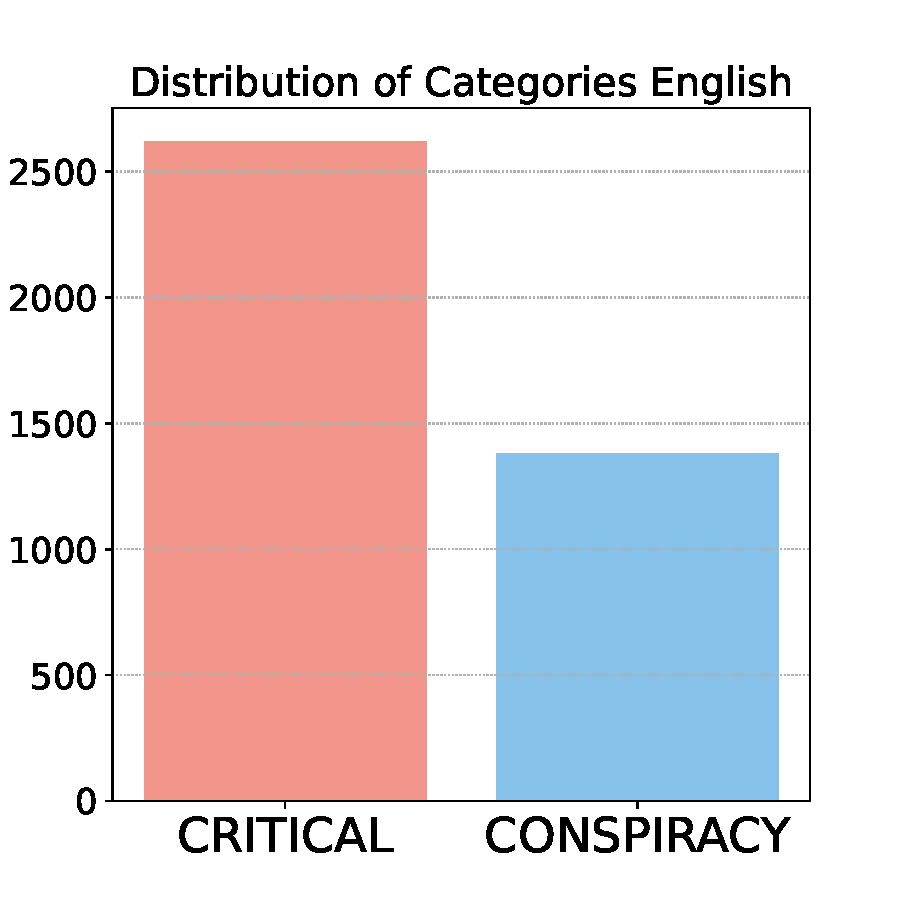
\includegraphics[scale=0.48]{Images/category_count_t1_en_v2.pdf}
    }
    \quad
    \subfloat[binary categories for the Spanish dataset\label{fig:distr_binary_es}]{
        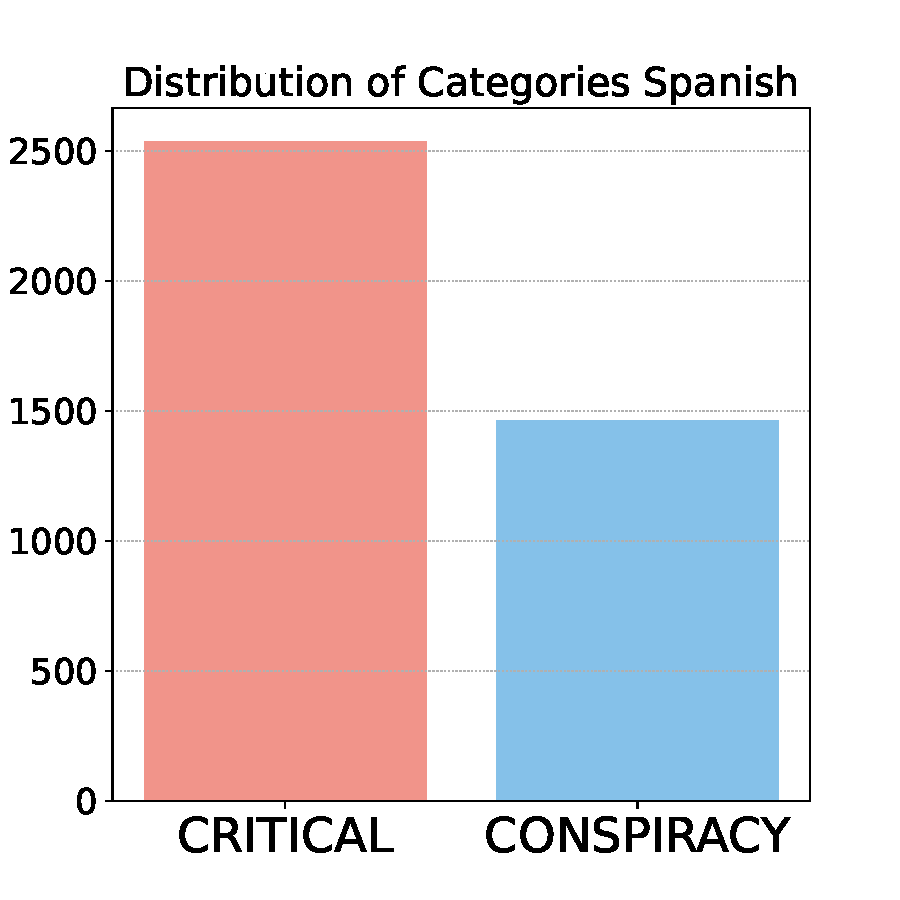
\includegraphics[scale=0.48]{Images/category_count_t1_es_v2.pdf}
    }
    \caption{Distribution of binary categories for English and Spanish train datasets}
    \label{fig:test}
\end{figure}

\begin{table}[H]
    \centering
    %\small
    %\begin{tabular}{lrrrr}
    \begin{tabular}{lcccc}
        \hline
        \textbf{Label} & \textbf{English} & \textbf{(\%)} & \textbf{Spanish} & \textbf{(\%)} \\
        \hline
        CRITICAL     & 2621 & 65.53\% & 2538 & 63.45\% \\
        CONSPIRACY   & 1379 & 34.48\% & 1462 & 36.55\% \\
        \hline
    \end{tabular}
    \caption{\small Distribution of binary labels for the English and Spanish train datasets}
    \label{tab:label_distribution_1}
\end{table}



\noindent As summarized in Table \ref{tab:label_distribution_1} and shown in Figures \ref{fig:distr_binary_en} and \ref{fig:distr_binary_es}, the binary classification task for distinguishing critical from conspiracy texts reveals an inherent class imbalance in both the English and Spanish datasets. The English dataset has 65.53\% critical texts compared to 34.48\% conspiracy texts, while the Spanish dataset shows a similar trend with 63.45\% critical and 36.55\% conspiracy texts. This imbalance poses a significant challenge for model training, as models may become biased towards the more frequent class (critical texts), potentially overlooking subtle features of conspiracy texts.
The similarity in the proportions of critical and conspiracy texts across both languages suggested that the models trained on one dataset might be adaptable to the other with minimal adjustments. That was indeed the approach that we adopted for the shared task. Examples for each category are shown in Table \ref{tab:example_binary_task_critical_text} and in Table \ref{tab:example_binary_task_conspiracy_text}.

\begin{table}[h]
    \centering
    \renewcommand{\arraystretch}{1.5} 
    \begin{tabular}{p{12cm}c}
        \hline
        \textbf{Text} & \textbf{Category} \\
        \hline
        CNN continued its wall to wall broadcasts calling for unvaccinated people to be punished, with analysts again calling for those who have not gotten the COVID shots to be segregated from society and forced to pay for tests every single day. https://summit.news/2021/07/23/cnn ... /
        & CRITICAL \\
        \hline
        Are women suffering adverse injuries and deaths from the Covid - 19 vaccinations in far greater numbers than men? Data from the EU suggests that this is indeed the case with women reporting more than three times the issues that men are. This data is not provided by the MHRA in the UK but you can access the EU data here by vaccine manufacturer https:// expose - news .com/2022/06/08/ ...
        & CRITICAL \\
        \hline
        Joe Biden's Commerce Secretary has claimed that nobody is being forced to get vaccinated, despite last week's announcement that millions of Americans will be mandated to take the shot in order to go to work . https :// summit . news / 2021 / 09 / 15 / ...
        & CRITICAL \\
        \hline
    \end{tabular}
    \caption{\small Examples of critical texts}
    \label{tab:example_binary_task_critical_text}
\end{table}
\FloatBarrier

\begin{table}[h]
    \centering
    \renewcommand{\arraystretch}{1.5} 
    \begin{tabular}{p{12cm}c}
        \hline
        \textbf{Text} & \textbf{Category} \\
        \hline
        Agenda 21 ... Goal 1: End poverty in all its forms everywhere Translation: Centralized banks, IMF, World Bank, Fed to control all finances , digital one world currency in a cashless society Goal 2: End hunger, achieve food security: GMO Goal 3: Ensure healthy lives and promote well - being for all at all ages Translation: Mass vaccination, Codex Alimentarius ... Population control through forced “Family Planning” ... & CONSPIRACY \\
        \hline
        THE NEW WORLD ORDER JUST PUSHED THE TURBO BUTTON - - WHO STILL THINKS IT'S A CONSPIRACY THEORY? Think back to WWII. This is the same thing. They cause a big global crisis to enact their agenda through treaties and create hegemony. Why people can not see this as the same playbook is just mind blowing to me. All wars are literally cover for these agendas. Covid is WWIII without the guns and bombs.  https://www.dailymail.co.uk/ ... @DismantlingTheCabal  & CONSPIRACY \\
        \hline
        PfizerGate Scandal: The Worldwide Cover-up of Data to disguise the fact Covid-19 Vaccines cause VAIDS. Health authorities around the world are manipulating figures in an attempt to hide from the general public that the Covid-19 injections are causing the fully vaccinated to develop Vaccine Acquired Immune Deficiency Syndrome; and we can prove it … & CONSPIRACY \\
        \hline
    \end{tabular}
    \caption{\small  Examples of conspiracy texts}
    \label{tab:example_binary_task_conspiracy_text}
\end{table}
\FloatBarrier

\section{Span-Level Annotations and Analysis} \label{sec:span_level_annotations_analysis}
Apart from the binary label, the messages also include annotated token-level elements. According to the dataset's authors \cite{korenvcic2024distinguishes}, these elements represent "the key elements of oppositional narratives." The six span categories defined by the authors of the PAN task are:

\begin{itemize}
    \item \textbf{Agents}: Individuals or entities responsible for the actions and/or negative effects.
    \item \textbf{Facilitators}: Those who assist the agents.
    \item \textbf{Victims}: Those who suffer the consequences of the agents' actions.
    \item \textbf{Campaigners}: Those who oppose the mainstream narrative.
    \item \textbf{Objectives}: The goals or intentions of the agents.
    \item \textbf{Negative effects}: The adverse consequences experienced by the victims.
\end{itemize}

Table \ref{tab:example_span_text} shows that a single text message can contain multiple span elements of the same category. It is also important to note that some texts may not contain any span elements. Additionally the span text can partially overlap and this increases exponentially the difficulty in finding all the span elements.

\begin{table}[H]
    \centering
    \small
    \renewcommand{\arraystretch}{1.6} % Adjust the value to increase the space between lines
    \begin{tabular}{p{12cm}c}
        \hline
        \textbf{Span Text} & \textbf{Category} \\
        \hline
        Joe Biden's Commerce Secretary & AGENT \\
        THE NEW WORLD ORDER & AGENT \\
        vaccine manufacturer & AGENT \\
        \hline
        analysts & FACILITATOR \\
        CNN & FACILITATOR \\
        Health authorities around the world & FACILITATOR \\
        \hline
        millions of Americans & VICTIM \\
        unvaccinated people & VICTIM \\
        women & VICTIM \\
        \hline
        summit & CAMPAIGNER \\
        expose-news & CAMPAIGNER \\
        DismantlingTheCabal & CAMPAIGNER \\
        \hline
        Centralized banks, IMF, World Bank, Fed to control all finances, digital one world currency in a cashless society & OBJECTIVE \\
        Mass vaccination, Codex Alimentarius Goal & OBJECTIVE \\
        Population control through forced "Family Planning" & OBJECTIVE \\
        \hline
        the fact Covid - 19 Vaccines cause VAIDS & NEGATIVE\_EFFECT \\
        women reporting more than three times the issues that men are & NEGATIVE\_EFFECT \\
        adverse injuries and deaths from the Covid - 19 vaccinations & NEGATIVE\_EFFECT \\
        \hline
    \end{tabular}
    \caption{Span elements from the critical texts in Table \ref{tab:example_binary_task_critical_text} and from the conspiracy texts in Table \ref{tab:example_binary_task_conspiracy_text} used for the span-level detection task}
    \label{tab:example_span_text}
\end{table}
\FloatBarrier

%%%%%%%%%%%%%%%%%%%% START new part %%%%%%%%%%%%%%%%%%%%%%%
In order to better understand the structure of the oppositional narratives scheme, a visual example can be found in Figure \ref{fig:critical_conspiracy_annotation}. 
In Figure \ref{fig:critical_thinking_annotation} we can observe a critical thinking message  annotated with the six different categories, while in Figure \ref{fig:conspiracy_theory_annotation} we can observe a conspiracy theory message.

\begin{figure}[h]
    \centering
    \subfloat[A critical message annotated with elements of oppositional narrative \label{fig:critical_thinking_annotation}]{
        %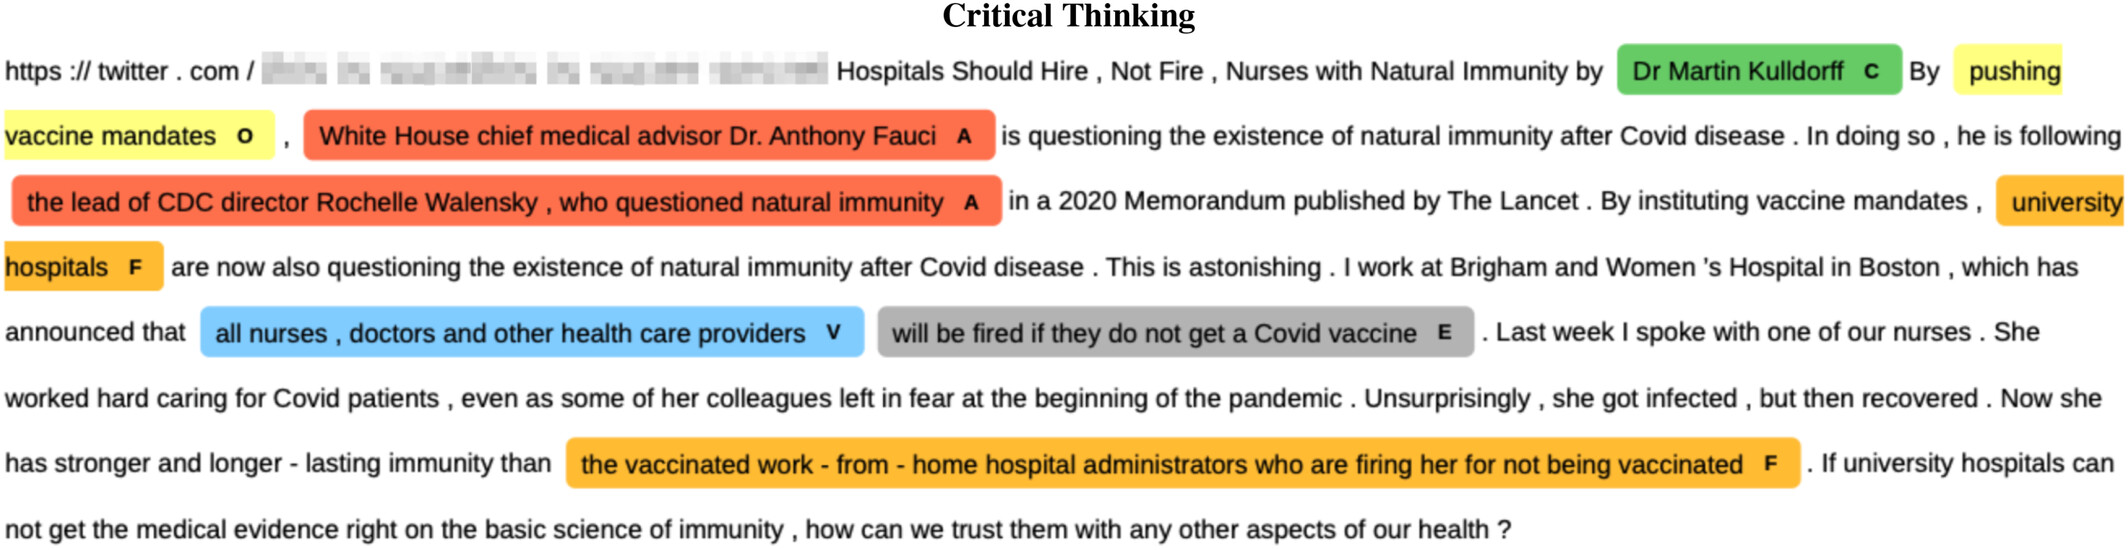
\includegraphics[width=1\textwidth, height=0.25\textheight]{Images/critical_thinking_annotation.png}
        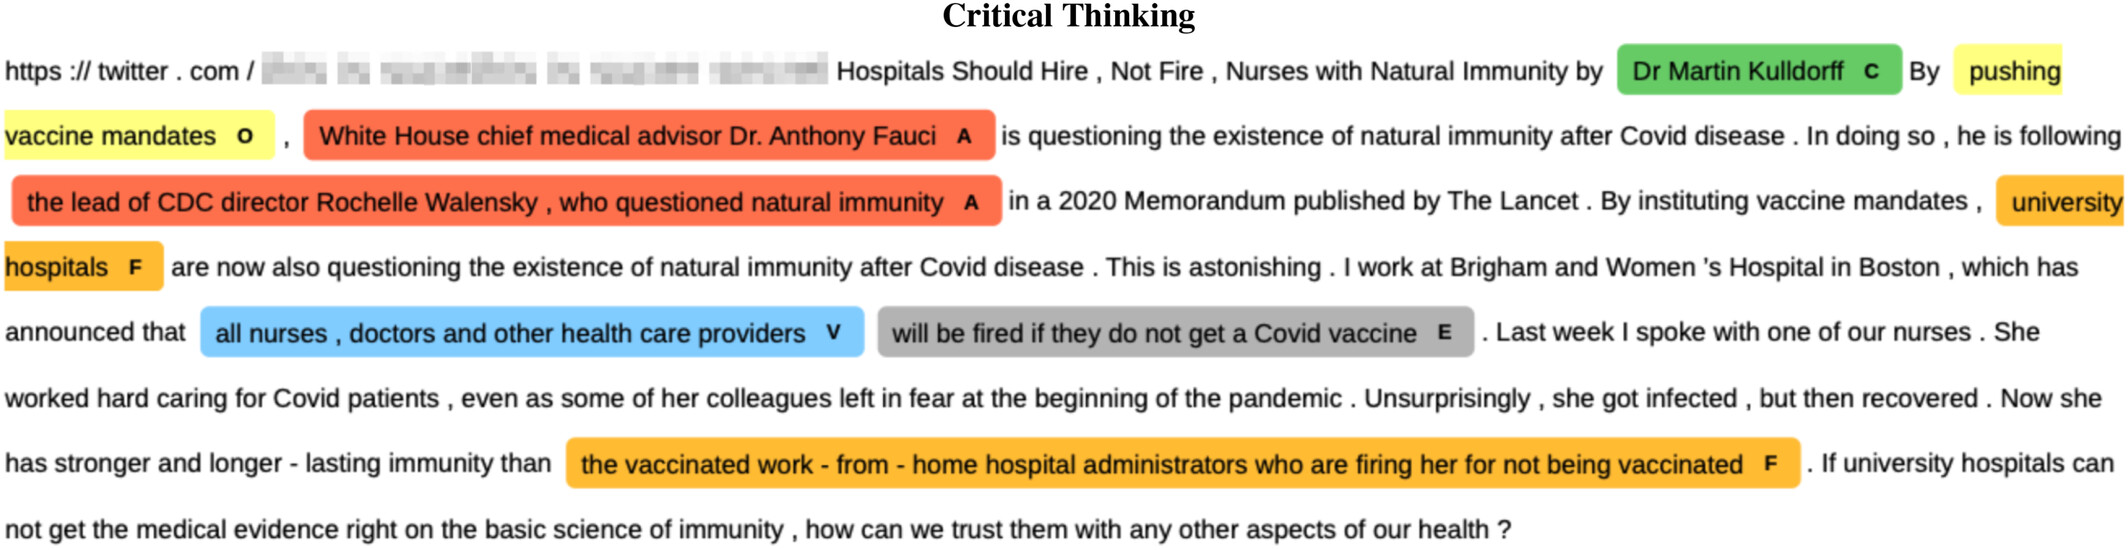
\includegraphics[width=1\textwidth]{Images/critical_thinking_annotation.png}
    }
    \vspace{0.5cm} 
    \subfloat[A conspiracy message annotated with elements of oppositional narrative \label{fig:conspiracy_theory_annotation}]{
        %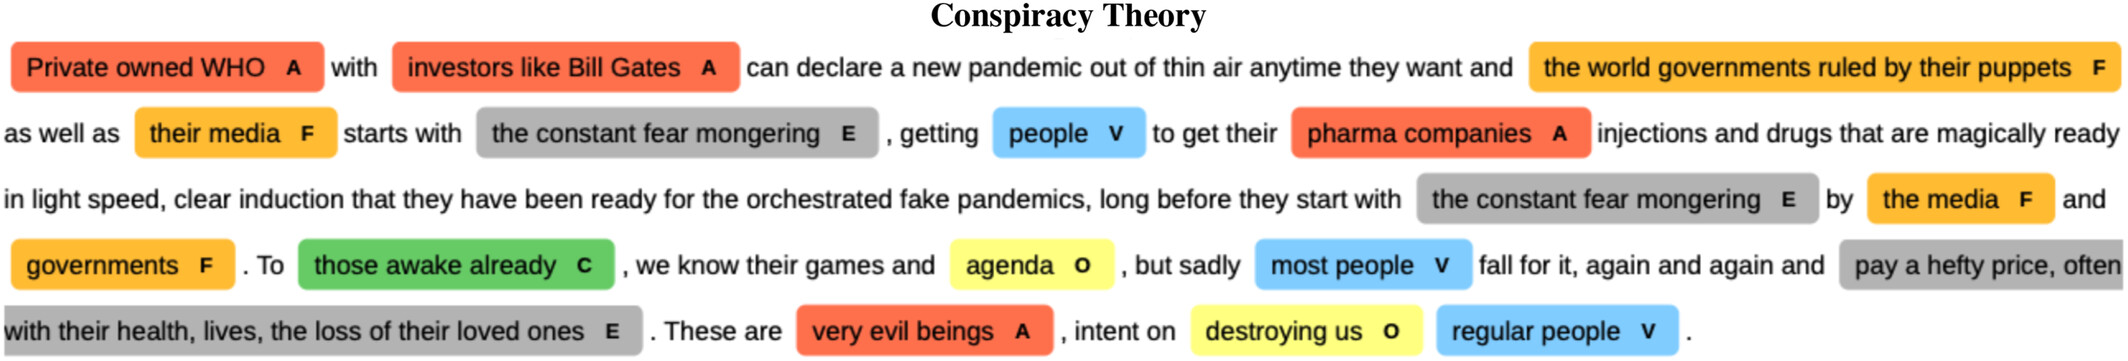
\includegraphics[width=1\textwidth, height=0.18\textheight]{conspiracy_theory_annotation}
        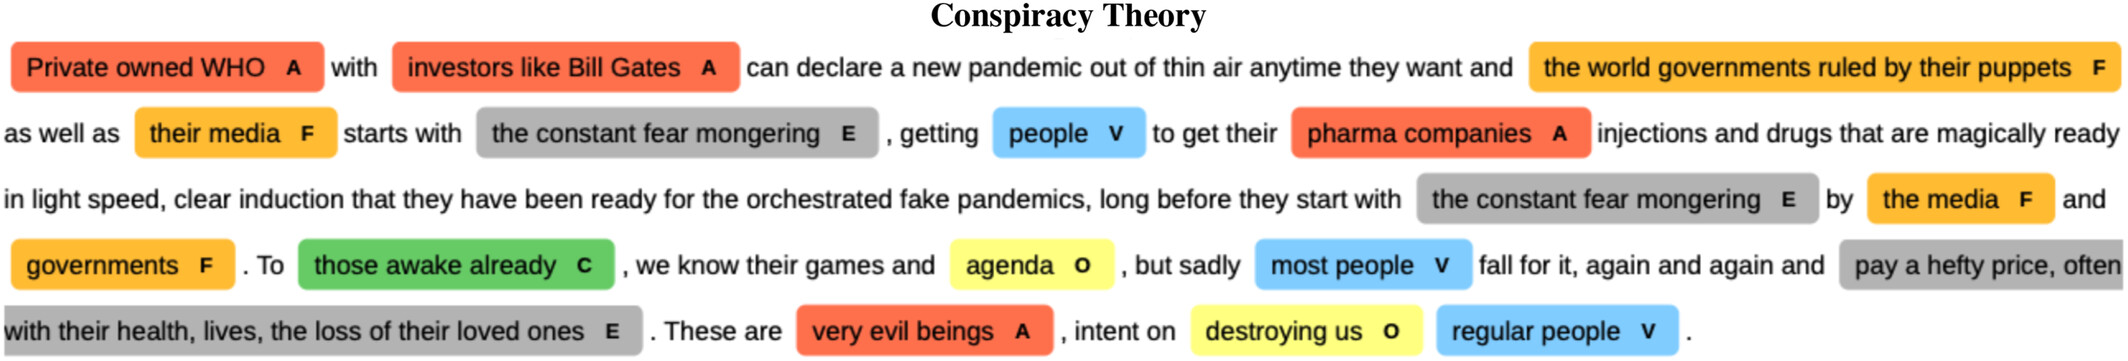
\includegraphics[width=1\textwidth]{conspiracy_theory_annotation}
    }
    \vspace{0.5cm} 
    \caption{A conspiracy and a critical message annotated with elements of oppositional narrative: Agents (A), Facilitators (F), Campaigners (C), Victims (V), Objectives (O) and Negative Effects (E) \cite{korenvcic2024distinguishes}}
    \label{fig:critical_conspiracy_annotation}
\end{figure}
\FloatBarrier

%%%%%%%%%%%%%%%%%%%%%%%%%%%%%%%%%%%%%%%%%%%%%%%%%%%%%%%%%
\subsection{Distribution of Span Categories} \label{subsec:distribution_span_categories}
As shown in Figures \ref{fig:distr_span_en} and \ref{fig:distr_span_es} and in Table \ref{tab:label_distribution_2}, the distribution of key elements within oppositional narratives varies significantly between the English and Spanish datasets, indicating potential differences in narrative focus.

\begin{figure}[h]
    \centering
    \subfloat[\small Distribution of span text categories for the English dataset \label{fig:distr_span_en}]{
        %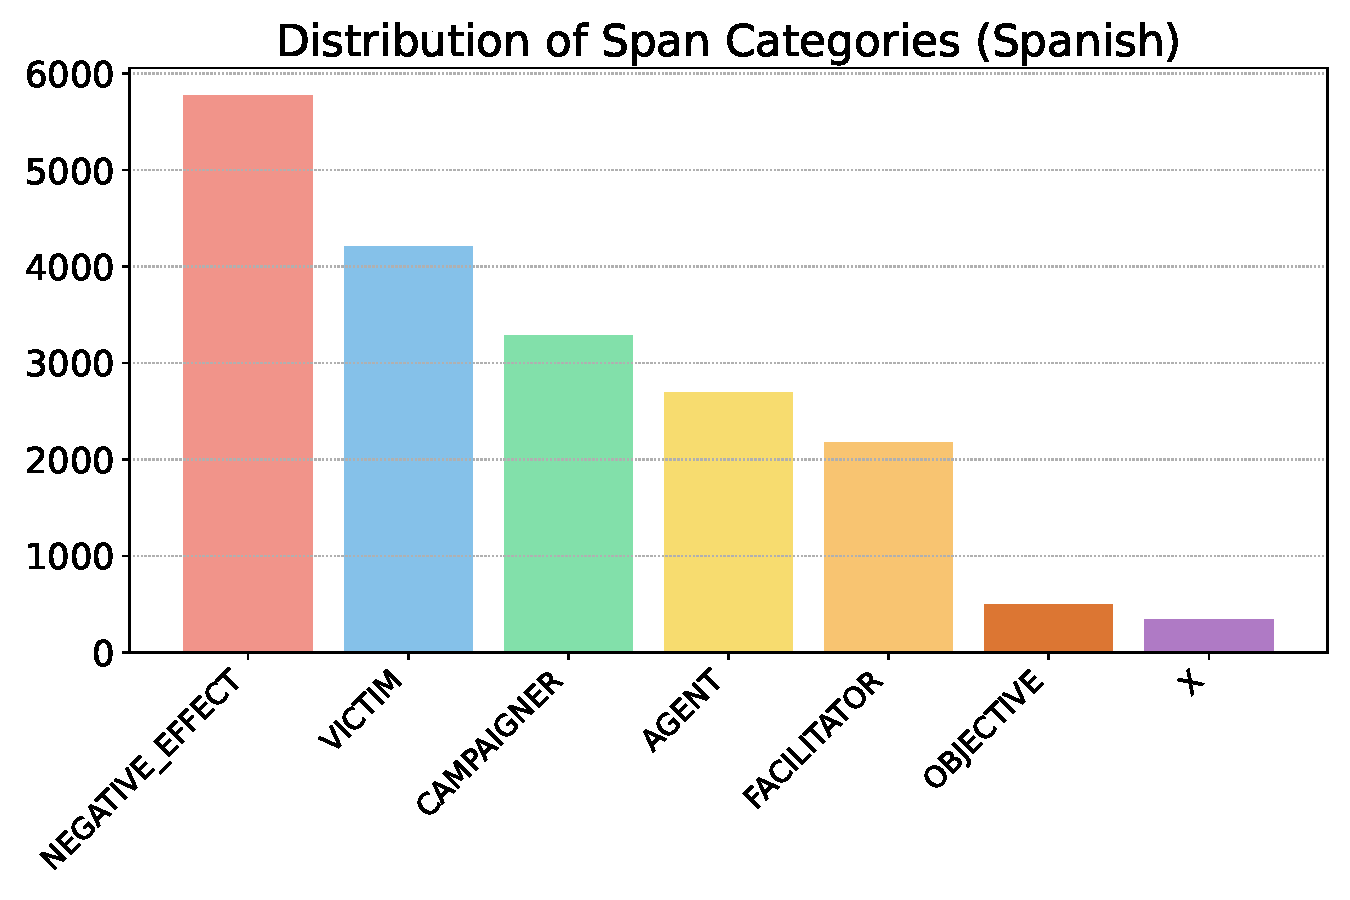
\includegraphics[width=0.9\textwidth, height=0.45\textheight]{Images/span_category_counts_t2_es_v4.pdf}
        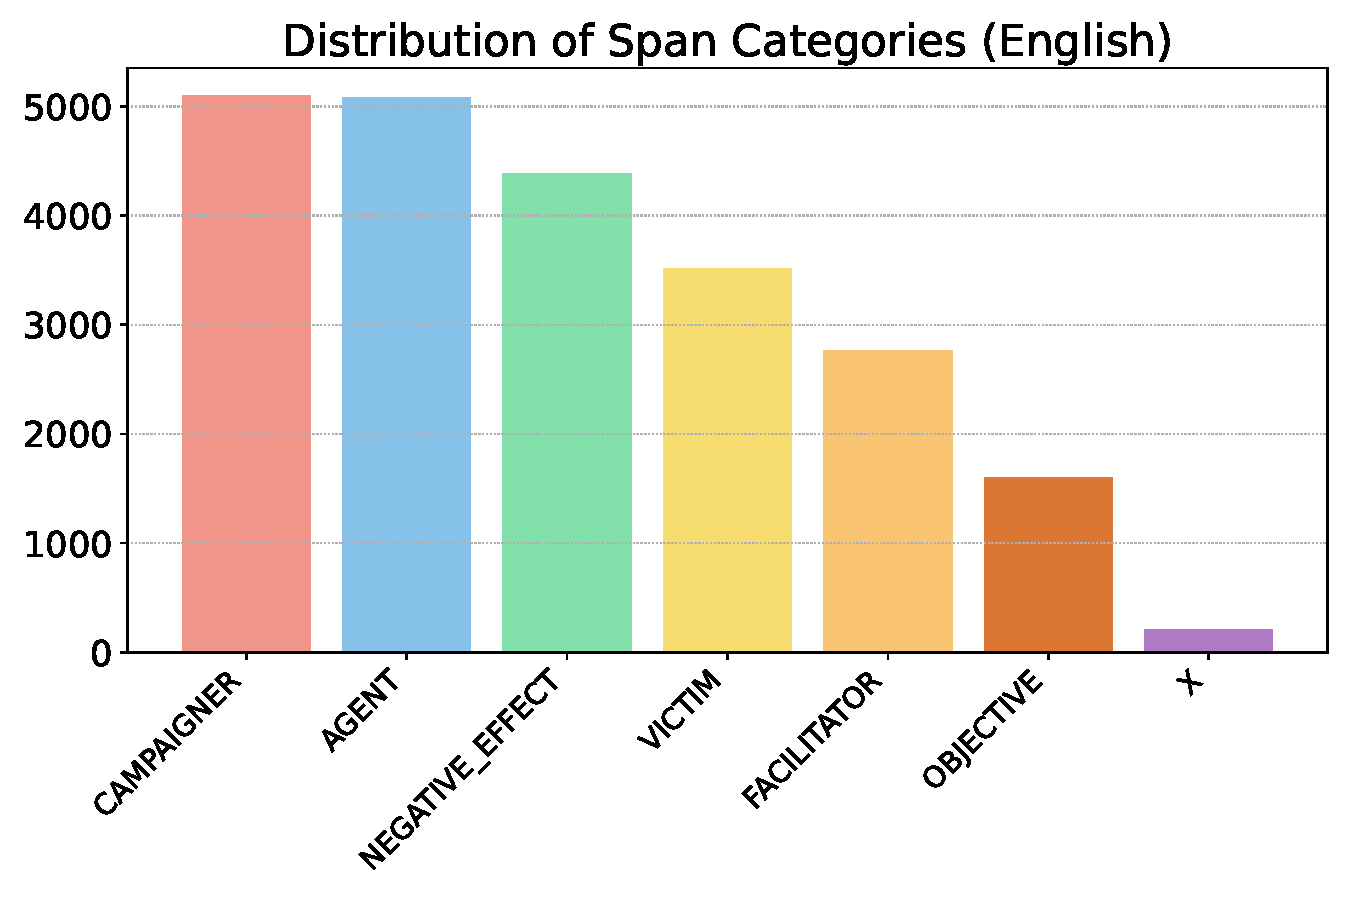
\includegraphics[width=0.90\textwidth]{Images/span_category_counts_t2_en_v4.pdf}
    }
    \vspace{0.1em} % Add vertical space between the subfigures if needed
    %\vspace{-0.5em}
    \subfloat[Distribution of span text categories for the Spanish dataset \label{fig:distr_span_es}]{
        %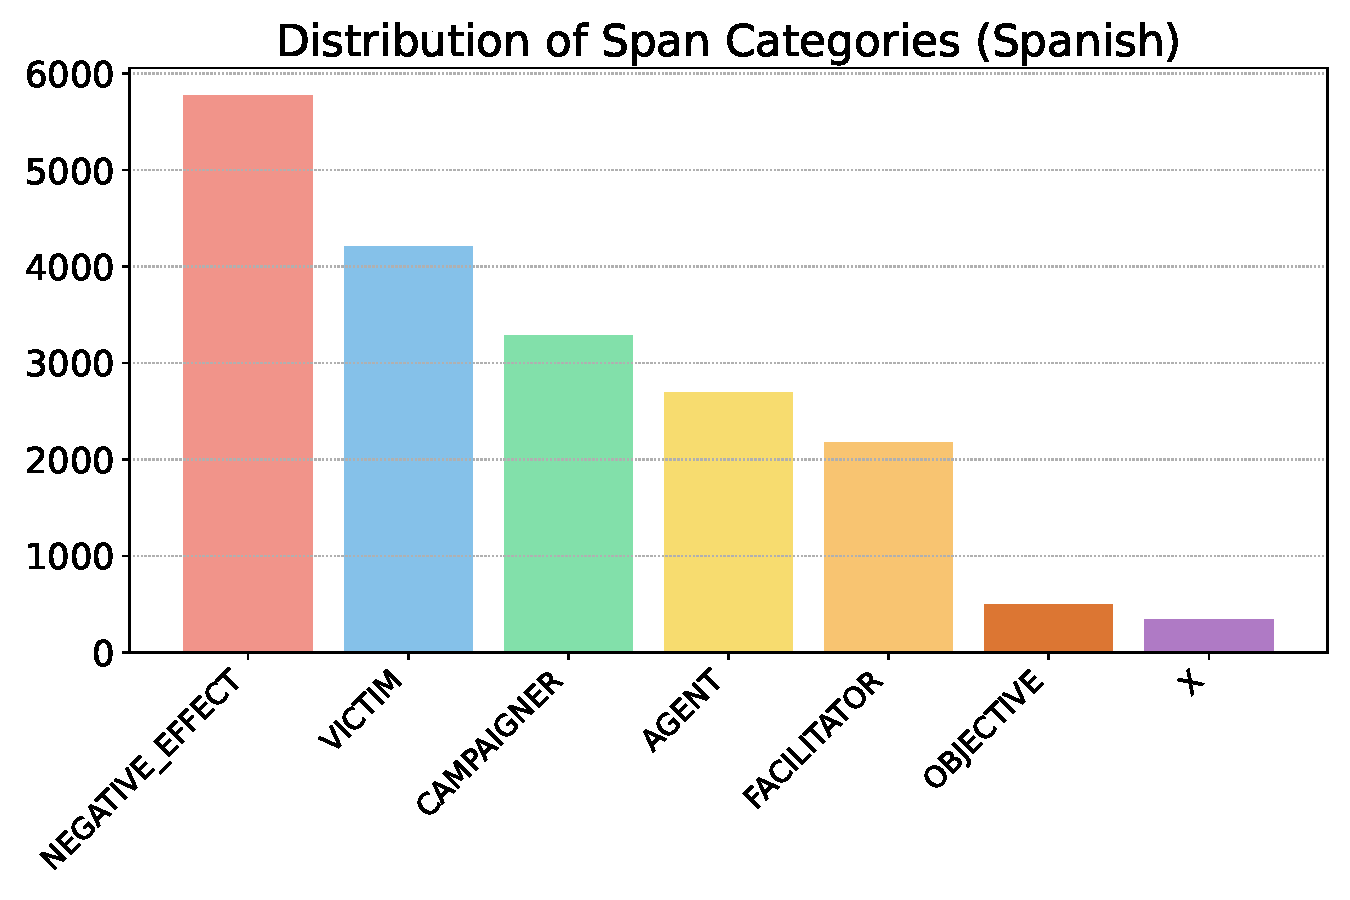
\includegraphics[width=0.9\textwidth, height=0.45\textheight]{Images/span_category_counts_t2_es_v4.pdf}
        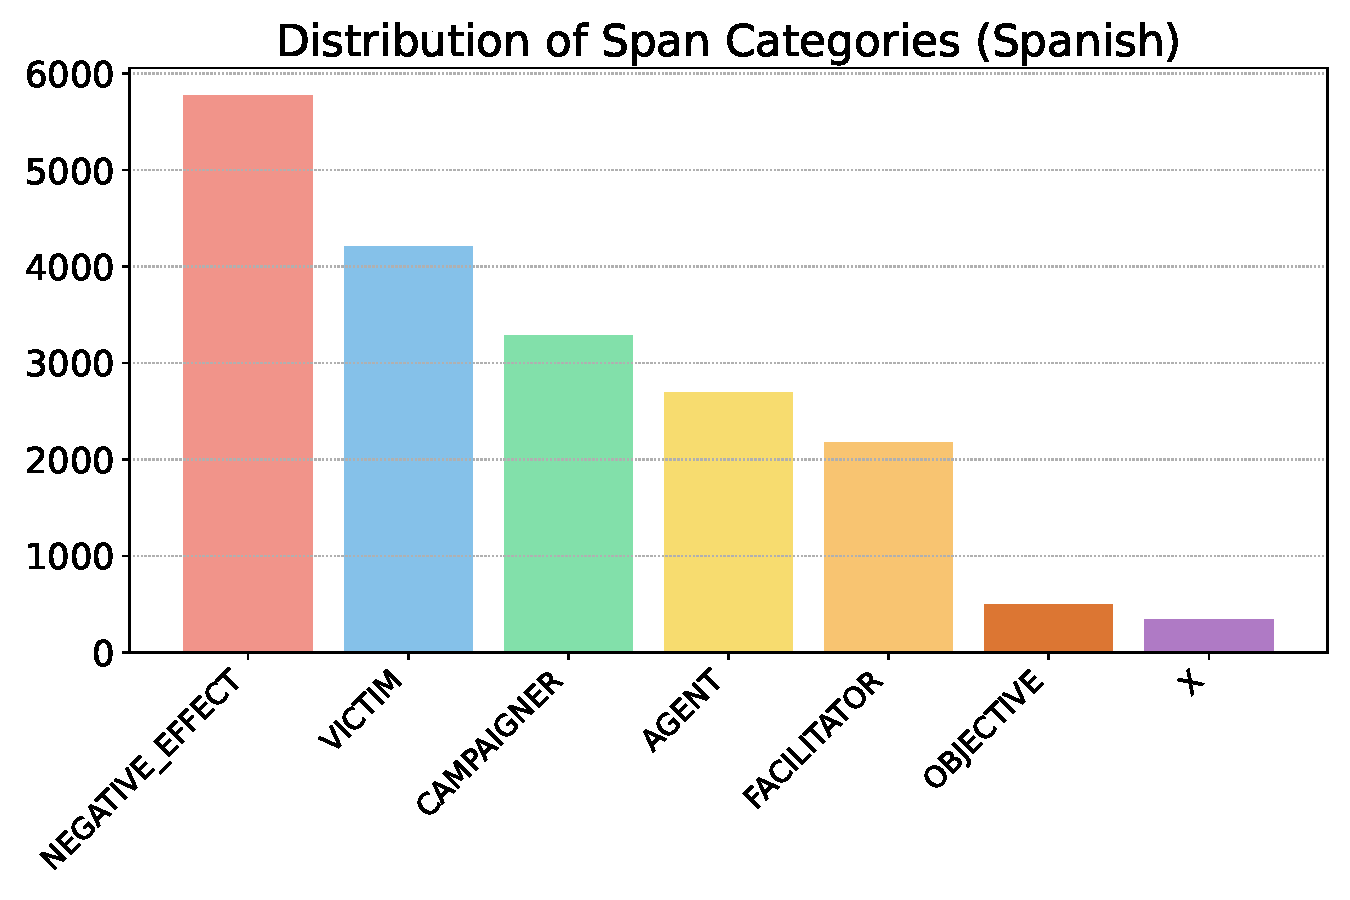
\includegraphics[width=0.90\textwidth]{Images/span_category_counts_t2_es_v4.pdf}
    }
    \caption{Distribution of span text categories for English and Spanish train datasets. The label "x" represents the texts where no label appears for the task.}
    \label{fig:span_distributions}
\end{figure}
\FloatBarrier


\begin{table}[H]
    \centering
    %\small
    %\renewcommand{\arraystretch}{0.9}
    \begin{tabular}{lcccc}
        \hline
        \textbf{Label} & \textbf{English} & \textbf{(\%)} & \textbf{Spanish} & \textbf{(\%)} \\
        \hline
        CAMPAIGNER       & 5096 & 22.70\% & 3285 & 17.63\% \\
        AGENT            & 5082 & 22.63\% & 2698 & 14.47\% \\
        NEGATIVE\_EFFECT & 4387 & 19.54\% & 5770 & 30.96\% \\
        VICTIM           & 3517 & 15.67\% & 4213 & 22.61\% \\
        FACILITATOR      & 2763 & 12.31\% & 2174 & 11.67\% \\
        OBJECTIVE        & 1602 & 7.14\%  & 493  & 2.65\% \\
        \hline
    \end{tabular}
    \caption{Distribution of span text labels for English Spanish train datasets}
    \label{tab:label_distribution_2}
\end{table}
\FloatBarrier

In the English dataset, the categories of CAMPAIGNER and AGENT are more prominently represented, with counts of 5096 and 5082, respectively. This suggests that English texts may place a stronger emphasis on identifying and challenging the actors involved in conspiracies. In contrast, the Spanish dataset has a significantly higher count of NEGATIVE\_EFFECT span texts (5770), indicating a focus on the consequences and impacts of the events described.

The notable differences in span distributions between the English and Spanish datasets underscore the importance of understanding cultural and linguistic nuances in conspiracy narratives. The English dataset's broader focus on actors and their goals might reflect different narrative styles or emphases compared to the Spanish dataset, which concentrates more on the effects and victims. These differences could stem from varying annotation guidelines or cultural perspectives on conspiracy theories.

\subsection{In-Depth Analysis of Span-Level Labels in English and Spanish on the Train Datasets}
Figure \ref{fig:grouped_chart_en} provides a visual overview of the distribution, while Table \ref{tab:distribution_categories_by_binary_labels_en} gives a detailed breakdown of these categories. The contrast between the CONSPIRACY and CRITICAL texts highlights distinctive narrative strategies and focuses. 

Examining the distribution of span-level labels in conspiracy and critical texts within the English dataset offers intriguing insights into how these narratives are framed and what elements are emphasized.

\begin{comment}
\label{subsec:in_depth_analysis_en}
\begin{figure}[h!]
 \centering
 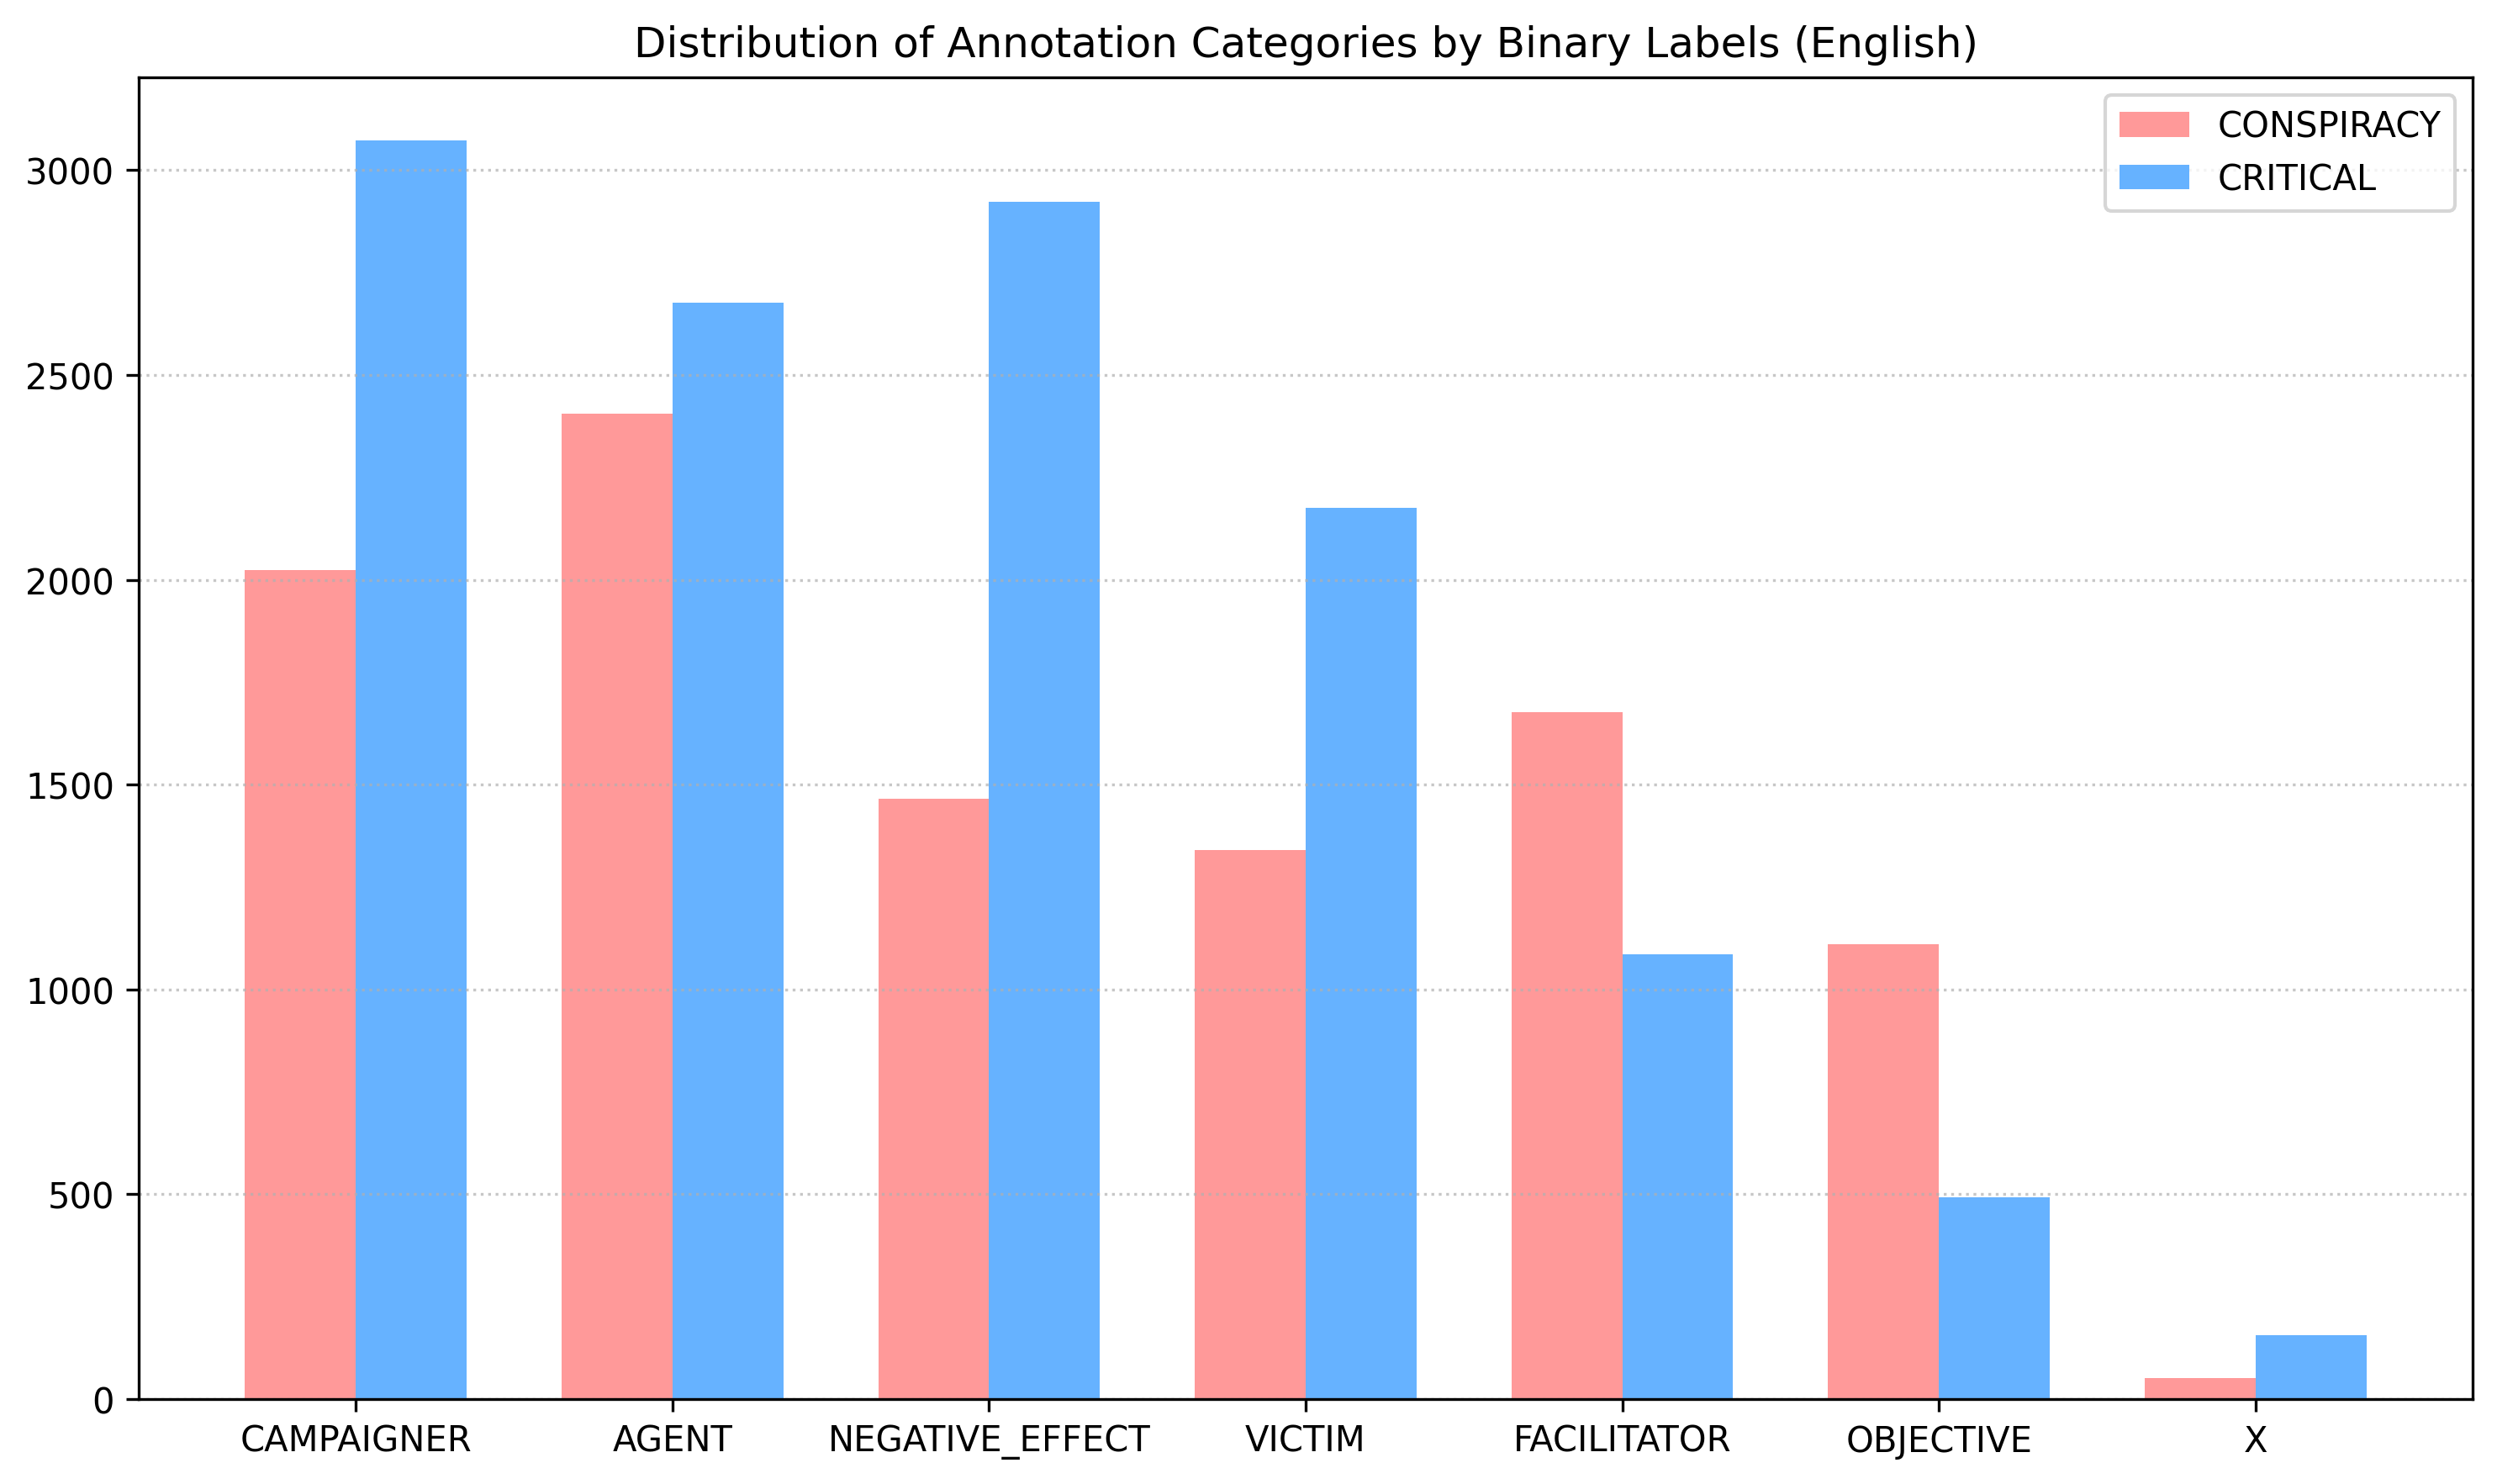
\includegraphics[width=0.86\linewidth, height=0.33\textheight]{Images/grouped_chart_en.png}
 \caption{Distribution of Categories by Binary Labels in English}
 \label{fig:grouped_chart_en}
\end{figure}
\FloatBarrier
\end{comment}

\label{subsec:in_depth_analysis_en}
\begin{figure}[H]
 \centering
 %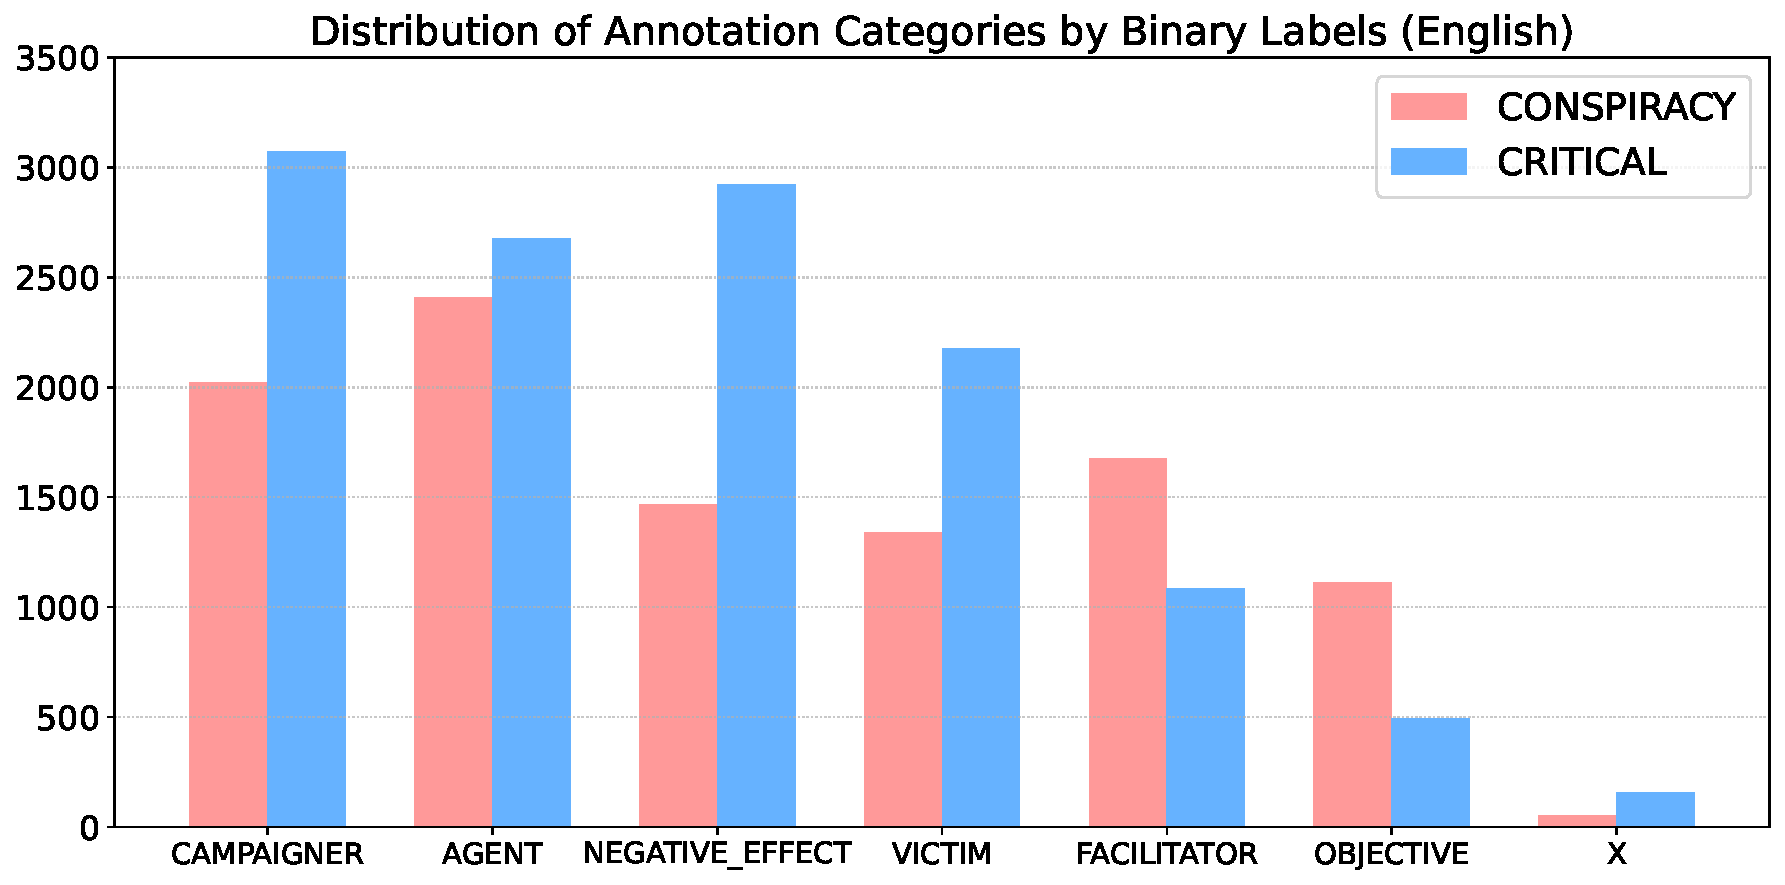
\includegraphics[width=0.86\linewidth, height=0.33\textheight]{Images/grouped_chart_en_v2.pdf}
 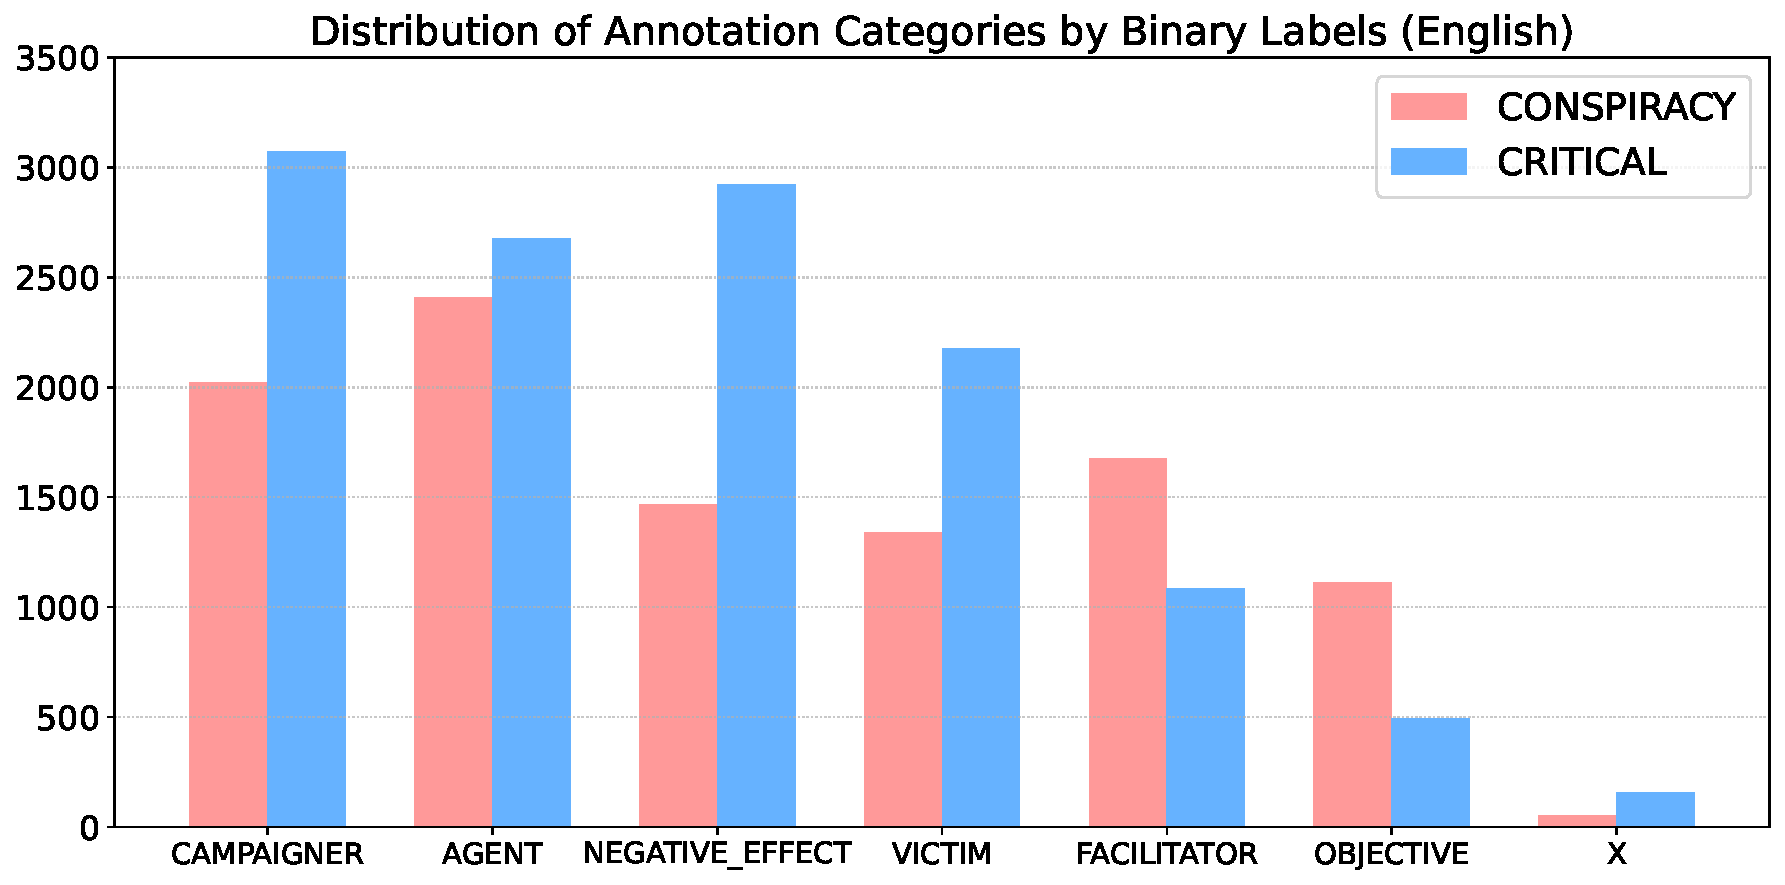
\includegraphics[width=0.95\linewidth]{Images/grouped_chart_en_v2.pdf}
 \caption{Distribution of categories by binary labels in English}
 \label{fig:grouped_chart_en}
\end{figure}
\FloatBarrier

\begin{table}[H]
 \centering
 \begin{tabular}{lcccc}
 \hline
 \textbf{Span Category}     & \textbf{CONSPIRACY} & \textbf{(\%)} & \textbf{CRITICAL} & \textbf{(\%)} \\
 \hline
 NEGATIVE\_EFFECT  & 1465      & 33.39\%     & 2922    & 66.61\%    \\
 AGENT             & 2406      & 47.34\%     & 2676    & 52.66\%  \\
 CAMPAIGNER        & 2023      & 39.68\%     & 3073    & 60.32\%  \\
 VICTIM            & 1341      & 38.13\%     & 2176    & 61.87\%  \\
 FACILITATOR       & 1677      & 60.70\%     & 1086    & 39.30\%  \\
 OBJECTIVE         & 1110      & 69.29\%     & 492     & 30.71\%  \\
 X                 & 50        & 24.27\%     & 156     & 75.73\%  \\
 \hline
 \end{tabular}
 \caption{Distribution of categories by binary labels in English}
 \label{tab:distribution_categories_by_binary_labels_en}
\end{table}
\FloatBarrier

Starting with the NEGATIVE\_EFFECT category, critical texts exhibit a significantly higher frequency of annotations, with 2922 instances (66.61\%) compared to 1465 instances (33.39\%) in conspiracy texts. This disparity suggests that critical narratives place a greater emphasis on the negative repercussions of the events being discussed, highlighting the adverse societal or individual impacts of conspiracies. The high volume of annotations in this category indicates that critical texts are particularly concerned with illustrating the harmful impacts of the events or decisions, which aligns with a narrative strategy focused on the broader consequences of these phenomena.

In contrast, the AGENT category is notably prominent in conspiracy texts, accounting for 2406 annotations (47.34\%), and remains significant in critical texts with 2676 annotations (52.66\%). This suggests that conspiracy narratives are heavily focused on identifying and scrutinizing the individuals or entities driving the conspiracies. The higher percentage in conspiracy texts underscores a narrative strategy aimed at pinpointing and examining the key players involved, reflecting a desire to assign responsibility and understand the roles of specific actors in these narratives.

The CAMPAIGNER category also exhibits an important distribution. Conspiracy texts have 2023 annotations (39.68\%), whereas critical texts have 3073 annotations (60.32\%). The higher percentage in critical texts suggests that critical narratives focus more on individuals actively challenging mainstream narratives, emphasizing the opposition to conspiratorial ideas rather than promoting them. This dynamic highlights how critical texts are more concerned with understanding and addressing the resistance to conspiracies rather than propagating them.

In contrast, the VICTIM category presents 1341 annotations (38.13\%) in conspiracy texts and 2176 annotations (61.87\%) in critical texts. The more significant representation of victims in critical texts points to an in-depth exploration of the harm caused by conspiracies, likely emphasizing the societal and personal impacts more critically than conspiracy texts, which may downplay the suffering caused by these narratives.

The FACILITATOR category is particularly striking in conspiracy texts, having 1677 annotations (60.70\%), compared to the 1086 annotations (39.30\%) in critical texts. This suggests that conspiracy narratives place considerable focus on those who enable or support the conspiratorial activities. The higher proportion in conspiracy texts highlights a narrative concern with understanding the support structures and individuals who assist in the execution of conspiracies, pointing to a more complex view of how conspiracies are carried out and sustained.

Finally, the OBJECTIVE annotations are most prevalent in conspiracy texts, with 1110 annotations (69.29\%), compared to the 492 annotations (30.71\%) contained in critical texts. This significant difference implies that conspiracy narratives are particularly concerned with the underlying goals and aims of the conspiratorial activities. The focus on OBJECTIVE reflects an interest in understanding the motivations and purposes behind the conspiracies, contrasting with critical texts that are less concerned with these aspects and more focused on immediate impacts.

These span-level label distributions indicate distinct narrative approaches in English texts. Conspiracy narratives focus heavily on agents and facilitators, aiming to dissect the individuals responsible and their intentions. This suggests a more investigative tone, as these texts delve into who is behind the conspiracies and what they aim to achieve. Critical texts, on the other hand, place a greater emphasis on the negative effects and victims, underscoring the damage caused by conspiracies. This divergence highlights two primary focuses: while conspiracy narratives are interested in unraveling the "who" and "why," critical texts are more concerned with examining the "what", the real-world consequences of these actions.

\label{subsec:in_depth_analysis_en}
\begin{figure}[H]
 \centering
 %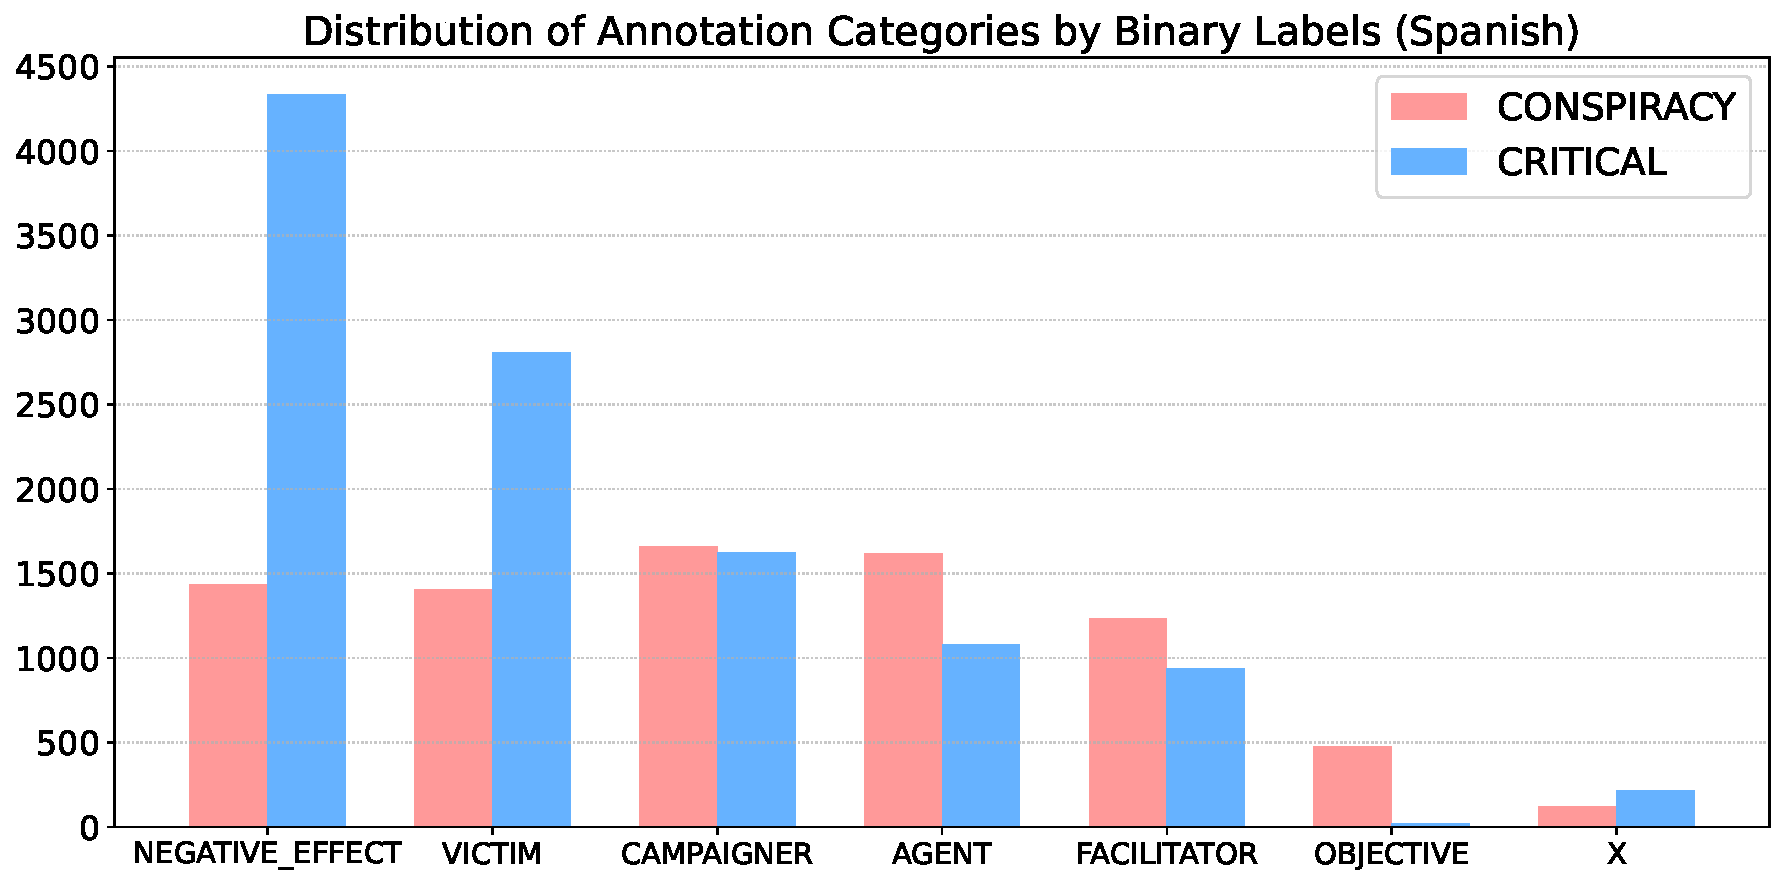
\includegraphics[width=0.86\linewidth, height=0.33\textheight]{Images/grouped_chart_es_v2.pdf}
 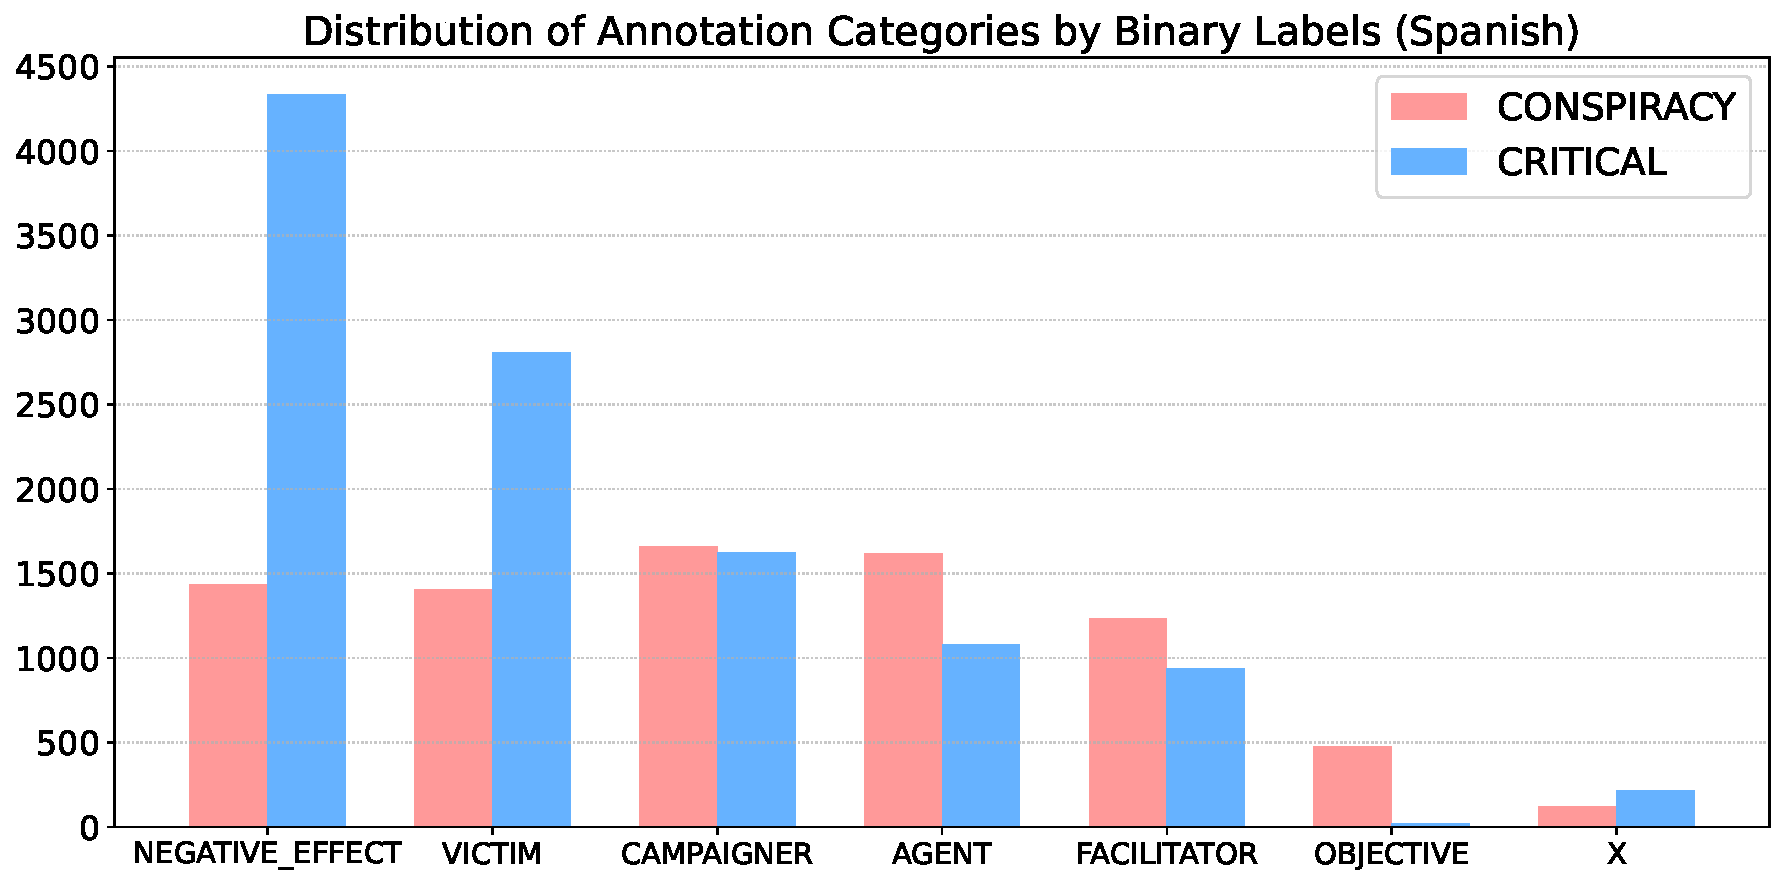
\includegraphics[width=0.95\linewidth]{Images/grouped_chart_es_v2.pdf}
  \caption{\small Distribution of categories by binary labels in Spanish}
 \label{fig:grouped_chart_es}
\end{figure}
\FloatBarrier

\begin{table}[H] 
 \centering 
 \small
 \begin{tabular}{lcccc} 
 \hline 
\textbf{Span Category} & \textbf{CONSPIRACY} & \textbf{(\%)} & \textbf{CRITICAL} & \textbf{(\%)} \\
 \hline 
 NEGATIVE\_EFFECT    & 1433 & 24.83\% & 4337 & 75.17\%   \\ 
 AGENT               & 1621 & 60.07\% & 1077 & 39.93\%   \\ 
 CAMPAIGNER          & 1662 & 50.59\% & 1623 & 49.41\%   \\
 VICTIM              & 1408 & 33.42\% & 2805 & 66.58\%   \\ 
 FACILITATOR         & 1236 & 56.87\% & 938  & 43.13\%   \\ 
 OBJECTIVE           & 475  & 96.34\% & 18   & 3.66\%    \\ 
 X                   & 123  & 36.18\% & 217  & 63.82\%   \\ 
 \hline 
 \end{tabular} 
 \caption{\small Distribution of categories by binary labels in Spanish} 
 \label{tab:distribution_categories_by_binary_labels_es} 
\end{table}
\FloatBarrier

In the case of the Spanish dataset, the span-level label distribution is illustrated in Figure \ref{fig:grouped_chart_es} and a detailed numerical breakdown is provided in Table \ref{tab:distribution_categories_by_binary_labels_es}.

In the NEGATIVE\_EFFECT category, there is a marked difference between the two types of texts. Critical texts overwhelmingly dominate this category, with 4337 annotations (75.17\%) compared to just 1433 annotations (24.83\%) in conspiracy texts. This suggests that critical texts in Spanish are more focused on illustrating the harmful consequences of the events described. This narrative approach emphasizes the severity and broader impacts of the issues, reflecting a strategy that highlights the negative repercussions for individuals and society.

On the other hand, the AGENT category shows a stronger presence in conspiracy texts, accounting for 1621 annotations (60.07\%) versus 1077 annotations (39.93\%) in critical texts. This indicates that Spanish conspiracy narratives place a significant emphasis on identifying and scrutinizing the key individuals or entities behind the conspiracies. This focus suggests a narrative strategy aimed at understanding and exposing the orchestrators of these conspiracies.

The CAMPAIGNER category is almost evenly split between conspiracy (50.59\%) and critical (49.41\%) texts, respectively of 1662 and 1623 annotations. The similar distribution suggests that both types of texts focus equally on those challenging conventional views.

When it comes to the VICTIM category, critical texts again show a notable emphasis, with 2805 annotations (66.58\%) compared to 1408 annotations (33.42\%) in conspiracy texts. This suggests that Spanish critical texts focus more on the impact and experiences of those affected by conspiracies, highlighting the personal and societal consequences in their narratives.

The FACILITATOR category is more prevalent in conspiracy texts, with 1236 annotations (56.87\%), than in critical texts, were is represented by 938 annotations (43.13\%). This suggests that conspiracy narratives have a stronger focus on those who enable or support the conspiracies, providing insight into the support structures and individuals involved in these activities.

Although the OBJECTIVE category shows a striking disparity, with conspiracy texts dominating at 475 annotations (96.34\%) compared to only 18 annotations (3.66\%) in critical texts, the overall number of OBJECTIVE span-texts is relatively low. This means that, despite the high percentage within conspiracy texts, the absolute presence of this category is not particularly significant.

Overall, the distribution of span-level labels in the Spanish dataset reveals distinct narrative patterns compared to the English dataset. Spanish conspiracy texts emphasize key players, focusing heavily on the agents' actions and their aims. Critical texts, by contrast, highlight the negative effects and victims, placing more emphasis on the outcomes of conspiratorial actions. This suggests that Spanish narratives approach conspiracies with a different lens, concentrating on the motivations and actions of the key figures in conspiracy narratives, while critical texts focus on the harm inflicted by these actions. These differences may stem from cultural or linguistic variations in how conspiracy and critical narratives are framed, providing insight into how Spanish texts conceptualize the causes and effects of conspiratorial thinking. Understanding these narrative strategies allows for a clearer view of how conspiracies and critical issues are discussed in Spanish contexts.

\subsection{Comparative Analysis Across English and Spanish Datasets} \label{subsec:comparative_analysis_en_es}
Figure \ref{fig:comparison_chart_en_es} presents a comparative analysis of span-level categories across conspiracy and critical texts in both English and Spanish datasets, merging the two figures previously seen. The dotted lines represent the Spanish dataset while the bars with solid colors represent the English dataset.

\begin{figure}[H]
 \centering
 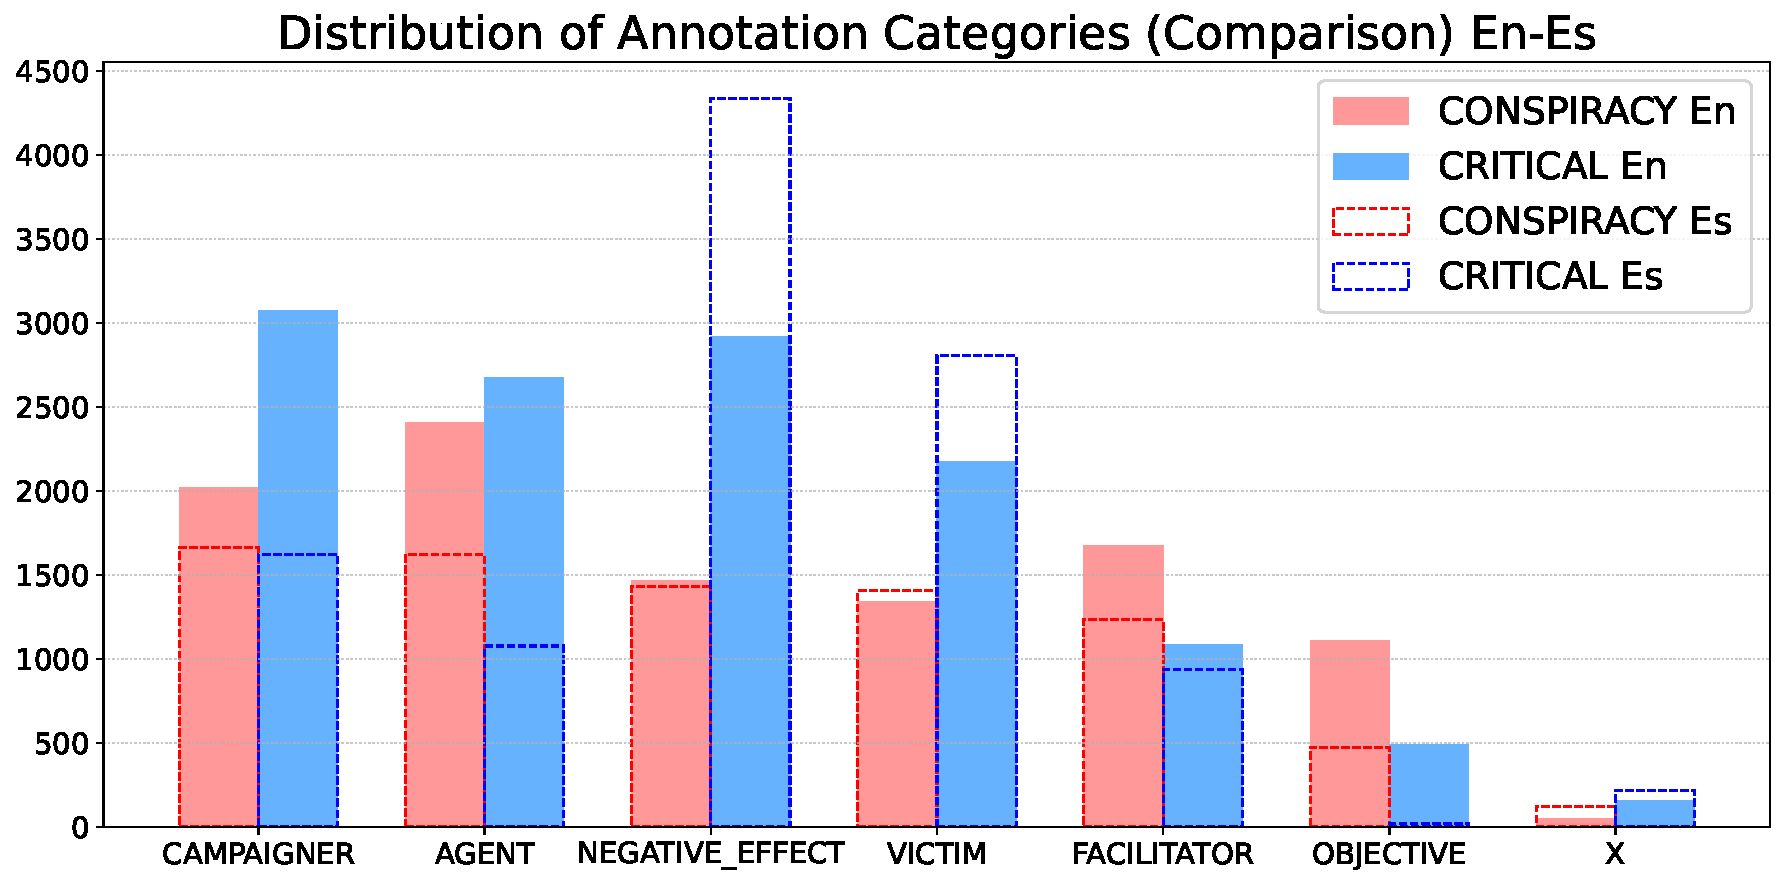
\includegraphics[width=0.95\linewidth]{Images/distrib_annotation_cat_comparison_en_es.pdf}
 \caption{\small Distribution of annotation categories: comparison}
 \label{fig:comparison_chart_en_es}
\end{figure}
\FloatBarrier

In general, the Spanish dataset shows a pronounced disparity between conspiracy and critical texts, especially in categories such as NEGATIVE\_EFFECT and VICTIM, where critical texts have significantly higher counts. This suggests a stronger emphasis on the adverse impacts of conspiracies and the experiences of those affected. 
However, the difference in NEGATIVE\_EFFECT between Spanish and English critical texts is not as stark, as English critical texts also have substantial counts in this category.

Conversely, while Spanish conspiracy texts place a strong focus on AGENTS and FACILITATORS, this emphasis is even greater in English conspiracy texts, which show higher counts for both categories. This balance in English conspiracy texts contrasts with the suggestion that Spanish texts place a deeper emphasis on these categories.

In the English dataset, CAMPAIGNER and OBJECTIVE annotations reveal distinct patterns. English critical texts have a notably higher count of campaigner annotations, indicating a strong focus on those opposing conspiracies. This emphasis is also present in Spanish texts, though the distribution between conspiracy and critical texts is more balanced. In terms of OBJECTIVES, English conspiracy texts show a stronger emphasis compared to critical texts, while in the Spanish dataset, OBJECTIVES are largely confined to conspiracy texts. %The English dataset shows a more balanced approach, particularly in its distribution of CAMPAIGNER and OBJECTIVE annotations, underscoring different narrative strategies and thematic priorities across languages.

\subsection{Comparative Insights: English vs. Spanish Text Lengths} \label{subsec:comparative_insights_en_es_text_length}
Taking a further step, firstly we compared the lengths of the texts, as detailed in Table \ref{tab:text_length}. This comparison reveals that, on average, conspiratorial texts are nearly twice as long as critical texts. Specifically, English conspiratorial texts have an average length of 742.9 characters, while English critical texts average 476 characters. Similarly, Spanish conspiratorial texts average 1112 characters, whereas Spanish critical texts average 641.2 characters. This suggests that conspiratorial texts tend to be more elaborate and possibly contain more detailed arguments or narratives compared to critical texts. Additionally, in the English dataset, each text message has an average of 5.61 span annotations, while the Spanish dataset has an average of 4.66 span elements per message.

Second, we observed the standard deviation of text lengths, which indicates the variability within each category. For English texts, the standard deviation for conspiratorial texts is 740.2, compared to 479.3 for critical texts. For Spanish texts, the standard deviation for conspiratorial texts is 945.3, compared to 577.8 for critical texts. The higher standard deviation in conspiratorial texts implies greater variability in their lengths, suggesting that some conspiratorial texts are much longer or shorter than others.

Additionally, we looked at the minimum and maximum lengths of texts in each category. The shortest English critical text has 78 characters, while the longest has 4695 characters. In contrast, the shortest English conspiratorial text has 88 characters, and the longest has 4346 characters. For Spanish texts, the shortest critical text has 99 characters, and the longest has 4761 characters, whereas the shortest conspiratorial text has 123 characters, and the longest has 4313 characters. This range of lengths further highlights the tendency for conspiratorial texts to include more content, which could be due to the complexity or thoroughness of the narratives they present.

These findings are summarized in Table \ref{tab:text_length} below, which provides a detailed statistical overview of text lengths across different categories and languages:

\begin{table}[H]
\centering
\small
\begin{tabular}{l|cccccc}
\hline
        & Dataset & Count & Mean & Std Deviation & Min & Max \\
\hline
CRITICAL & English & 2621 & 476 & 479.3 & 78 & 4695 \\
         & Spanish & 2538 & 641.2 & 577.8 & 99 & 4761 \\
\hline
CONSPIRACY & English & 1379 & 742.9 & 740.2 & 88 & 4346 \\
           & Spanish & 1462 & 1112 & 945.3 & 123 & 4313 \\
\hline
\end{tabular}
\caption{\small Statistics of text lengths (expressed in characters) by category}
\label{tab:text_length}
\end{table}
\FloatBarrier

The second analysis investigated the relationship between each span element and the span categories. This was done to explore the potential connection between critical and conspiracy narratives and their respective narrative elements.

The analysis involved counting the number of span elements in each text and calculating the point-biserial correlation coefficient \cite{brown2001point} between these counts and the category of the span. Here, the gold label is treated as a binary value: zero for critical and one for conspiracy. Table \ref{tab:pearson_coeff_corr_span_texts} displays the correlation between each annotation and the category label.

Two methods were used to count the annotations. The first method used an integer to represent the number of times each annotation appeared in the text message. The second method used a boolean to indicate whether at least one annotation of a certain type was present in the text, which was then used to calculate the Phi coefficient \cite{ekstrom2011phi}. This analysis was conducted for both datasets. Generally, the boolean values showed a stronger correlation with the gold label than the count values. A stronger correlation suggests that certain narrative elements are more prevalent in texts labeled as conspiracy. Conversely, a negative correlation indicates that an element is more common in texts labeled as critical.

\begin{table}[H]
\centering
\small
\begin{tabular}{ll|cccccc}
\hline
        &         & AGENT & FACILIT. & VICTIM & CAMPAIG. & OBJEC. & NEG. EFF    \\
\hline
English & Mult    & 0.11  & 0.17   & 0.04   & 0.07  & 0.30   & -0.013           \\
        & Bin     & 0.18  & 0.17   & -0.01  & -0.05 & \textbf{0.35}   & -0.07   \\
\hline
Spanish & Mult    & 0.18  & 0.17   & -0.04  & 0.12  & 0.32   & -0.11            \\
        & Bin     & 0.17  & 0.12   & 0.12   & -0.10 & \textbf{0.37}   & -0.23   \\
\hline
\end{tabular}
\caption{\small Pearson coefficient correlation for the appearance of annotations in a text with the gold label category}
\label{tab:pearson_coeff_corr_span_texts}
\end{table}
\FloatBarrier


In Figure \ref{fig:correlation_heatmap_bin_features_en}, we examine the correlations among the binary key element indicators in the English dataset. The observed mild correlations suggest that the pairs of \textit{Agent-Objective}, \textit{Victim-Negative Effect}, and \textit{Facilitator-Objective} frequently appear together. This pattern aligns with the nature of conspiracy narratives, where an \textit{Agent} pursues an Objective with the assistance of \textit{Facilitators}, which subsequently results in \textit{Negative Effects} for the \textit{Victims}. Additional analysis of the dataset can be found in Appendix \ref{chap:appendix_A}.

\begin{figure}[h] 
    \centering
    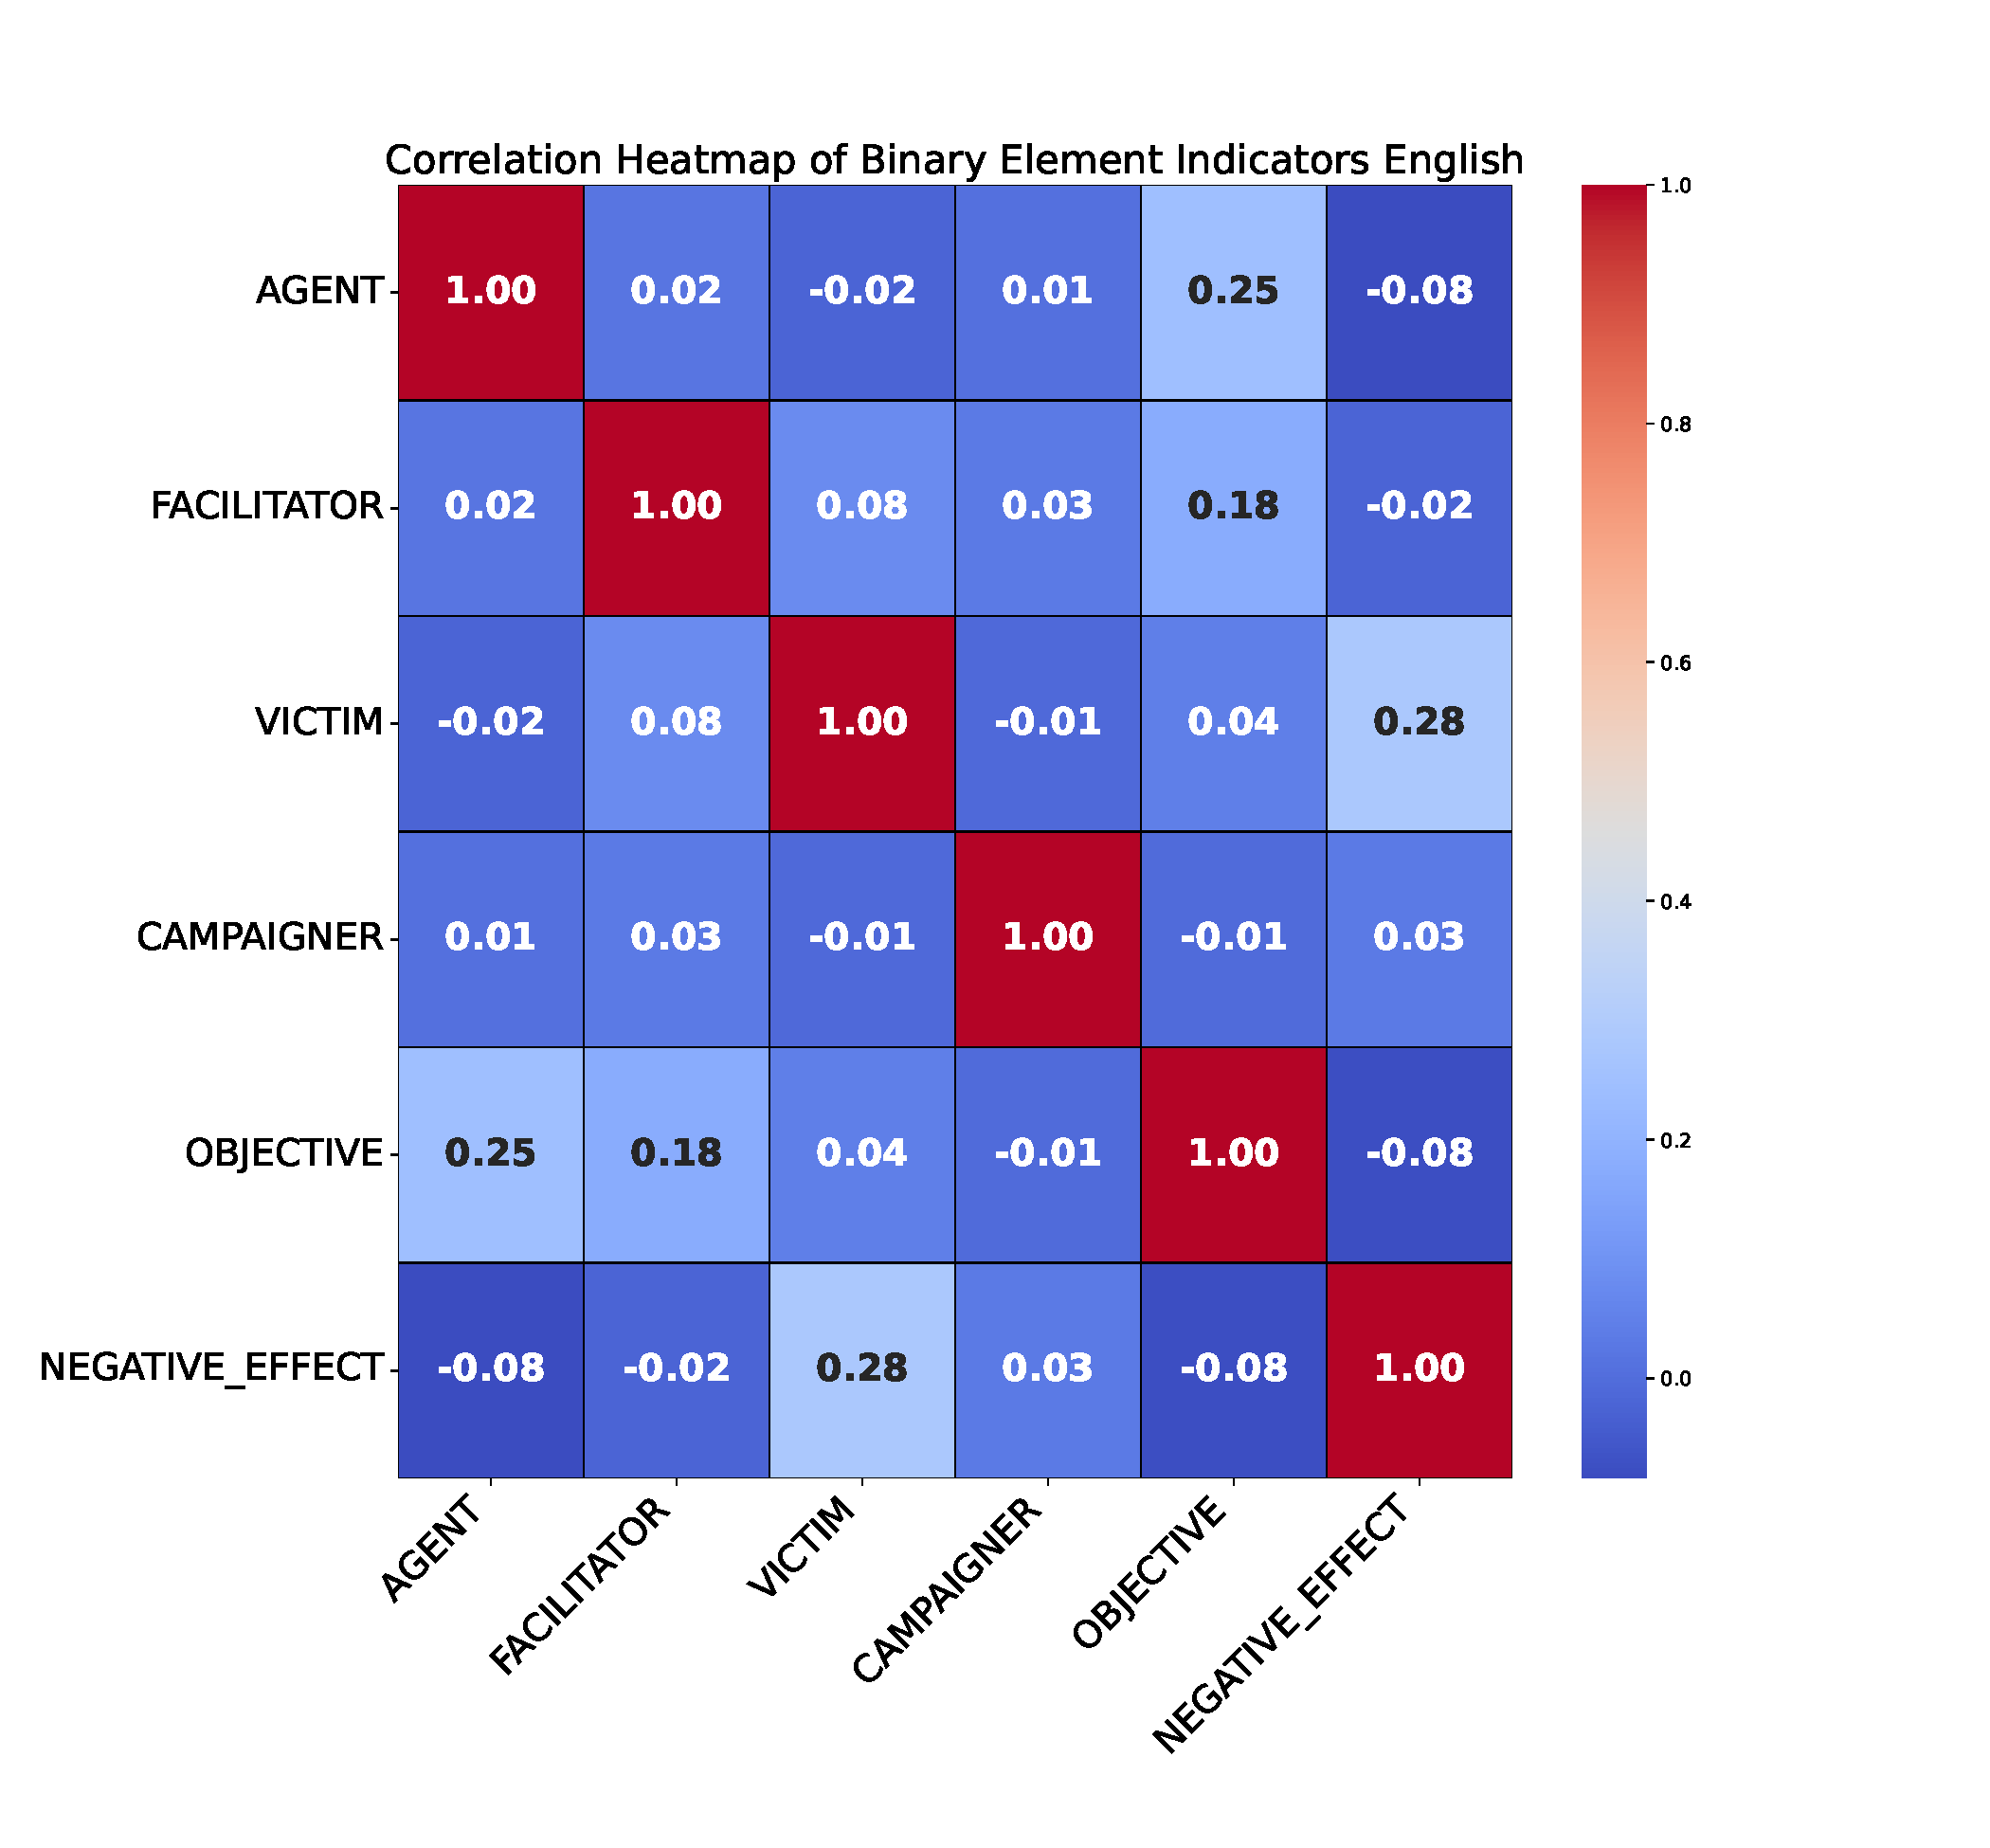
\includegraphics[width=1\textwidth]{Images/correlation_heatmap_binary_features_en_v2.pdf} 
    \caption{\small Correlation between the presence of at least one span element and other span elements in the English dataset}
    \label{fig:correlation_heatmap_bin_features_en} 
\end{figure}
\FloatBarrier

%%%%%%%%%%%%%%%%%%%%%%%%%%%%%%%%%%%%%%%%%%%%%%%%%%%%%%%%%%%%%%%%%%%%%%%%%%%%%%%%%%%%%%%%%%%%%%%%%%%%%%%
\chapter{Evaluation Metrics} \label{chap:eval_metrics}
This chapter describes the techniques employed to evaluate the models after training for both tasks. Section \ref{sec:F1_metric} provides a brief overview of the F1-score, a widely used metric in binary classification tasks. Section \ref{sec:MCC} introduces the Matthews Correlation Coefficient (MCC), highlighting its importance in evaluating binary classification models. Finally, Section \ref{sec:span_F1_metric} elaborates on Span-F1, a novel metric used for the token classification task.

\section{Accuracy and F1 Metric} \label{sec:F1_metric}
In the field of Natural Language Processing, evaluation metrics such as Accuracy and F1-score are crucial, particularly for tasks involving binary classification.

Accuracy is one of the most straightforward metrics and measures the proportion of correct predictions made by the model. It is defined as the ratio of correctly predicted instances (both true positives and true negatives) to the total number of instances:
\[
\text{Accuracy} = \frac{TP + TN}{TP + TN + FP + FN}
\]
Here, \( TP \) (True Positive) occurs when the model correctly predicts the positive class, \( TN \) (True Negative) occurs when the model correctly predicts the negative class, \( FP \) (False Positive) happens when the model incorrectly predicts the positive class, and \( FN \) (False Negative) occurs when the model incorrectly predicts the negative class.

While accuracy is intuitive and easy to compute, it can be misleading in cases where the dataset is imbalanced. For example, if 95\% of the instances belong to one class, a model that always predicts that class will achieve 95\% accuracy, despite not effectively distinguishing between classes.

The F1-score is defined as the harmonic mean of Precision (\( P \)) and Recall (\( R \)), providing a single measure that balances the trade-off between the precision and recall of a model.

Precision measures the accuracy of positive predictions made by the model. It is defined as the ratio of true positive predictions (\( TP \)) to the total positive predictions (\( TP + FP \)). Mathematically, precision is expressed as:
\[
P = \frac{TP}{TP + FP}
\]
Recall, on the other hand, measures the model's ability to identify all relevant instances within a dataset. It is defined as the ratio of true positive predictions (\( TP \)) to the total actual positive instances (\( TP + FN \)). The formula for recall is:
\[
R = \frac{TP}{TP + FN}
\]
Figure \ref{fig:true_false_pos} shows graphically \( TP \), \( FP \), \( FN \), and \( TN \) which are used for the calculations.

The F1-score is particularly important in NLP for several reasons. First, it provides a balanced evaluation metric that considers both precision and recall. This balance is essential in NLP tasks where it is critical to maintain high precision without sacrificing recall, and vice versa \cite{li2022survey}. 

Second, in many NLP applications, datasets can be imbalanced, with some classes being underrepresented. The F1-score is more informative than accuracy in such scenarios because it takes into account the model's performance on both the minority and majority classes \cite{he2009learning}. 

Third, the F1-score is the harmonic mean of precision and recall, which gives more weight to lower values. This means that the F1-score will only be high if both precision and recall are high, thus preventing a misleadingly high score in cases where one metric is significantly lower than the other \cite{powers2020evaluation}.

The F1-score is calculated as follows:
\[
F1 = 2 \times \frac{P \times R}{P + R}
\]
This formula ensures that the F1-score will be high only when both precision and recall are high. If either precision or recall is low, the F1-score will also be low, reflecting the poor performance of the model in terms of balancing false positives and false negatives.

%In NLP, evaluation metrics like Accuracy and the F1-score are widely used in tasks such as text classification, named entity recognition (NER), sentiment analysis, and more.

\begin{figure}[h]
 \centering
 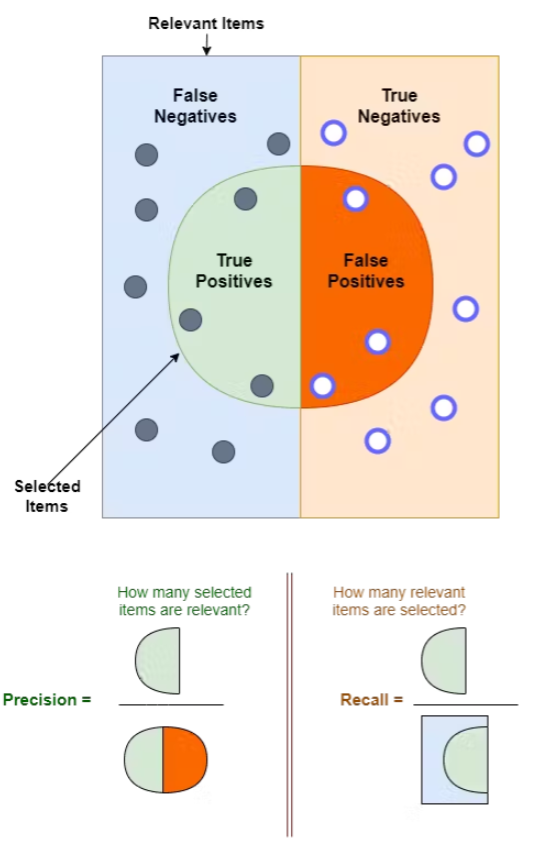
\includegraphics[width=0.53\linewidth]{TF_positive}\caption{True and false positives and negatives used for the evaluation metrics \cite{encord_metrics}}
 \label{fig:true_false_pos}
\end{figure}
\FloatBarrier

%%%%%%%%%%%%%%%%%%%%%%%%%%% FINE AGGIUNTO %%%%%%%%%%%%%%%%%%%%%%%%%%%%%%%%

\section{Matthews Correlation Coefficient} \label{sec:MCC}
The Matthews Correlation Coefficient (MCC) \cite{chicco2020advantages} is a robust metric used in binary classification tasks to evaluate the quality of predictions. It has become increasingly important in the field of Natural Language Processing due to its balanced consideration of all elements in the confusion matrix: true positives \( TP \), true negatives \( TN \), false positives \( FP \) and false negatives \( FN \). MCC is mathematically defined as:

\[
\text{MCC} = \frac{(TP \cdot TN) - (FP \cdot FN)}{\sqrt{(TP + FP)(TP + FN)(TN + FP)(TN + FN)}}
\]

This formula ensures that MCC takes into account the proportion of all four quadrants of the confusion matrix, making it a comprehensive measure. The score ranges from -1 to 1, where 1 indicates a perfect prediction, 0 suggests no better than random chance, and -1 implies total disagreement between prediction and observation.

In NLP, classification tasks such as sentiment analysis, spam detection, and named entity recognition often deal with imbalanced datasets. Traditional metrics like accuracy can be misleading because they may overestimate the performance of models on datasets with a high prevalence of one class \cite{chawla2002smote, he2009learning}.

MCC addresses this imbalance by considering all four confusion matrix components. Unlike the F1 score, which focuses primarily on precision and recall, MCC provides a more holistic evaluation by incorporating true negatives into the assessment. This comprehensive nature makes MCC particularly valuable in NLP applications where the cost of false positives and false negatives is high, and a balanced perspective on classification performance is critical \cite{chicco2020advantages, powers2020evaluation}.

One of the key advantages of MCC over metrics like accuracy, precision, recall, and even the F1 score is its ability to handle class imbalance more effectively. According to \cite{chicco2020advantages}, MCC should be preferred in binary classification tasks, especially when the dataset is imbalanced, as it provides a more rigorous and reliable measure of a model's performance. MCC's balanced approach in accounting for all aspects of the confusion matrix makes it a superior choice for evaluating classifiers.

\section{Span-F1 Metric} \label{sec:span_F1_metric}
Span-F1 is a metric used for the token classification task. It was introduced in \cite{da2020semeval} for the task on detection of propaganda techniques in news articles at the SemEval evaluation forum in 2020. Span-F1 is particularly important for tasks that involve identifying and classifying spans of text, such as the second task of the PAN challenge on detecting elements of oppositional narratives.

The metric is calculated as follows:
Assume \(d\) is a text message from a dataset \(D\). Gold spans are contiguous subsequences, \(t\), in a text message: \(t \subseteq d\). Each gold span fragment is indicated by a starting and ending integer, corresponding to its location in the text. For example, assuming a text message "Jack Robert Johnson orchestrated a secret plan to manipulate the global stock market.", the corresponding gold span element (in characters) for the Agent ("Jack Robert Johnson") label would be \(t = [0, 19]\). Let \(T_d = \{t_1, \ldots, t_n\}\) represent all the predefined gold labels \(t\) in a text message \(d\) while \(T = \{T_d\}_{d \in D}\) are the gold labels in the dataset \(D\). Similarly, let \(S_d = \{s_1, \ldots, s_n\}\) be all the predicted gold labels in \(d\), and \(S\) the same for \(D\). Building on the formulas from \cite{potthast-etal-2010-evaluation},  \cite{da2020semeval} define precision (\(P\)) and recall (\(R\)) as follows:

\[
P(S, T) = \frac{1}{|S|} \cdot \sum_{d \in D} \sum_{s \in S_d, t \in T_d} \frac{|s \cap t|}{|t|}
\]

\[
R(S, T) = \frac{1}{|T|} \cdot \sum_{d \in D} \sum_{s \in S_d, t \in T_d} \frac{|s \cap t|}{|t|}
\]

Additionally, the authors define the equations to be equal to zero for \(|S| = 0\) and \(|T| = 0\) respectively. During prediction, models may generate overlapping predictions for gold span labels. For example, a model may predict that "Jack" (\(t = [0, 4]\)) is an Agent gold label and also that "Robert Johnson" (\(t = [5, 19]\)) is as well. Another example could be predicting "Johnson" (\(t = [12, 19]\)) and "Jack Robert Johnson" (\(t = [0, 19]\)) as Agents. Since both scenarios are examples of correct predictions, the authors combine adjacent and overlapping solutions before calculating the score. Finally, the F1 score is defined as the harmonic mean between the recall and precision:

\[
F1(S, T) = 2 \cdot \frac{P(S, T) \cdot R(S, T)}{P(S, T) + R(S, T)}
\]

Span-F1 is crucial for evaluating the performance of models in tasks that require precise identification of text spans. It ensures that both precision and recall are balanced, providing a comprehensive measure of a model's ability to accurately and completely identify relevant spans within the text. This is particularly important in applications such as named entity recognition, where both false positives and false negatives can significantly impact the usefulness of the extracted information \cite{yadav2018survey}.

%%%%%%%%%%%%%%%%%%%%%%%%%%%%%%%%%%%%%%%%%%%%%%%%%%%%

\chapter{Experimental Framework} \label{chap:system_overview}
In this chapter, we outline the experimental framework developed to train, evaluate, and optimize our models across the two tasks. Section \ref{sec:strat_k_cross} begins with a discussion on the rationale behind using cross-validation, specifically explaining the use of Stratified k-fold cross validation to maintain balanced class distributions within each fold. We then delve into the experimental setup in Section \ref{sec:experiments_setup}, highlighting the methodological choices made to ensure consistency, reliability, and computational efficiency throughout our process. Subsequently, Section \ref{sec:note_on_hyperparameter_opt} will give some insights about hyperparameter optimization.

\section{Stratified K-Fold Cross Validation} \label{sec:strat_k_cross}
In machine learning tasks, it is common practice to use two different datasets for model development: a training set and a test set. The training set is used to train the model, allowing it to learn patterns from the data, while the test set is held out and used solely for evaluation. This separation ensures that the model's performance is not only optimized for the given data but also generalizes well to new, unseen data, thus preventing overfitting and providing a more accurate measure of its effectiveness.

In the context of the PAN shared task, only the training dataset was available for the majority of the work done in this thesis. Consequently, we had to rely on the training set to evaluate our model. One effective way to create such a dataset is through cross-validation. Specifically, we employed stratified k-fold cross validation, a robust method that offers several advantages for model evaluation and training.

Stratified k-fold cross validation involves partitioning the training set into $k$ subsets, or "folds", of approximately equal size, while maintaining the ratio of class labels within each fold. This stratification ensures that each fold is representative of the overall distribution of the data, which is particularly important in imbalanced datasets where some classes may be underrepresented. During each epoch of training, the model is trained $k$ times, where $k-1$ folds are used for training and the remaining fold is used for validation. The model's performance is then assessed by averaging the results across all $k$ folds and epochs, providing a comprehensive evaluation metric.

% start new part -------------------------------------------------
An essential part of this cross-validation process is the use of model checkpoints, where the best-performing model in each fold (based on validation metrics) is saved. This approach allows for careful monitoring of the model's performance during training and ensures that the best version of the model within each fold is preserved for final evaluation. By saving checkpoints, we could retrieve models trained under optimal conditions, thus avoiding potential overfitting from training on all folds without validation.

After training on each fold, an alternative way to calculate the final performance metric for the model is obtained by averaging the results from all the best checkpoints across the $k$ folds. This averaged score offers a reliable and stable measure of model performance, reflecting the model’s generalizability across different subsets of the training data.
%end new part -----------------------------------------------------

The implementation of stratified k-fold cross validation used in this thesis was facilitated by the Scikit-learn library \cite{pedregosa2011scikit}. For both binary and token classifiers, we used three folds ($k=3$). This choice strikes a balance between computational efficiency and the robustness of the validation process.

Cross-validation was crucial for obtaining reliable performance scores for our models in the absence of the official test dataset.

\begin{figure}[h]
 \centering
 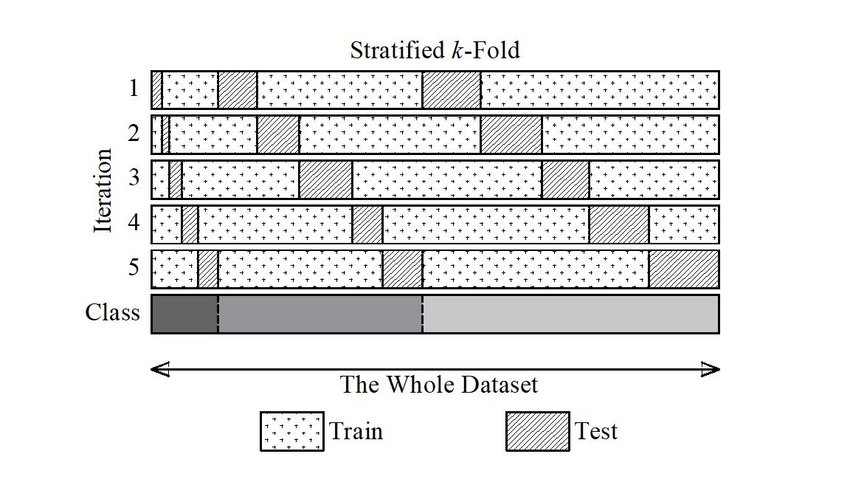
\includegraphics[width=0.87\linewidth, height=0.36\textheight]{./Images/strat_cross_val}
 \caption{Stratified k-fold cross validation. Example with k=5 \cite{stratified_cross_val}}
 \label{fig:Strat_K_fold_cross_val}
\end{figure}
\FloatBarrier


\section{Experiments Setup} \label{sec:experiments_setup}
Experiments were conducted on three NVIDIA GeForce GTX 1080 (8 GB memory). To ensure uniformity and comparability of results, 
the same experimental setting was consistently applied across all tasks, runs, and languages under study. Our experimental setup, designed for optimal performance and efficient resource utilization, utilized stratified k-fold cross validation with 3 folds, as detailed in Section \ref{sec:strat_k_cross}, to ensure robust performance across different subsets of the data. 

The training process spanned 15 epochs.A weight decay of 0.01 was applied as a regularization technique to penalize large weights.A custom linear learning rate scheduler was employed, adjusting the learning rate from an initial value of 2e-5 to a final value of 2e-6 over the total number of training epochs. 
Gradient accumulation steps were set to 4, effectively increasing the batch size without inflating the memory footprint by accumulating gradients over multiple steps before updating the model's weights. 
The training batch size per device was dynamically set based on available GPU memory, managed by a custom callback designed to dynamically adjust the batch size used during training and evaluation based on the available GPU memory.
This ensures efficient resource utilization and prevents memory-related issues during training, especially when dealing with varying data sizes and model complexities. This adaptive approach ensured optimal resource utilization without encountering memory constraints, thereby maintaining high computational efficiency and preventing potential memory-related issues during training. Upon completion of training, the best model, as determined by the F1 score, was loaded. 


In the following table we can better observe the experiment setting:
\begin{table}[H] % Use [H] to force the table to be placed here
 \centering
 \begin{tabular}{lll}
 learning rate                 & linear\_learning\_rate\_scheduler    &  \\
 evaluation\_strategy          & epoch                                &  \\
 save\_strategy                & epoch                                &  \\
 num\_train\_epochs            & 15                                   &  \\
 weight\_decay                 & 0.01                                 &  \\
 load\_best\_model\_at\_end    & True                                 &  \\
 metric\_for\_best\_model      & f1                                   &  \\
 gradient\_accumulation\_steps & 4                                    & \\
 per\_device\_train\_batch\_size   & batch\_size                      & \\
 per\_device\_eval\_batch\_size    & batch\_size                      &
 \end{tabular}
 \caption{Experiments setup for all the tasks}
 \label{tab:label_distribution}
\end{table}
\FloatBarrier 

\section{Hyperparameter Optimization} \label{sec:note_on_hyperparameter_opt}
To enhance the performance of our binary classification models, we integrated two prominent hyperparameter optimization techniques: Grid Search and Bayesian Optimization \cite{alibrahim2021hyperparameter}. Initial experiments were conducted using more compact transformer architectures, such as distilbert-base-cased\footnote{\url{https://huggingface.co/distilbert/distilbert-base-cased}} for English and 
bert-base-spanish-wwm-uncased\footnote{\url{https://huggingface.co/dccuchile/bert-base-spanish-wwm-uncased}} \cite{CaneteCFP2020} for Spanish, to assess the effects of these optimization approaches. However, the outcome did not meet expectations. The increase in F1-score was minimal (around 0.1\%), while the training duration grew significantly. This finding is consistent with existing studies, which often report that hyperparameter tuning for transformers rarely produces substantial gains for datasets containing only a few thousand samples.

The prevailing consensus in the community acknowledges that default hyperparameter configurations for models like BERT generally provide satisfactory performance for many applications. The computational cost and training time associated with exhaustive hyperparameter optimization are typically disproportionate to the incremental improvements achieved. Our results reinforced this understanding, highlighting the considerable resource demands without a corresponding payoff in performance metrics \cite{alibrahim2021hyperparameter}.

Consequently, based on our observations and a practical cost-benefit analysis, we decided against extensive hyperparameter tuning in further experiments. Instead, we prioritized exploring more impactful strategies that could yield significant improvements without imposing heavy computational burdens.

%%%%%%%%%%%%%%%%%%%%%%%%%%%%%%%%%%%%%%%%%%%%%%%%%%%%%%%%%%%%%%%%%%%%%%%%%%%%%%%%%

\chapter{Binary Classification of Conspiratorial vs. Critical Thinking} \label{chap:text_classification_task}
In this chapter, we will provide a detailed account of the experiments conducted for the binary classification task, beginning with the data augmentation techniques applied to the dataset. This will be followed by a comprehensive analysis of the experiments carried out on the train dataset, culminating in a discussion of two systems submitted for the competition.

\section{Data Augmentation} \label{sec:data_augmentation_T1}
Data augmentation was crucial in enhancing the effectiveness of the binary classification models, especially when facing with challenge like imbalanced datasets, as in our case. In such scenarios, where one class often dominates, models are prone to overfitting and biased predictions. 
Data augmentation techniques like back-translation, summarization, or paraphrasing were employed to generate varied text while preserving the original meaning. Artificially expanding the dataset enhance the model's exposure to different linguistic structures and expressions, allowing it to better capture subtle patterns in both classes, particularly the minority class. By enriching the dataset in this way, data augmentation not only improves classification performance but also helps create more resilient models that can handle real-world linguistic variability, leading to more accurate and reliable predictions.

\subsection{Summarization} \label{subsec:summarization_T1}
A first experiment involved summarizing the datasets using different models, such as T5-small\footnote{\url{https://huggingface.co/google-t5/t5-small}}, T5-base\footnote{\url{https://huggingface.co/google-t5/t5-base}}, and T5-large\footnote{\url{https://huggingface.co/google-t5/t5-large}} \cite{ni2022sentence}. Summarizing with T5-small yielded sub-optimal results due to its limited capacity, which restricted its ability to capture and compress the full context of longer or more complex texts. It struggled to balance abstraction and comprehension, resulting in outputs that merely repeated or extracted a subpart of the original text without effectively rephrasing or condensing it. The model lacked the depth to perform true abstractive summarization, where new, shortened representations are created while maintaining the full text's meaning and key details, leading to less informative and often incomplete summaries. While T5-base showed some improvement, generating slightly more balanced summaries, and T5-large performed even better with more comprehensive and coherent outputs, the results were still unsatisfactory. They fell short of ideal performance, particularly with complex, nuanced texts, where the generated summaries still missed key details or lacked the refinement expected in human-level summarization. A recurring issue across all these models, especially T5-small, was the frequent lack of coherence, producing sentences that were awkward or nonsensical. Despite the larger models having more parameters to work with, they also struggled to maintain the logical flow of information, resulting in summaries that missed key details and sometimes made little sense, ultimately failing to meet expectations for high-quality summarization.

\subsection{Paraphrasing} \label{subsec:paraphrasing_T1}
Since summarization yielded poor results, we turned to paraphrasing using the fine-tuned T5-large model. The T5 model automatically handles all the steps, including text cleaning and back-translation techniques. It processes the input text by removing unwanted characters and spaces, then introduces variations through its built-in back-translation mechanisms. The model translates the text to a secondary language (internally managed) and back, ensuring the paraphrased output remains close to the original meaning while diversifying sentence structures.

However, the results were not good enough to incorporate the newly paraphrased dataset into further experiments. The paraphrased text frequently suffered from disrupted word order, leading to nonsensical or grammatically incorrect sentences. Rather than producing meaningful variations, the model often misplaced key words or phrases, which interfered with the logical flow of the sentences and made them difficult to interpret. This issue likely stemmed from problems in the tokenization and decoding process of the T5 model, where sentences were split into subword tokens that the model struggled to recombine coherently, resulting in broken sentence structures.

Moreover, the built-in back-translation process may have introduced subtle shifts in sentence construction that further confused the paraphrasing model. These shifts, while introducing variation, also altered the original sentence structure in ways that made it harder for the model to reconstruct a coherent paraphrase.

\subsection{One-Way Translation} \label{subsec:translation_T1}
After the initial data augmentation techniques yielded unsatisfactory results, we turned to one-way translation as the final approach, taking advantage of the fact that we had two distinct datasets, one in English and one in Spanish. This process involved translating each dataset into the other language, effectively doubling the amount of data available for training. In the first trial, we employed the \textit{googletrans} Python library\footnote{\url{https://pypi.org/project/googletrans/}}, which serves as an API wrapper for Google Translate. While this approach produced satisfactory results, further testing with the Helsinki-NLP models yielded even better performance.

For the translations, we used the MarianMT\footnote{\url{https://huggingface.co/docs/transformers/model_doc/marian}} model to automate the process. The \textit{Helsinki-NLP/opus-mt-es-en}\footnote{\url{https://huggingface.co/Helsinki-NLP/opus-mt-es-en}} model was employed to translate the Spanish dataset into English, while the \textit{Helsinki-NLP/opus-mt-en-es}\footnote{\url{https://huggingface.co/Helsinki-NLP/opus-mt-en-es}} model was used for translating the English dataset into Spanish \cite{tiedemann2020opus}. The translation process began by loading the datasets, and for each entry, both the main text and any associated annotations were translated. The MarianMT model tokenized the input text, generated the translation, and decoded the output into the target language.

Translating the datasets allowed the creation of two expanded versions of the original datasets, thus effectively doubling the size of the training data. This augmentation technique significantly enriched the dataset by introducing more linguistic diversity and a wider range of sentence structures. By exposing the models to both the original and translated versions of each dataset, the models were able to learn from a greater variety of linguistic patterns, improving their ability to generalize to unseen data. Figures \ref{fig:trad_es_en} and \ref{fig:trad_en_es} provide examples of entries translated from Spanish to English and from English to Spanish, respectively, demonstrating how the core meaning of the text was preserved.

\begin{figure}[h!]
 \centering
 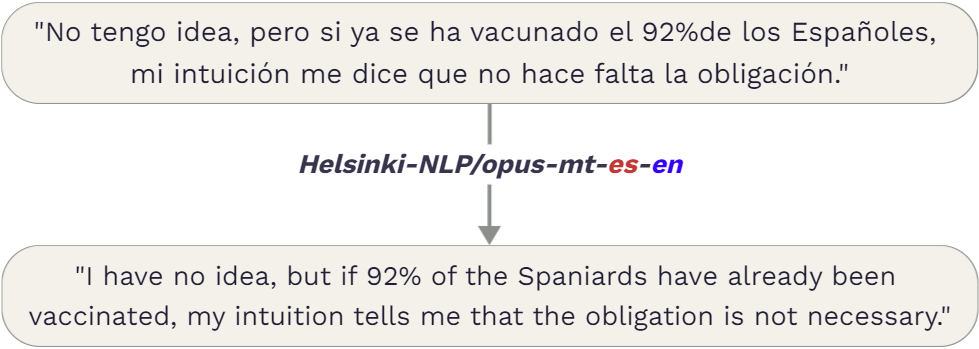
\includegraphics[width=0.75\linewidth, height=0.18\textheight]{Images/trad_es_en.png}
 \caption{\small Example of translation from Spanish to English}
 \label{fig:trad_es_en}
\end{figure}
\FloatBarrier

\begin{figure}[h!]
 \centering
 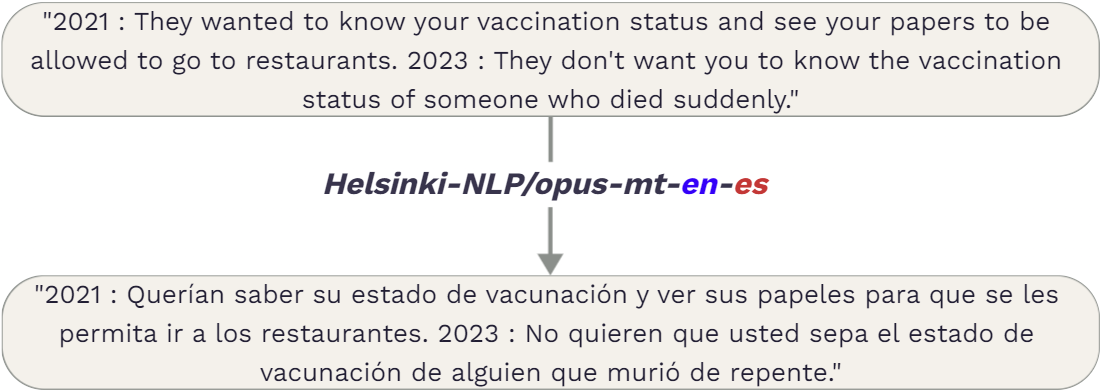
\includegraphics[width=0.78\linewidth, height=0.2\textheight]{Images/trad_en_es.png}
 \caption{\small Example of translation from English to Spanish}
 \label{fig:trad_en_es}
\end{figure}
\FloatBarrier

This strategy was particularly valuable in this context because the Spanish and English datasets were not identical in content, meaning that translating each dataset into the other language provided additional, complementary data rather than just duplicating existing examples. By translating both datasets, the models benefited from more varied training data, which helped to balance the representation of both languages in the model’s learning process.

\section{Data Processing} \label{sec:data_processing_T1}
Data preprocessing and postprocessing were important to prepare raw data for modeling in the case of data preprocessing and refine the model's output, ensuring that the predicted class labels are practical and interpretable, in case of data postprocessing. Together, these processes ensure that binary classification models are trained on high-quality data and produce outputs that are accurate, actionable, and aligned with specific application requirements. The specific techniques and their importance for binary classification will be detailed further in Section \ref{sec:data_preprocessing_T1} for preprocessing and Section \ref{sec:data_postprocessing_T1} for postprocessing.

\subsection{Data Preprocessing} \label{sec:data_preprocessing_T1}
The data preprocessing began with loading the dataset from a JSON file. Next, the labels "CONSPIRACY" and "CRITICAL" were mapped to numerical values (0 and 1). This allows the model to treat the labels as binary classification targets. Then, the model tokenizer broke the text into tokens, applying padding and truncation to ensure uniform input lengths for efficient batch processing.

\subsection{Data Postprocessing} \label{sec:data_postprocessing_T1}
Since we tackled two distinct NLP tasks, each required specific postprocessing steps to ensure that the model outputs conformed to the format required by the organizers. For the binary classification task, a series of detailed procedures were applied to refine the model predictions and store them effectively. The two submitted systems will be explained in Section \ref{sec:systask1}. 

In the first submission, referred to as the conservative approach, we utilized a custom fine-tuned model for sequence classification, along with its associated tokenizer. This step ensured that the model could accurately interpret and classify the input texts. Following the loading of the model and tokenizer, a text classification pipeline was established. This pipeline facilitated the application of the model to the test dataset by managing the tokenization of input texts, processing these texts through the model, and collecting classification results. The pipeline’s automation of these steps ensured efficient processing and consistent handling of the test data.

For the second submission, the experimental approach, we employed three fine-tuned models and their respective tokenizers, each tasked with predicting the category of a given text. After obtaining predictions from all three models, the final category for each document was determined by selecting the label with the highest averaged probability. Finally, these numerical predictions were mapped back to the corresponding labels, either conspiracy or critical.

\section{Systems} \label{sec:systems_T1}
In this section we will describe all the different systems applied in our approach. First would be describe the transformers based approach (Subsection \ref{sec:transformers_based}), then we will explain two different classifiers with different text preprocessing techniques (Subsection \ref{sec:classifiers}), and them we will show all the combination tried in the ensembling approach (Subsection \ref{sec:ensemble_models}).

\subsection{Transformer-based Approach} \label{sec:transformers_based}
The first approach was fine-tuning different transformers models. The process started by ensuring the reproducibility of results, setting a fixed random seed across different components, ensuring that all experimental runs were consistent and produced the same results under identical conditions.

The training procedure was organized using a 3-fold stratified cross-validation setup. Important aspects were the system's ability to dynamically adjust the batch size based on available GPU, the custom learning rate scheduler that gradually reduces the learning rate throughout the training process, as described in details in Section \ref{sec:experiments_setup}. The training process was organized over multiple epochs, and at the end of each epoch, the model's performance was evaluated using a variety of metrics, including accuracy, precision, recall, and F1 score. The results from each fold were written to files, allowing for detailed analysis and comparison across different models or experimental setups. By saving the best-performing model from each fold, the system ensured that the best version of the model is preserved for future use or deployment.

\subsection{Classifiers} \label{sec:classifiers}
We also tried two different classifiers, each coupled with different text preprocessing techniques. The first classifier, referred to as \textit{clf1}, operates using a CountVectorizer to transform raw textual data into a matrix of word counts, where each document is represented by the frequency of its constituent terms. This matrix is then used to train a Multinomial Naive Bayes model, a probabilistic classifier that assumes conditional independence between features. The second classifier, \textit{clf2}, implements a more sophisticated vectorization technique, TF-IDF Vectorizer, which assigns weights to terms based on their frequency in individual documents relative to their appearance across the entire dataset. This approach diminishes the impact of commonly occurring words that offer limited semantic value, while emphasizing rarer, more contextually important terms. Logistic Regression, a discriminative model, is then applied to these weighted features, estimating the likelihood of a document belonging to a particular class based on the learned relationships between words and categories.

Accompanying these classifiers are three different text preprocessing pipelines, each with varying levels of complexity. The simplest approach, referred to as \textit{basic}, converts the text to lowercase, ensuring uniformity across the dataset while retaining punctuation, stop words, and numbers. This method, though computationally light, preserves much of the noise inherent in raw text. The second approach, denoted as \textit{spacy}, leverages the capabilities of the spaCy library to perform advanced linguistic preprocessing \cite{altinok2021mastering}. This includes tokenization, lemmatization, and the removal of stop words and punctuation, allowing the model to focus on the core semantic content of each document by reducing words to their base forms and filtering out irrelevant tokens. In contrast, the third and most complex preprocessing strategy, known as \textit{spacy\_pos}, further refines the input data by applying part-of-speech tagging to retain only tokens belonging to specific grammatical categories, such as nouns, verbs, adjectives, adverbs, and proper nouns. This selective filtering enhances the model's ability to concentrate on syntactically meaningful components of the text.

In order to use classifiers as fine-tuned models within an ensemble, explained in the next subsection, wrapping the classifier was essential for making it reusable and adaptable for different tasks. The wrapping approach used encapsulated the entire process of text preprocessing, feature extraction, and model training into a single, self-contained object. This design allowed the classifier to be treated like any other fine-tuned model. Once wrapped, the classifier could easily be loaded and reused in various parts of the project without having to repeat the setup process. For instance, when used in an ensemble, the classifier takes processed input data and generates predictions that are combined with predictions from other models. The wrapping ensures that all aspects of the classifier’s behavior, from text transformation to prediction generation, are handled within a single interface.

\subsection{Ensemble Models} \label{sec:ensemble_models}
The final approach explored was an ensemble method, where we tried numerous combination of fine-tuned models and classifiers, using both Soft and Hard voting strategies. After loading the models and their respective tokenizers, the dataset was processed in small batches to optimize memory usage. For each batch, the input texts were passed through all three models individually, generating predictions. In soft voting, the prediction for each text consisted of the probability distribution over the two classes. The final prediction for each text was determined by averaging these probabilities across the models, and the class with the highest average probability was selected as the final prediction. In contrast, hard voting operated directly on the predicted categories, instead of averaging probabilities, each model made a categorical prediction. The final prediction for each text was then determined by majority vote. The class predicted by most of the models was chosen.
Once the predictions were aggregated, accuracy, precision, recall and F1-score were calculated. They provided a comprehensive assessment of the model's performance, highlighting the strengths of both voting strategies depending on the task.


\section{Experiments on the Training Dataset} \label{sec:experiments_train_dataset}
In Table \ref{tab:performance_train_en_T1}, we present the results for the English dataset. The second column specifies the number of epochs each model was trained for, while "DA" in the third column stands for "Data Augmented." We represent the first classifier with \textit{clf1} and the second one with \textit{clf2}, each employing different preprocessing techniques: basic, spaCy, or spaCy with part-of-speech tagging (spacy\_pos). Only ensembles involving the second classifiers are reported in the table, as they yielded better results. In the \textit{ensemble-2\_models-1\_clf2}, the two transformer models used were \textit{roberta-base (15 epochs)} and \textit{bert-base-uncased (15 epochs)}, combined with the \textit{clf2-spacy\_pos (DA)} classifier. In the \textit{ensemble-1\_model-2\_clf2}, the transformer model was \textit{roberta-base (15 epochs)}, and the two classifiers involved were \textit{clf2-spacy (DA)} and \textit{clf2-spacy\_pos (DA)}. The abbreviations \textit{HV} and \textit{SV} denote hard voting and soft voting ensemble methods, respectively.

The data shows that transformer-based models, especially ensemble models, generally perform better across key metrics. For instance, the \textit{ensemble-3-models\_SV} achieves the highest accuracy (0.9041), best F1 score (0.9134), and highest precision (0.9223). The \textit{ensemble-3-models\_HV} also performs strongly with an accuracy of 0.9031 and an F1 score of 0.9101. Among the individual transformer models, \textit{roberta-base (15 epochs)} stands out with strong performance, achieving an accuracy of 0.8793 and an F1 score of 0.9072.

Traditional classifiers, such as the \textit{clf2-basic (DA)} model, deliver solid results as well, with an accuracy of 0.884 and an F1 score of 0.886. The performance of \textit{clf2-spacy (DA)} is even better, reaching 0.888 in accuracy and 0.890 in F1 score. These numbers indicate that while traditional classifiers do not outperform the transformer models, they remain competitive, especially when enhanced with spaCy-based preprocessing and data augmentation. Despite their simpler architectures, these classifiers can yield respectable results. The \textit{clf2-spacy (DA)} model, for example, nearly matches some transformer-based models in both accuracy and F1 score. This suggests that with the right enhancements, such as data augmentation and feature engineering, traditional classifiers remain a relevant choice. Their lower computational requirements make them particularly useful when resources are limited or when transformer models are impractical.

Moreover, ensembling the models leads to better results for both transformers and classifiers. This demonstrates that combining the strengths of multiple models, regardless of the underlying architecture, results in stronger overall performance.

%classifier 1 = Multinomial Naive Bayes with CountVectorizer
%classifier 2 = Logistic Regression with TF-IDF Vectorizer

\begin{table}[h]
    \centering
    \renewcommand{\arraystretch}{1.1}
    \small
    %\begin{tabular}{lccccccc}
    \begin{tabular}{l@{\hskip 2pt}c@{\hskip 8pt}c@{\hskip 10pt}c@{\hskip 10pt}c@{\hskip 8pt}c@{\hskip 8pt}c@{\hskip 8pt}c}
        \hline
        \textbf{Model} & \textbf{Epochs} & \textbf{DA} & \textbf{Acc.} & \textbf{F1} & \textbf{F1-macro} & \textbf{Prec.} & \textbf{Recall} \\
        \hline
        scibert\_scivocab\_uncased & 15 & \checkmark & 0.8637 & 0.8973 & 0.8475 & 0.8734 & \textbf{0.9225} \\
        bert-base-uncased & 15 & \checkmark & 0.8688 & 0.9005 & 0.8539 & 0.8813 & 0.9205 \\
        roberta-base & 15 & \checkmark & 0.8793 & 0.9072 & 0.8672 & 0.8994 & 0.9151 \\
        bert-large-uncased & 5 & \checkmark & 0.8631 & 0.8638 & 0.8401 & 0.8645 & 0.8631 \\
        distilbert-base-uncased & 5 & \checkmark & 0.8629 & 0.8637 & 0.8518 & 0.8640 & 0.8633 \\
        distilbert-base-uncased & 3 & \checkmark & 0.7901 & 0.7891 & 0.7730 & 0.7887 & 0.7895 \\
        ensemble-3-models\_HV & - & \checkmark & 0.9031 & 0.9101 & 0.8801 & 0.9181 & 0.9022 \\
        ensemble-3-models\_SV & - & \checkmark & \textbf{0.9041} & \textbf{0.9134} & \textbf{0.8916} & \textbf{0.9223} & 0.9048 \\
        CT-bert & 4 & \checkmark & 0.7701 & 0.7412 & 0.7102 & 0.7507 & 0.7317 \\
        clf1-basic & - &  & 0.846 & 0.881 & 0.831 & 0.875 & 0.887 \\
        clf1-spacy & - &  & 0.849 & 0.846 & 0.831 & 0.845 & 0.847 \\
        clf1-spacy\_pos & - &  & 0.844 & 0.849 & 0.824 & 0.842 & 0.856 \\
        clf2-basic & - &  & 0.848 & 0.844 & 0.821 & 0.856 & 0.844 \\
        clf2-spacy & - &  & 0.865 & 0.848 & 0.844 & 0.863 & 0.854 \\
        clf2-spacy\_pos & - &  & 0.866 & 0.868 & 0.843 & 0.872 & 0.860 \\
        clf1-basic & - & \checkmark & 0.849 & 0.851 & 0.834 & 0.853 & 0.848 \\
        clf1-spacy & - & \checkmark & 0.860 & 0.862 & 0.843 & 0.867 & 0.854 \\
        clf1-spacy\_pos & - & \checkmark & 0.858 & 0.861 & 0.841 & 0.868 & 0.852 \\
        clf2-basic & - & \checkmark & 0.884 & 0.886 & 0.870 & 0.885 & 0.889 \\
        clf2-spacy & - & \checkmark & 0.888 & 0.890 & 0.872 & 0.888 & 0.893 \\
        clf2-spacy\_pos & - & \checkmark & 0.886 & 0.887 & 0.870 & 0.888 & 0.892 \\
        ensemble-3-clf2\_HV & - & \checkmark & 0.720 & 0.725 & 0.612 & 0.743 & 0.724 \\
        ensemble-3-clf2\_SV & - & \checkmark & 0.731 & 0.718 & 0.644 & 0.738 & 0.724 \\
        ensemble-2\_models-1\_clf2\_HV & - & \checkmark & 0.889 & 0.871 & 0.865 & 0.879 & 0.869 \\
        ensemble-2\_models-1\_clf2\_SV & - & \checkmark & 0.885 & 0.867 & 0.861 & 0.870 & 0.865 \\
        ensemble-1\_model-2\_clf2\_HV & - & \checkmark & 0.887 & 0.865 & 0.859 & 0.871 & 0.856 \\
        ensemble-1\_models-2\_clf2\_SV & - & \checkmark & 0.838 & 0.881 & 0.874 & 0.887 & 0.874 \\
        \hline 
    \end{tabular}
    \caption{\small Binary classification models performance metrics for the English train dataset}
    \label{tab:performance_train_en_T1}
\end{table}
\FloatBarrier

Table \ref{tab:performance_train_es_T1} shows the results for the Spanish dataset. As before, only ensembles involving the second classifiers are included in the table. In the \textit{ensemble-2\_models-1\_clf2}, the two transformer models used were \textit{bert-base-spanish-wwm (15 epochs)} and \textit{bertin-roberta-base-spanish (15 epochs)}, combined with the \textit{clf2-spacy\_pos (DA)} classifier. In the \textit{ensemble-1\_model-2\_clf2}, the transformer model was \textit{bert-base-spanish-wwm (15 epochs)}, and the two classifiers involved were \textit{clf2-spacy (DA)} and \textit{clf2-spacy\_pos (DA)}. 

The table highlights that transformer-based models, especially ensemble models, consistently outperform traditional classifiers. The \textit{ensemble-3\_models\_SV} achieves the highest accuracy (0.8971), best F1 score (0.9248), and highest precision (0.9020). The \textit{ensemble-3\_models\_HV} also performs strongly with an accuracy of 0.8802 and an F1 score of 0.9172. These results demonstrate the clear benefit of ensembling. Individual transformer models like \textit{bert-base-spanish-wwm (15 epochs)} and \textit{bsc-bio-ehr-es-pharmaco-ner (15 epochs)} deliver solid performance but are still outshined by the ensemble approaches. 

Traditional classifiers, although generally behind the transformers, perform competitively when enhanced with data augmentation. For example, the \textit{classifier2-spacy (DA)} model achieves an accuracy of 0.896 and an F1 score of 0.885, showing that older methods can still be effective when improved with modern techniques. This suggests that traditional classifiers remain a viable option, especially when computational resources are limited.

\begin{table}[h]
    \centering
    \renewcommand{\arraystretch}{1.1}
    \small
    %\begin{tabular}{lccccccc}
    \begin{tabular}{l@{\hskip 3pt}c@{\hskip 9pt}c@{\hskip 11pt}c@{\hskip 11pt}c@{\hskip 9pt}c@{\hskip 9pt}c@{\hskip 9pt}c}
        \hline
        \textbf{Model} & \textbf{Epochs} & \textbf{DA} & \textbf{Acc.} & \textbf{F1} & \textbf{F1-macro} & \textbf{Prec.} & \textbf{Recall} \\
        \hline
        bertin-roberta-base-spanish    & 15 & \checkmark & 0.8613 & 0.8992 & 0.8384 & 0.8462 & \textbf{0.9593} \\
        bert-base-spanish-wwm          & 15 & \checkmark & 0.8687 & 0.9005 & 0.8539 & 0.8813 & 0.9205 \\
        bsc-bio-ehr-es-pharmaconer     & 15 & \checkmark & 0.8669 & 0.8973 & 0.8542 & 0.8934 & 0.9012 \\
        roberta-base-bne               & 10 & \checkmark & 0.8675 & 0.8674 & 0.8550 & 0.8672 & 0.8675 \\
        roberta-base                   & 5 & \checkmark & 0.8555 & 0.8529 & 0.8369 & 0.8546 & 0.8555 \\
        ensemble-3\_models\_SV         & - & \checkmark & \textbf{0.8971} & \textbf{0.9248} & \textbf{0.8841} & \textbf{0.9020} & 0.9488 \\
        ensemble-3\_models\_HV         & - & \checkmark & 0.8802 & 0.9172 & 0.8798 & 0.8910 & 0.9451 \\
        alberto-base-spanish           & - & \checkmark & 0.8612 & 0.8610 & 0.8428 & 0.8609 & 0.8613 \\
        clf1-basic             & - & - & 0.807 & 0.7945 & 0.784 & 0.792 & 0.797 \\
        clf1-spacy            & - & - & 0.814 & 0.7990 & 0.788 & 0.800 & 0.798 \\
        clf1-spacy\_pos       & - & - & 0.816 & 0.7994 & 0.789 & 0.804 & 0.795 \\
        clf2-basic            & - & - & 0.809 & 0.7886 & 0.774 & 0.805 & 0.773 \\
        clf2-spacy            & - & - & 0.818 & 0.7985 & 0.772 & 0.818 & 0.780 \\
        clf2-spacy\_pos       & - & - & 0.829 & 0.8118 & 0.783 & 0.836 & 0.789 \\
        clf1-basic            & - & \checkmark & 0.871 & 0.8604 & 0.810 & 0.857 & 0.864 \\
        clf1-spacy            & - & \checkmark & 0.870 & 0.8575 & 0.812 & 0.858 & 0.857 \\
        clf1-spacy\_pos       & - & \checkmark & 0.875 & 0.8625 & 0.815 & 0.864 & 0.861 \\
        clf2-basic            & - & \checkmark & 0.877 & 0.886 & 0.861 & 0.891 & 0.881 \\
        clf2-spacy            & - & \checkmark & 0.896 & 0.885 & 0.864 & 0.896 & 0.875 \\
        clf2-spacy\_pos       & - & \checkmark & 0.894 & 0.883 & 0.862 & 0.893 & 0.874 \\
        ensemble-3-clf2\_HV            & - & \checkmark & 0.772 & 0.748 & 0.724 & 0.788 & 0.712 \\
        ensemble-3-clf2\_SV            & - & \checkmark & 0.798 & 0.778 & 0.729 & 0.815 & 0.745 \\
        ensemble-2\_models-1\_clf\_HV & - & \checkmark & 0.818 & 0.799 & 0.734 & 0.831 & 0.771 \\
        ensemble-2\_models-1\_clf\_SV & - & \checkmark & 0.832 & 0.818 & 0.783 & 0.852 & 0.786 \\
        ensemble-1\_model-2\_clf\_HV  & - & \checkmark & 0.820 & 0.803 & 0.749 & 0.836 & 0.773 \\
        ensemble-1\_models-2\_clf\_SV & - & \checkmark & 0.838 & 0.823 & 0.764 & 0.848 & 0.799 \\
        \hline
    \end{tabular}
    \caption{\small Binary classification models performance metrics for the Spanish train dataset}
    \label{tab:performance_train_es_T1}
\end{table}
\FloatBarrier

\section{Submitted Systems for Task 1} \label{sec:systask1}
This section outlines the systems submitted for task 1, which focuses on distinguishing between critical and conspiracy texts. For this task, the general approach involved fine-tuning transformer-based models and applying good data processing, described in Section \ref{sec:data_processing_T1} and data augmentation techniques, described in Section \ref{sec:data_augmentation_T1}. Both English and Spanish datasets were processed similarly. The main difference between Run 1 and Run 2 lies in the method used to make predictions. In Run 1, only the best model checkpoint was used to make predictions while in Run 2, an ensembling method was employed, which combined the predictions from multiple models.

In Run 1, we focused on using the best model checkpoint to make predictions for both English and Spanish datasets. For English, the \textit{facebook/roberta-base}\footnote{\url{https://huggingface.co/FacebookAI/roberta-base}} \cite{Liu2019RoBERTaAR} model was used. This model is known for its robust performance on various NLP tasks. For Spanish, the \textit{dccuchile/bert-base-spanish-wwm-uncased} model was used, which is specifically trained for the Spanish language. 

In Run 2, an ensembling approach was used. 
The general approach involved using a Soft Voting Ensembling method composed of three custom fine-tuned transformer-based models. We selected two well-known transformer models and incorporated a scientific one. The inclusion of a scientific model aimed to better capture the specialized terminology and nuanced discussions related to scientific content and misinformation about COVID-19. We used the following three models for English:
\begin{enumerate}
    \item \textit{facebook/roberta-base}\cite{Liu2019RoBERTaAR}%\footnote{\url{https://huggingface.co/FacebookAI/roberta-base}} \cite{Liu2019RoBERTaAR}
    \item \textit{google/bert-base-uncased}\footnote{\url{https://huggingface.co/google-bert/bert-base-uncased}} 
    \cite{devlin-etal-2019-bert}
    \item \textit{allenai/sciber\_scivocab\_uncased}\footnote{\url{https://huggingface.co/allenai/scibert_scivocab_uncased}} \cite{beltagy-etal-2019-scibert}
\end{enumerate}
% \end{itemize}

For the Spanish dataset, the approach mirrored the English task but involved different custom fine-tuned models suited to the Spanish language that are:
\begin{enumerate}
    \item \textit{dccuchile/bert-base-spanish-wwm-uncased}\cite{CaneteCFP2020}%\footnote{\url{https://huggingface.co/dccuchile/bert-base-spanish-wwm-uncased}} \cite{CaneteCFP2020}
    \item \textit{PlanTL-GOB-ES/bsc-bio-ehr-es-pharmaconer}\footnote{\url{https://huggingface.co/PlanTL-GOB-ES/bsc-bio-ehr-es-pharmaconer}} \cite{carrino2022pretrained}
    \item \textit{bertin-project/bertin-roberta-base-spanish}\footnote{\url{https://huggingface.co/bertin-project/bertin-roberta-base-spanish}} \cite{BERTIN}
\end{enumerate}
% \end{itemize}

\noindent For ensembling, the best checkpoint from each fine-tuned Spanish model was used in a Soft Voting ensemble for predictions. This approach involved combining predictions from multiple models using a Soft Voting ensemble \cite{covid_soft_voting_2022}, which significantly improved the overall accuracy and robustness of the system. The Soft Voting process involves averaging the predicted probabilities of each category from the different models and then making the final prediction based on the highest average probability.

%By integrating the strengths of different models, the ensembling method provided a more reliable and precise set of predictions, ensuring higher performance in distinguishing between critical and conspiracy texts. 

The methods and findings discussed in this chapter provide insights into \textbf{RQ1}, specifically evaluating model performance in distinguishing conspiracy from critical thinking narratives.

%%%%%%%%%%%%%%%%%%%%%%%%%%%%%%%%%%%%%%%%%%%%%%%%%%%%%%%%%%%%%%%%%%%%%%%%%%%%%%%%%%%%%%%%%

\chapter{Span-level Detection of Narrative Elements} \label{chap:token_class_task}
In this chapter, we will provide a detailed account of the experiments conducted for the span-level detection task, beginning with the data augmentation techniques applied to the dataset. This will be followed by the data preprocessing and the comprehensive analysis of the experiments carried out on the train dataset, culminating in a discussion of the models developed and submitted for the competition.

\section{Data Augmentation} \label{sec:data_augmentation_T2}
Also in this case, data augmentation was crucial in improving the performance of the token classification models. In token classification, certain token classes often dominate the dataset, leading to overfitting and skewed predictions. To mitigate this issue, we employed several augmentation strategies aimed at diversifying the dataset while preserving the core semantics of the text. 
 
\subsection{One-way Translation} \label{subsec:translation_T2}
The initial experiment involved using the translated datasets from the binary classification, with the addition of translating also the "span-text" associated with the six distinct span categories. However, we encountered a significant challenge: after translation, the "start\_char" and "end\_char" markers, which denote the beginning and end positions of these spans, no longer corresponded to the precise words in the original text, as well as "start\_token" and "end\_token". This misalignment arose because there isn't a one-to-one match in the length of the characters between the original and translated texts. Consequently, the span annotations became inaccurate, rendering this approach unusable for our purposes.

\subsection{Synonym Replacement} \label{subsec:synonym_T2}
The second approach was using synonym replacement. This technique is very efficient in token classification because it maintains the structure of the input while introducing vocabulary diversity. In tasks where tokens are mapped to specific labels, keeping the same number of words ensures that the start and end token positions remain aligned. This consistency is crucial for avoiding misalignment in token spans, which could lead to incorrect classification.

When synonyms are used while preserving the token count, the model benefits from encountering different words with similar meanings without disrupting the original token structure. This increases the model’s ability to generalize, making it more robust when dealing with variations in natural language. Additionally, synonym translation enriches the dataset by introducing new vocabulary, offering the model a broader context to understand linguistic nuances, without needing adjustments to the underlying tokenization or the training process.

The first trial of synonym replacement was using WordNet from the NLTK library\footnote{\url{https://www.nltk.org/howto/wordnet.html}}. WordNet, a comprehensive lexical database, organizes words into \textit{synsets} that group together words with similar meanings. By accessing these synsets, alternative lemmas (word forms) can be extracted, offering a range of possible replacements for a given word. In this method, words in both the main text and associated span annotations are replaced with randomly selected synonyms from WordNet, generating alternative versions of the original sentences while preserving the core meaning. However, the method does not take into account the specific context of each word, leading to inappropriate or awkward replacements when a word has multiple meanings. In addition this approach was highly conservative, resulting in minimal changes to the text. WordNet's synsets provided only a limited number of suitable synonyms, and as a result, most words in both the main text and span annotations remained unchanged. This conservative nature meant that very few words were substituted, leading to a dataset that was nearly identical to the original. Due to the lack of significant variation introduced by this method, the augmented dataset was essentially a copy of the original, rendering it ineffective for use in further experiments. The intended goal of generating diverse linguistic structures to improve model generalization was not achieved. Consequently, the augmented data could not be used in training, as it offered no meaningful distinction from the original dataset, limiting the overall impact of the augmentation strategy.

The next approach was using spaCy's pre-trained word embeddings \cite{altinok2021mastering}. It begins by loading the \textit{"en\_core\_web\_md"} spaCy model, which includes pre-trained word vectors that allow for the calculation of word similarities. For each word in the dataset’s text, a synonym is identified by comparing its vector representation with those of other words in the vocabulary. A synonym is selected only if it has the same part-of-speech tag as the original word, ensuring that the new word fits grammatically within the context. If no suitable synonym is found, the original word remains unchanged. After modifying the text, the approach checks if the total word count remains the same as the original. If the word count differs, which indicates that the replacement disrupted the sentence structure, that particular item is skipped to maintain consistency. However, the synonym replacement process was very conservative, often leaving many words unchanged due to strict part-of-speech and similarity requirements. Additionally, the process of performing the synonym translation was notably slow, as identifying and replacing synonyms for each word required considerable computational time.
 
The last approach for enhancing the English dataset involved a combination of advanced tools such as spaCy, static word embeddings (word2vec) \cite{mikolov2013distributed}, and Google News word vectors. This strategy began with spaCy parsing the text to segment each word and assigning the appropriate part of speech, creating a structured linguistic base from which to work. Subsequently, the Google News word2vec vectors, which were compiled from a vast array of news articles, provided a rich network of lexical associations. These vectors are specifically the GoogleNews-vectors-negative300 static word embeddings\footnote{\url{https://github.com/mmihaltz/word2vec-GoogleNews-vectors}}, trained on a dataset of 100 billion words from Google News articles. This allowed for the precise identification of synonyms that closely matched the semantic context of the original words, ensuring that replacements were both meaningful and contextually appropriate. The carefully selected synonyms were then integrated into the text, followed by a crucial recalibration of annotations for text spans to ensure the annotations accurately reflected the changes in word positions and meanings, thus preserving the dataset's relevance and usefulness. 

An example of the synonym augmented data for the English dataset is illustrated in Figure \ref{fig:syn_en}.

\begin{figure}[h!]
 \centering
 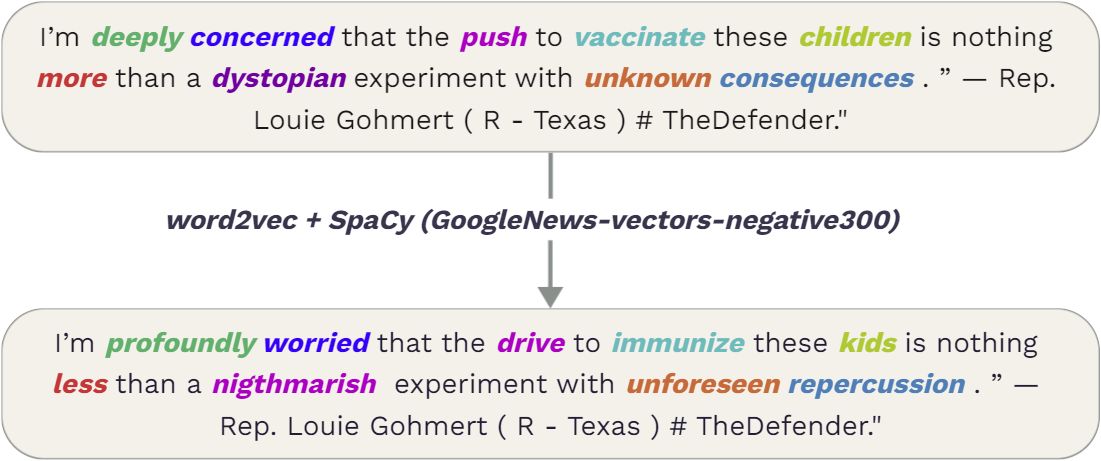
\includegraphics[width=0.79\linewidth, height=0.23\textheight]{Images/syn_en.png}
 \caption{Synonym augmented English dataset example}
 \label{fig:syn_en}
\end{figure}
\FloatBarrier

Building upon the method utilized for the English dataset, a similar approach was adopted for the Spanish dataset, specifically tailored to accommodate the distinct linguistic characteristics of Spanish. This process employed the \textit{"es\_core\_news\_sm"} spaCy model for precise linguistic parsing and syntactic tagging, essential for effective synonym replacement. Further enhancing the approach, \textit{FastText} embeddings from the Spanish Unannotated Corpora\footnote{\url{https://github.com/dccuchile/spanish-word-embeddings}} were integrated. This dataset, in contrast to the Google News vectors, includes a corpus size of 3 billion words and was selected since GoogleNews-vectors were available only for the English dataset. This ensured that the chosen synonyms were contextually appropriate and semantically aligned with the original text.

As with the English process, the Spanish text underwent analysis with the spaCy model to identify grammatical structures, followed by the FastText model's assistance in selecting suitable synonyms for nouns, verbs, adjectives, and adverbs. Special attention was paid to maintain the original intent and readability of the text, carefully avoiding multi-word synonyms that could complicate the narrative flow. Upon integrating the appropriate synonyms, the next critical step involved recalibrating the text's annotations to ensure that they correctly corresponded with the updated text, thus ensuring the annotations remained accurate and relevant for future processing and analysis tasks. An example of the synonym-augmented data for the Spanish dataset is shown in Figure \ref{fig:syn_es}.

\begin{figure}[h!]
 \centering
 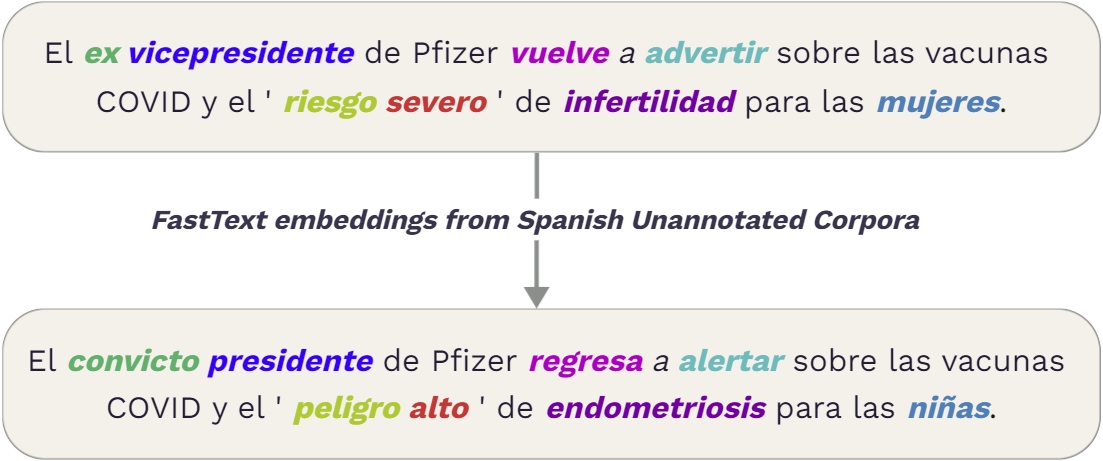
\includegraphics[width=0.79\linewidth, height=0.23\textheight]{Images/syn_es.png}
 \caption{Synonym augmented Spanish dataset example}
 \label{fig:syn_es}
\end{figure}
\FloatBarrier

\section{Data Processing} \label{sec:data_processing_T2}
Data preprocessing and postprocessing are essential for token-classification tasks as they significantly impact model performance and accuracy. Preprocessing involves preparing raw data by applying techniques such as tokenization, stemming, lemmatization, stop word removal, and handling missing values. These steps are critical to ensure that tokens retain the most relevant information while reducing noise, allowing the model to learn more effectively and make precise token-level predictions. Postprocessing, in turn, refines the model’s output by converting predicted labels into meaningful formats, correcting potential errors, and ensuring that results adhere to predefined constraints. This ensures the final output is both interpretable and applicable to real-world tasks. Together, these processes help the model train on high-quality data and produce reliable, actionable outputs. The specific preprocessing techniques will be covered in Section \ref{sec:data_preprocessing_T2}, and postprocessing approaches will be discussed in Subsection \ref{subsec:data_postprocessing_T2}.

\subsection{Data Preprocessing} \label{sec:data_preprocessing_T2}
The preprocessing of data was a critical step in the development of an effective token classification model, used for both the Spanish and English datasets. This section outlines the detailed processes undertaken to transform raw text data into a structured format suitable for model training and evaluation.

\subsubsection{Tokenization and Label Alignment} \label{subsec:tokenization_and_label_alignment_T2}
The first key step was tokenization, where text was broken down into individual tokens (words or subwords). Each sentence in the dataset was tokenized, and the tokenizer generated word IDs to map tokens back to the original words. During this process, the alignment of labels with these tokens was meticulously handled to ensure accurate representation of entities. To align the labels, each token was assigned a corresponding label, considering the start and end positions of the annotated entities. Tokens at the beginning of an entity were marked with a 'B-' (beginning) label, while tokens inside an entity received an 'I-' (inside) label. Tokens not part of any entity were labeled as 'O' (outside). This precise alignment was crucial for maintaining the integrity of the annotations throughout the tokenization process.

\subsubsection{Enhancement of Dataset with Category Columns} \label{subsec:category_oolumn_T2}
To facilitate better data analysis and stratified sampling, binary indicator columns were added for each label category (CAMPAIGNER, VICTIM, AGENT, FACILITATOR, OBJECTIVE, and NEGATIVE\_EFFECT). This involved iterating over the dataset and checking each annotation to determine the presence of specific categories. For each document, a binary column was created for each label, where a value of 1 indicated the presence of the label and 0 indicated its absence. This addition provided a more detailed insight into the distribution of labels across the dataset and was essential for ensuring balanced splits during cross-validation.

\subsubsection{Sentence Preparation and Annotation} \label{subsec:sentence_preparation_T2}
The preparation of sentences and their annotation involved several steps. Each document was divided into sentences. The sentences were then tokenized, and the positions of tokens within the document were recorded. Annotations were mapped to these tokens based on their character offsets in the original text. For each token in a sentence, the corresponding label was determined by checking the overlap of the token’s character range with any annotated spans.

\subsubsection{Data Preparation for Model Training} \label{subsec:data_prepatation_model_training_T2}
For the model training phase, the data was prepared by splitting it into training and evaluation sets for each fold in a stratified k-fold cross-validation setup. This ensured that each fold had a representative distribution of labels. The prepared sentences, now with aligned tokens and labels, were converted into a format suitable to use with the Hugging Face transformers library\footnote{\url{https://huggingface.co/docs/transformers/v4.13.0/index}}. This included creating lists of tokens and their corresponding labels and facilitated efficient data loading and batching during training.

\subsection{Data Postprocessing}\label{subsec:data_postprocessing_T2}
The postprocessing for this task was different from the binary one. After loading the test dataset into a pandas DataFrame\footnote{\url{https://pandas.pydata.org/docs/reference/frame.html}}, the text was segmented into sentences using spacy’s NLP pipeline. The model used for prediction was loaded from a pre-trained directory, and a pipeline was created to handle the token classification task. The pipeline processes the text and generated predictions for each token, including entity labels and confidence scores. However, the predictions were made at the token level, meaning that the raw outputs represented individual tokens rather than entire entities, which may span multiple tokens.

If a sentence exceeded the model’s maximum token length, It was truncated to fit within the allowed token length. This is implemented in the code by checking the length of the sentence and slicing it accordingly. The pipeline then made predictions on the truncated text, ensuring that the model could process the input within its constraints. Once the pipeline generated token-level predictions, the next step was to aggregate these predictions into meaningful entity spans. The model's predictions included start and end positions for each token within the sentence, but these positions must be mapped back to the original text. This was done by adjusting the token offsets relative to the start of the sentence. These adjustments ensured that each token’s prediction aligns with its position in the original document. The code also handled cases where multiple tokens were part of the same entity. For example, if the entity "COVID - 19 pandemic" was predicted, each word may have received an individual prediction. In the postprocessing step, predictions were merged into a single entity span by aggregating the start and end positions of related tokens and optionally averaging their confidence scores. This aggregation ensures that multi-token entities are represented as single, cohesive spans in the final output.

\section{Systems} \label{sec:system_T2}
The methodology involves fine-tuning a pre-trained transformer model for token classification, specifically using a BIO tagging scheme for entity recognition. The process begins by setting the environment and configuring parameters for optimal resource usage. Ensuring reproducibility is a priority, and this is achieved by setting a random seed, which guarantees that all processes depending on random operations yield consistent results across different runs. A key component of the approach is adjusting the batch size dynamically according to the available GPU memory. This dynamic adjustment ensures that the training process can handle memory constraints efficiently without causing interruptions, as described in Section \ref{sec:experiments_setup}. Then all the data preprocessing is done as explained in Section \ref{sec:data_preprocessing_T2}. %To ensure robust model training, stratified k-fold cross-validation is employed, as already explained in Section \ref{sec:experiments_setup}. 

During training, a custom learning rate scheduler is employed to adjust the learning rate dynamically over time. For each fold, the model is trained using the HuggingFace Trainer class. Metrics such as precision, recall, F1 score, and accuracy are computed using the seqeval library\footnote{\url{https://pypi.org/project/seqeval/1.2.2/}}, which is designed for sequence labeling tasks. After training and evaluating the model for all folds, the metrics are averaged across all folds to provide a summary of the model’s performance. This averaging step is used solely to gauge the model's overall performance. Finally, the best model checkpoint from cross-validation, based on these performance metrics, is selected and evaluated on the test dataset to provide a final assessment of the model's effectiveness.  This cross-validation approach ensures that the model's evaluation metrics are reliable and that the model generalizes well to unseen data. Throughout the process, results are saved to files for further analysis, and necessary directories are created to store the outputs. This methodology ensures that the training process is both efficient and scalable, while also providing robust evaluation through cross-validation. 

\section{Experiments on the Training Dataset} \label{sec:experiments_train_dataset_T2}

Table \ref{tab:performance_train_en_T2} presents the results for the English dataset. The second column indicates the number of training epochs for each model, with all models trained using data augmentation. The performance of the token classification models in the table reveals notable differences in how each model approaches the task. \textit{roberta-base (15 epochs)} achieves the highest accuracy (0.8897), but its F1 score of 0.5890 indicates a slight imbalance. This model has a better recall (0.6112) than precision (0.5684), meaning it tends to identify more tokens, though it sacrifices precision, suggesting a higher likelihood of false positives. Models such as \textit{distilbert-base-uncased (15 epochs)} and \textit{bert-base-uncased (15 epochs)} follow closely. Their higher recall compared to precision suggests they prioritize identifying more tokens, even if it results in some misclassifications. This trend is common in models focused on maximizing token identification.

\begin{table}[H]
    \centering
    %\small
    \begin{tabular}{lcccccc}
        \hline
        \textbf{Model} & \textbf{Epochs} & \textbf{Accuracy} & \textbf{F1} & \textbf{Precision} & \textbf{Recall} \\
        \hline
        roberta-base & 15 & \textbf{0.8897} & \textbf{0.5890} & \textbf{0.5684} & \textbf{0.6112} \\
        roberta-base & 10 & 0.8210 & 0.4212 & 0.3943 & 0.4520 \\
        distilbert-base-uncased & 5 & 0.6932 & 0.2881 & 0.2893 & 0.2869 \\  
        distilbert-base-uncased & 10 & 0.8457 & 0.4551 & 0.4279 & 0.4860 \\  
        distilbert-base-uncased & 15 & 0.8563 & 0.5645 & 0.5388 & 0.5928 \\  
        bert-base-uncased & 15 & 0.8723 & 0.5278 & 0.4976 & 0.5619 \\  
        dmis-lab/biobert-v1.1 & 15 & 0.8439 & 0.4608 & 0.4353 & 0.4894 \\  
        dslim/bert-base-NER & 12 & 0.7578 & 0.3412 & 0.2928 & 0.4088 \\
        xlnet-base-cased & 15 & 0.8856 & 0.5716 & 0.5522 & 0.5924 \\
        covid-twitter-bert & 4 & 0.7401 & 0.3301 & 0.3279 & 0.3323 \\
        \hline 
    \end{tabular}
    \caption{\small Token classification models performance metrics for the English dataset}
    \label{tab:performance_train_en_T2}
\end{table}

\begin{table}[H]
    \centering
    %\small
    \begin{tabular}{lcccccc}
        \hline
        \textbf{Model} & \textbf{Epochs} & \textbf{Accuracy} & \textbf{F1} & \textbf{Precision} & \textbf{Recall} \\
        \hline
        facebook/roberta-base & 15 & \textbf{0.8897} & \textbf{0.5890} & \textbf{0.5684} & \textbf{0.6112} \\
        facebook/roberta-base & 10 & 0.8210 & 0.4212 & 0.3943 & 0.4520 \\
        distilbert-base-uncased & 5 & 0.6932 & 0.2881 & 0.2893 & 0.2869 \\  
        distilbert-base-uncased & 10 & 0.8457 & 0.4551 & 0.4279 & 0.4860 \\  
        distilbert-base-uncased & 15 & 0.8563 & 0.5645 & 0.5388 & 0.5928 \\  
        bert-base-uncased & 15 & 0.8723 & 0.5278 & 0.4976 & 0.5619 \\  
        dmis-lab/biobert-v1.1 & 15 & 0.8439 & 0.4608 & 0.4353 & 0.4894 \\  
        dslim/bert-base-NER & 12 & 0.7578 & 0.3412 & 0.2928 & 0.4088 \\
        xlnet-base-cased & 15 & 0.8856 & 0.5716 & 0.5522 & 0.5924 \\
        covid-twitter-bert & 4 & 0.7401 & 0.3301 & 0.3279 & 0.3323 \\
        \hline 
    \end{tabular}
    \caption{\small Token classification models performance metrics for the English dataset}
    \label{tab:performance_train_en_T2}
\end{table}

In Table \ref{tab:performance_train_es_T2}, we present the results for the Spanish dataset. 

As before, the number of training epochs is included in the second column. The performance of the token classification models demonstrates significant differences in how effectively they handle the task. The model \textit{PlanTL-GOB-ES/roberta-base-bne (15 epochs)} stands out with the highest accuracy (0.9326) and a balanced F1 score of 0.5849. Its precision (0.5833) and recall (0.5866) are closely aligned, indicating that it performs consistently in identifying and classifying tokens. The model \textit{Bertin-roberta-base-spanish (12 epochs)} shows similar F1 scores but slightly lower accuracy, with a well-balanced precision and recall. Other models, such as \textit{PlanTL-GOB-ES/roberta-base-bne (8 epochs)} and \textit{bert-base-spanish-wwm-uncased (10 epochs)}, display lower F1 scores, illustrating that fewer training epochs negatively impact their ability to generalize. In contrast, \textit{distilbert-base-spanish-uncased (15 epochs)} offers an intriguing result with a relatively high F1 score (0.5101), showing that compact models can still perform competitively. 

\begin{table}[H]
    \centering
    %\small
    \begin{tabular}{lccccc}
        \hline
        \textbf{Model} & \textbf{Epochs} & \textbf{Accuracy} & \textbf{F1} & \textbf{Precision} & \textbf{Recall} \\
        \hline
        PlanTL-GOB-ES/roberta-base-bne  & 15 & \textbf{0.9326} & \textbf{0.5849} & \textbf{0.5833} & \textbf{0.5866} \\
        PlanTL-GOB-ES/roberta-base-bne  & 8  & 0.9011 & 0.4565 & 0.4562 & 0.4568 \\  
        bert-base-spanish-wwm-uncased   & 10 & 0.8213 & 0.4201 & 0.4093 & 0.4315 \\  
        bertin-roberta-base-spanish     & 12 & 0.8598 & 0.5844 & 0.5856 & 0.5832  \\ 
        alberto-base-spanish            & 8 & 0.7841 & 0.3841 & 0.3833 & 0.3848 \\  
        distilbert-base-spanish-uncased & 15 & 0.8047 & 0.5101 & 0.5019 & 0.5185  \\ 
        electra-small-spanish           & 5 & 0.7288 & 0.3421 & 0.3332 & 0.3513  \\  
        xlm-roberta-base                & 5 & 0.7981 & 0.4012 & 0.3834 & 0.4206  \\ 
        \hline 
    \end{tabular}
    \caption{\small Token classification models performance metrics for the Spanish dataset}
    \label{tab:performance_train_es_T2}
\end{table}
\FloatBarrier


\section{Submitted Systems for Task 2} \label{sec:systask2}
In this section, we describe our submitted systems for detecting elements of oppositional narratives (task 2). We approached task 2 by fine-tuning a transformer model, using also strong data processing, described in Section \ref{sec:data_processing_T2}, and data augmentation, described in Section \ref{sec:data_augmentation_T2}.  We treated task 2 as a token classification problem by fine-tuning models with a single token classification head. Having only one head (instead of a classification head per label, as implemented in the provided baseline \cite{korencic2024oppositional}) precluded the possibility of overlapping spans, but offered increased simplicity and reduced computational expense instead.
While the provided data was annotated at the document-level, we transformed it so that we could train the token classifier at the sentence-level instead. Segmenting the text into sentences overcame the problem of transformers truncating texts that are longer than the maximum length size, ensuring no data was lost during training or testing. 

In the first submitted run, we applied the best model checkpoint without additional training. For the English dataset the \textit{facebook/roberta-base}%\footnote{\url{https://huggingface.co/FacebookAI/roberta-base}} \cite{Liu2019RoBERTaAR}
model was employed while for the Spanish dataset, the \textit{PlanTL-GOB-ES/roberta-base-bne}\footnote{\url{https://huggingface.co/PlanTL-GOB-ES/roberta-base-bne}} \cite{gutierrez2022maria} model was used. 

For the second run, the best model checkpoint from the first run was trained for one more epoch using the augmented dataset as train, without having any data for validation. This final model checkpoint was then used to detect the elements of oppositional narratives in the test dataset. 

The span-detection techniques described here directly address \textbf{RQ2}, exploring the feasibility and challenges of identifying narrative elements in multilingual datasets.

%%%%%%%%%%%%%%%%%%%%%%%%%%%%%%%%%%%%%%%%%%%%%%%%%%%%%%%%%%%%%%%%%%%%%%%%%%%%%%%%%%%%%%%%%%%%%%%%%%%%


\chapter{Results on the Test Dataset} \label{chap:results_test_dataset}
The official evaluation metrics were different for each task. For the binary classification task, the Matthews Correlation Coefficient was used as the primary evaluation metric \cite{chicco2020advantages}, while for the span-level detection task, the macro-averaged span-F1 \cite{da2020semeval} score was employed. In addition to these primary metrics, binary F1 scores for each class were provided for task 1, and per-category span-F1 scores were reported for task 2.

\noindent The shared task organizers provided two hard baseline models for these tasks. For task 1, the baseline is a standard BERT classifier \cite{devlin-etal-2019-bert}. For task 2, the baseline is a BERT-based multi-task token classifier with separate classification heads and a common transformer backbone. 

The baselines utilize either English or Spanish BERT models, depending on the language. The performances of our approaches and the baselines are reported in Table \ref{tab:subtask1_results} (task 1) and in Table \ref{tab:subtask2_results} (task 2). The complete official ranking \cite{korencic2024oppositional} for the English dataset can be found in Table \ref{tab:task1_results_en_full}, while the Spanish official ranking can be found in Table \ref{tab:task1_results_es_full}.


\begin{table}[H]
\centering
\begin{tabular}{lcccc}
\hline
        & \multicolumn{4}{c}{Task 1} \\
        & \textbf{MCC}                & \textbf{F1-macro}           & \textbf{F1-conspiracy}     & \textbf{F1-critical} \\
\hline
\textbf{\textit{English\_baseline}}  & \textit{0.7964} & \textit{0.8975} & \textit{0.8632} & \textit{0.9318} \\ 
\textbf{English\_submitted\_run1} & 0.7574 & 0.8769 & 0.8338 & 0.9200 \\ 
\textbf{English\_submitted\_run2} & 0.7872 & 0.8917 & 0.8536 & 0.9297 \\ 
\hline
\textbf{\textit{Spanish\_baseline}}  & \textit{0.6681} & \textit{0.8339} & \textit{0.7872} & \textit{0.8806} \\ 
\textbf{Spanish\_submitted\_run1} & 0.6147 & 0.7950 & 0.7179  & 0.8720 \\ 
\textbf{Spanish\_submitted\_run2} & 0.6722  & 0.8293 & 0.7699 & 0.8887  \\
\hline
\end{tabular}
\caption{Performance metrics results for task 1}
\label{tab:subtask1_results}
\end{table}
\FloatBarrier

\begin{table}[H]
\centering
\begin{tabular}{lcccc}
\hline
& \multicolumn{4}{c}{Task 2} \\
& \textbf{span-P}                & \textbf{span-R}           & \textbf{span-F1}      & \textbf{micro-span-F1}  \\
\hline
\textbf{\textit{English\_baseline}} & \textit{0.5323} & \textit{0.4684} & \textit{0.6334} & \textit{0.4998} \\ 
\textbf{English\_submitted\_run1} & 0.5832 & 0.6856 & 0.6293 & 0.6074 \\ 
\textbf{English\_submitted\_run2} & 0.5859 & 0.6790 & 0.6279 & 0.6120 \\ 
\hline
\textbf{\textit{Spanish\_baseline}}  & \textit{0.4533} & \textit{0.5621} & \textit{0.4934} & \textit{0.4952} \\
\textbf{Spanish\_submitted\_run1} & 0.5997 & 0.6193 & 0.6089  & 0.6051 \\ 
\textbf{Spanish\_submitted\_run2} & 0.6159 & 0.6129 & 0.6129  & 0.6108 \\ 
\hline
\end{tabular}
\caption{Performance metrics results for task 2}
\label{tab:subtask2_results}
\end{table}
\FloatBarrier % Ensures that the tables are placed before this point

\section{Discussion} \label{sec:discussion}
This section analyzes the results presented in Tables \ref{tab:subtask1_results} and \ref{tab:subtask2_results}. We will provide insights into the results for both English and Spanish datasets, considering the baselines provided by the shared task organizers and how our approaches performed \cite{tulbure2024conspiracy}. We organize this discussion by task and language. First, we examine the binary classification results from task 1. We then turn our attention to task 2.

\subsection{Task 1: Binary Classification} \label{subsec:subtask1_discussion}
We begin by examining the English dataset results, followed by a focused analysis of the Spanish dataset to assess language-specific performance.
\subsubsection{English Results in Task 1} \label{subsubsec:en_res_T1}
In our analysis of the English dataset, the first submitted run exhibited good performance metrics. The Matthews Correlation Coefficient was 0.7574, indicating a robust ability to distinguish between different narrative types. The F1-macro score of 0.8769 further supported the model's high overall classification capability. Notably, the F1 score for critical thinking texts was 0.9200, compared to 0.8338 for conspiracy texts. This disparity suggests that the model more effectively identified critical thinking, potentially due to the more nuanced nature of conspiracy texts. However, it is important to note that these results are below the baseline, which had an MCC of 0.7964 and an F1-macro score of 0.8975. This baseline is indeed a hard baseline and difficult to beat.

In the second submitted run, the model demonstrated improved reliability, with the MCC rising to 0.7872. The F1-macro score also increased to 0.8917, indicating enhanced overall performance. The F1 scores for conspiracy and critical texts were 0.8536 and 0.9297, respectively, showing more balanced and accurate classifications. Despite these improvements, the model still did not surpass the baseline, highlighting the baseline's strong performance and the challenges in achieving higher accuracy.

\subsubsection{Spanish Results in Task 1} \label{subsubsec:es_res_T1}
For the Spanish dataset, the first submitted run showed moderate performance with an MCC of 0.6147, indicating the need for further improvement. The F1-macro score was 0.795, reflecting decent overall performance but highlighting areas for enhancement. The model struggled more with conspiratorial texts, achieving an F1 score of 0.7179 for conspiracy versus 0.8720 for critical texts, likely due to the specific linguistic challenges presented by the Spanish language. The baseline for Spanish had an MCC of 0.6681 and an F1-macro score of 0.8339, indicating that the baseline was also strong for this language.

In the second submitted run, there was a noticeable improvement in performance. The MCC increased to 0.6722, and the F1-macro score rose to 0.8293, indicating better overall performance. The F1 scores for conspiracy and critical texts improved significantly to 0.7699 and 0.8887, respectively. These improvements suggest that the model became more adept at handling linguistic features specific to Spanish, leading to more balanced and accurate classifications. This second run beat the strong baseline performance, reflecting significant progress.

\subsection{Task 2: Span-level Detection} \label{subsec:subtask2_discussion}
We start with span detection results for English, then we explore the model's effectiveness in identifying narrative elements in Spanish.

\subsubsection{English Results in Task 2} \label{subsubsec:en_res_T2}
In the first submitted run for the English dataset, the model achieved a span-P of 0.5832 and a span-R of 0.6856, indicating moderate precision but better recall. The span-F1 score was 0.6293, and the micro-span-F1 score was 0.6074, suggesting a balanced performance with a need for improvement in precision. The baseline for this task had a span-F1 score of 0.6334 and a micro-span-F1 of 0.4998, showing that our model performed significantly better in terms of micro-span-F1 but slightly underperformed in span-F1 compared to the strong baseline.

In the second submitted run, there was a slight improvement in precision, with a span-P of 0.5859 and a span-R of 0.6790. The span-F1 score remained relatively consistent at 0.6279, and the micro-span-F1 score increased marginally to 0.6120. These modest enhancements reflect steady progress in performance and show that our model maintained competitive performance with the baseline.

\subsubsection{Spanish Results in Task 2} \label{subsubsec:es_res_T2}
For the Spanish dataset, the first submitted run demonstrated a balanced performance, with a span-P of 0.5997 and a span-R of 0.6193. The span-F1 score was 0.6089, and the micro-span-F1 score was 0.6051. The model performed significantly better at span detection in Spanish compared to English, possibly due to distinct narrative markers in the language. The baseline for this task had a span-F1 score of 0.4934 and a micro-span-F1 of 0.4952, indicating that our model significantly outperformed the baseline in both metrics.

In the second submitted run, the performance improved, with a span-P of 0.6159, a span-R of 0.6129, and a span-F1 of 0.6129. These stable scores reflect consistent and reliable performance in detecting narrative elements at the span level, maintaining a significant advantage over the baseline.

Due to the best performances obtained in both English and Spanish for the second task, our model achieved the highest overall scores, leading to the first-place ranking in the shared task competition \cite{tulbure2024conspiracy}. Overall, the consistent improvement across both tasks and languages in the second submitted run underscores the effectiveness of the adjustments made in data augmentation, training processes, and model parameter tuning. %These enhancements have contributed to more reliable, balanced, and accurate model performance in both classifying narratives and detecting narrative elements.

\section{Analysis with and without Data Augmentation} \label{sec:analysis_with_without_data_aug}
Table \ref{tab:performance_test_with_without_data_aug_T1} and Table \ref{tab:performance_test_with_without_data_aug_T2} present a comparative analysis of the submitted fine-tuned models with and without data augmentation using the test datasets. For task 1, the results demonstrate that models incorporating data augmentation consistently outperform those without it across all metrics and in both languages. This is especially evident in the MCC and F1-macro scores. For example, in \textit{run1 (English)}, the MCC increased from 0.6880 without augmentation to 0.7574 with it, while the F1-macro score improved from 0.8344 to 0.8769. Notable gains are also observed in the F1-Conspiracy and F1-Critical scores, indicating that data augmentation enhances the model's ability to capture both conspiracy and critical thinking narrative elements more effectively. A similar trend is observed in \textit{run1 (Spanish)}, with the MCC rising from 0.5740 without augmentation to 0.6148 with it. Although the improvement is less pronounced in \textit{run2 (English)} and \textit{run2 (Spanish)}, data augmentation still results in marginal gains, underscoring its value even in more optimized runs. The performance boost observed for both English and Spanish datasets suggests that the data augmentation strategy is robust across languages. These findings highlight the effectiveness of data augmentation in enhancing span-based performance across different languages.

In Figures \ref{fig:T1_grouped_bar_chart} and \ref{fig:T2_grouped_bar_chart}, we can observe that experiments with data augmentation yield better results across all metrics. The dotted lines in these figures represent the experiments without data augmentation, while the solid colored blocks indicate those with data augmentation.

\begin{figure}[h]
 \centering
 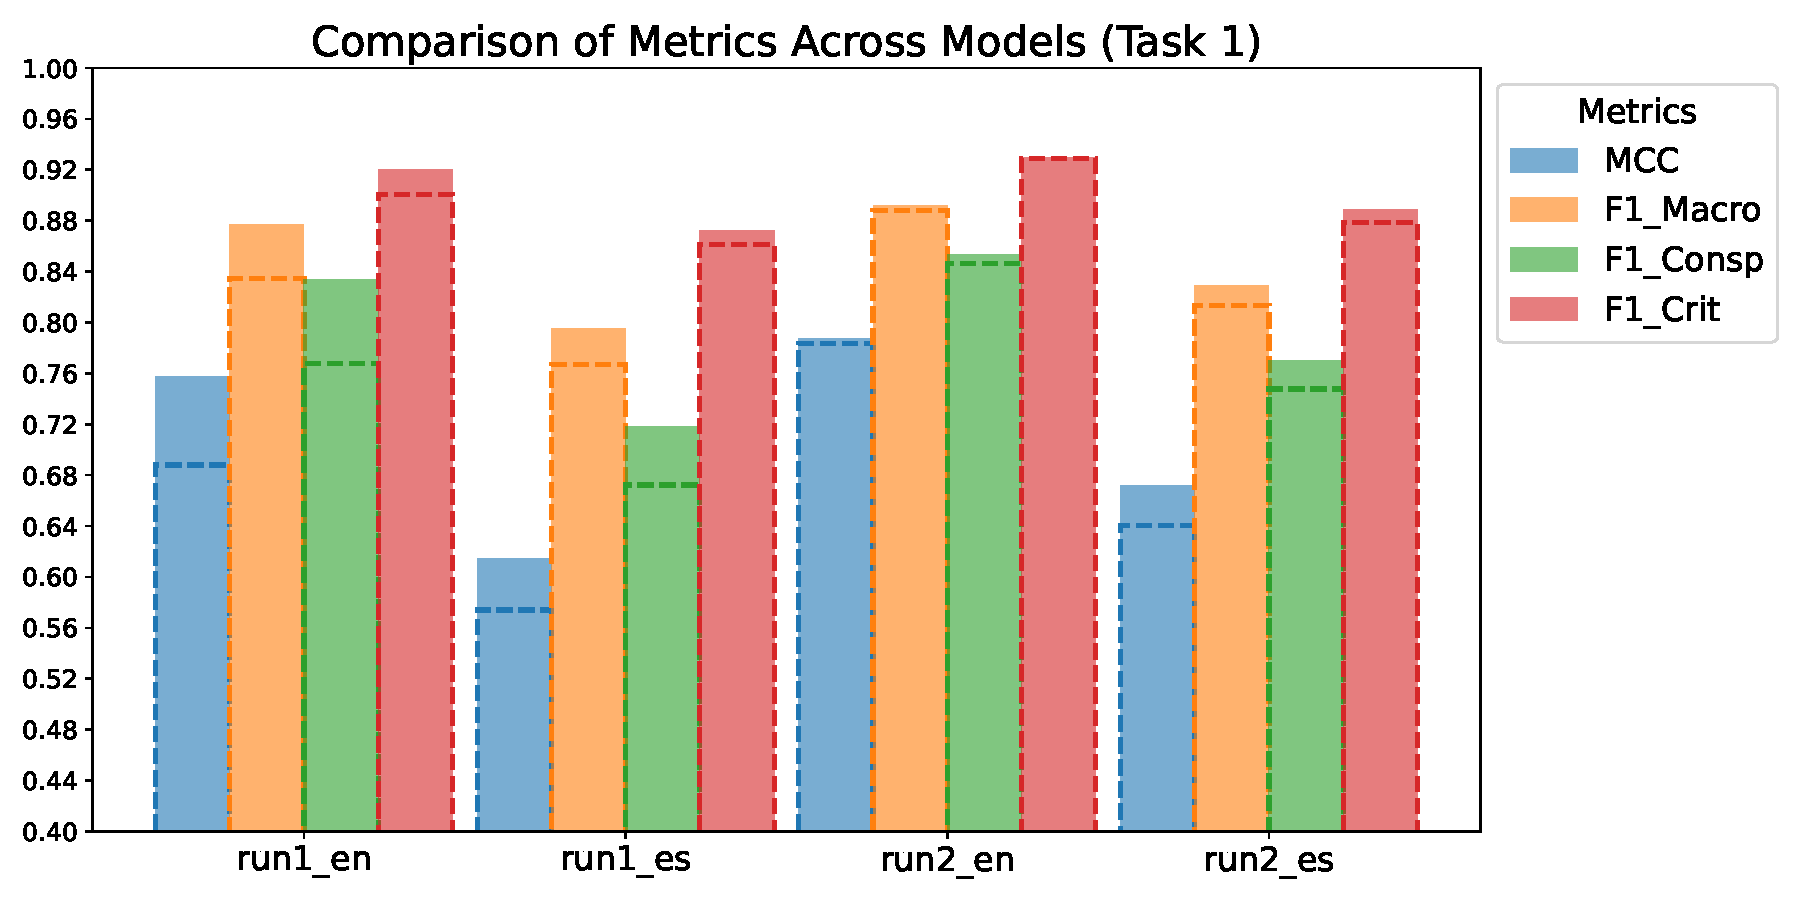
\includegraphics[width=0.92\linewidth, height=0.30\textheight]{Images/task1_bar_plot_comparison_adjusted_v2.pdf}
 \caption{Task 1 metrics comparison with and without data augmentation}
 \label{fig:T1_grouped_bar_chart}
\end{figure}
\FloatBarrier


\begin{table}[h]
    \centering
    \small
    \begin{tabular}{lcccccc}
        \hline
        \textbf{Model} & \textbf{Data Aug} & \textbf{MCC} & \textbf{F1-Macro} & \textbf{F1-Consp} & \textbf{F1-Crit} \\
        \hline
        \multicolumn{6}{c}{\textbf{ENGLISH}} \\
        \hline
        run1 & \checkmark & 0.7574 & 0.8769 & 0.8338 & 0.9200 \\ 
        run1 &            & 0.6880 & 0.8344 & 0.7679 & 0.9008 \\ \hline
        run2 & \checkmark & 0.7872 & 0.8917 & 0.8536 & 0.9297 \\ 
        run2 &            & 0.7836 & 0.8877 & 0.8463 & 0.9291 \\ 
        \hline
        \multicolumn{6}{c}{\textbf{SPANISH}} \\
        \hline
        run1 & \checkmark & 0.6148 & 0.7950 & 0.7179 & 0.8721 \\ 
        run1 &            & 0.5740 & 0.7667 & 0.6723 & 0.8612 \\ \hline
        run2 & \checkmark & 0.6722 & 0.8293 & 0.7699 & 0.8887 \\ 
        run2 &            & 0.6402 & 0.8131 & 0.7477 & 0.8785 \\ 
        \hline 
    \end{tabular}
    \caption{Evaluation metrics with and without data augmentation for task 1}
    \label{tab:performance_test_with_without_data_aug_T1}
\end{table}
\FloatBarrier


For task 2, the benefits of data augmentation remain positive, though they are more subtle compared to task 1. For example, in \textit{run1 (English)}, the span-F1 score increases from 0.6180 without augmentation to 0.6404 with it. Similarly, for \textit{run2 (English)}, span-F1 rises from 0.6087 to 0.6279 with data augmentation. The precision and recall values show consistent improvements as well, suggesting that data augmentation enhances the model's ability to correctly identify and classify narrative spans while maintaining a balanced precision-recall tradeoff. In Spanish, the span-F1 improvement is also evident, such as in \textit{run1 (Spanish)}, where it goes from 0.6010 to 0.6215, and in \textit{run2 (Spanish)}, where it increases from 0.5998 to 0.6232. 


\begin{figure}[h]
 \centering
 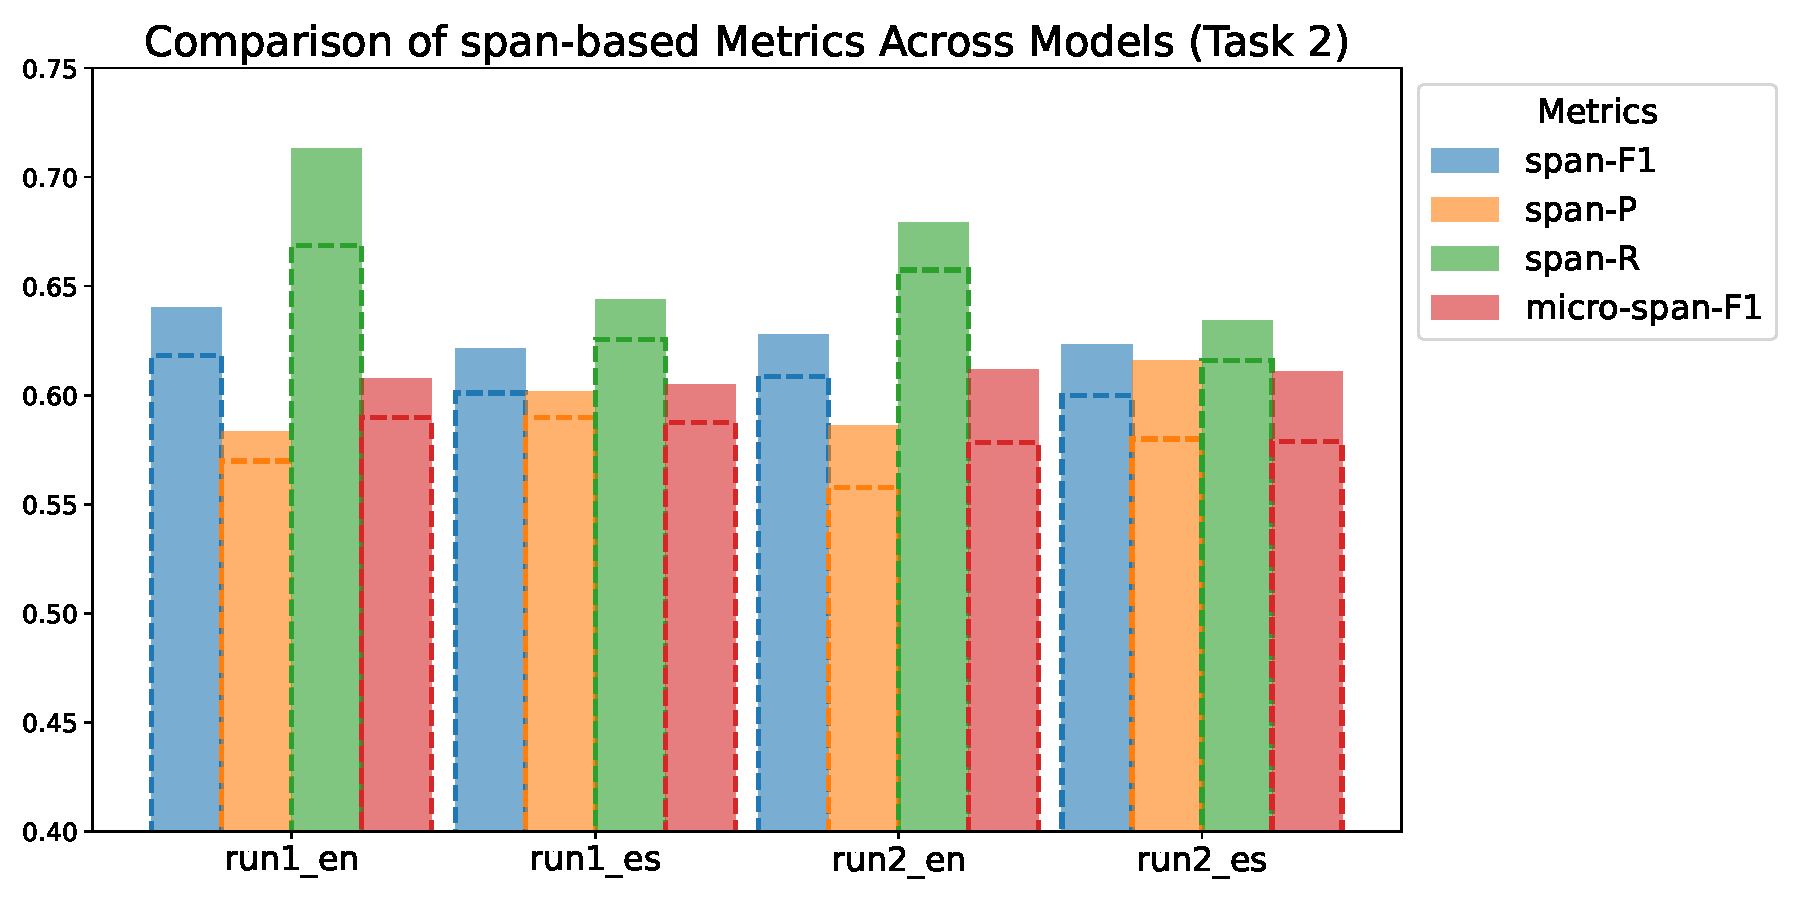
\includegraphics[width=0.92\linewidth, height=0.30\textheight]{Images/task2_bar_plot_comparison_adjusted.pdf}
 \caption{Task 2 metrics comparison with and without data augmentation}
 \label{fig:T2_grouped_bar_chart}
\end{figure}
\FloatBarrier

\begin{table}[h]
    \centering
    \small
    \begin{tabular}{lccccc}
        \hline
        \textbf{Model} & \textbf{Data Aug} & \textbf{span-F1} & \textbf{span-P} & \textbf{span-R} & \textbf{micro-span-F1} \\
        \hline
        \multicolumn{6}{c}{\textbf{ENGLISH}} \\
        \hline
        run1 & \checkmark & 0.6404 & 0.5832 & 0.7133 & 0.6077 \\ 
        run1\ & & 0.6180 & 0.5698 & 0.6687 & 0.5897 \\ 
        \hline
        run2 & \checkmark & 0.6279 & 0.5859 & 0.6790 & 0.6120 \\ 
        run2 & & 0.6087 & 0.5578 & 0.6574 & 0.5784 \\ 
        \hline
        \multicolumn{6}{c}{\textbf{SPANISH}} \\
        \hline
        run1 & \checkmark & 0.6215 & 0.6015 & 0.6438 & 0.6051 \\ 
        run1 & & 0.6010 & 0.5897 & 0.6257 & 0.5874 \\ 
        \hline
        run2 & \checkmark & 0.6232 & 0.6159 & 0.6342 & 0.6108 \\ 
        run2 & & 0.5998 & 0.5799 & 0.6158 & 0.5787 \\ 
        \hline 
    \end{tabular}
    \caption{Evaluation metrics with and without data augmentation for task 2}
    \label{tab:performance_test_with_without_data_aug_T2}
\end{table}
\FloatBarrier


The findings presented in this section provide clear insights into \textbf{RQ3}, demonstrating that specific data augmentation techniques, such as back-translation and synonym replacement, have a measurable impact on model performance. This analysis highlights the role of augmentation in improving the model's ability to handle diverse and complex narrative structures across multilingual datasets.

%%%%%%%%%%%%%%%%%%%%%%%%%%%%%%%%%%%%%%%%%%%%%%%%%%%%%%%%%%%%%%%

\chapter{Error Analysis} \label{chap:error_analysis}
In this section, we analyze the performance of our submitted models. The error analysis enables us to understand where the model's predictions diverge from the actual categories. 

\section{Task 1: Binary Classification}
We begin by examining the confusion matrix of the binary classification task, which provides a visual representation of the model's performance by illustrating the frequency of correct predictions for each category and the frequency of misclassifications.

\begin{figure}[H]
    \centering
    \subfloat[Confusion matrix for the English dataset\label{fig:confusion_matrix_english}]{
        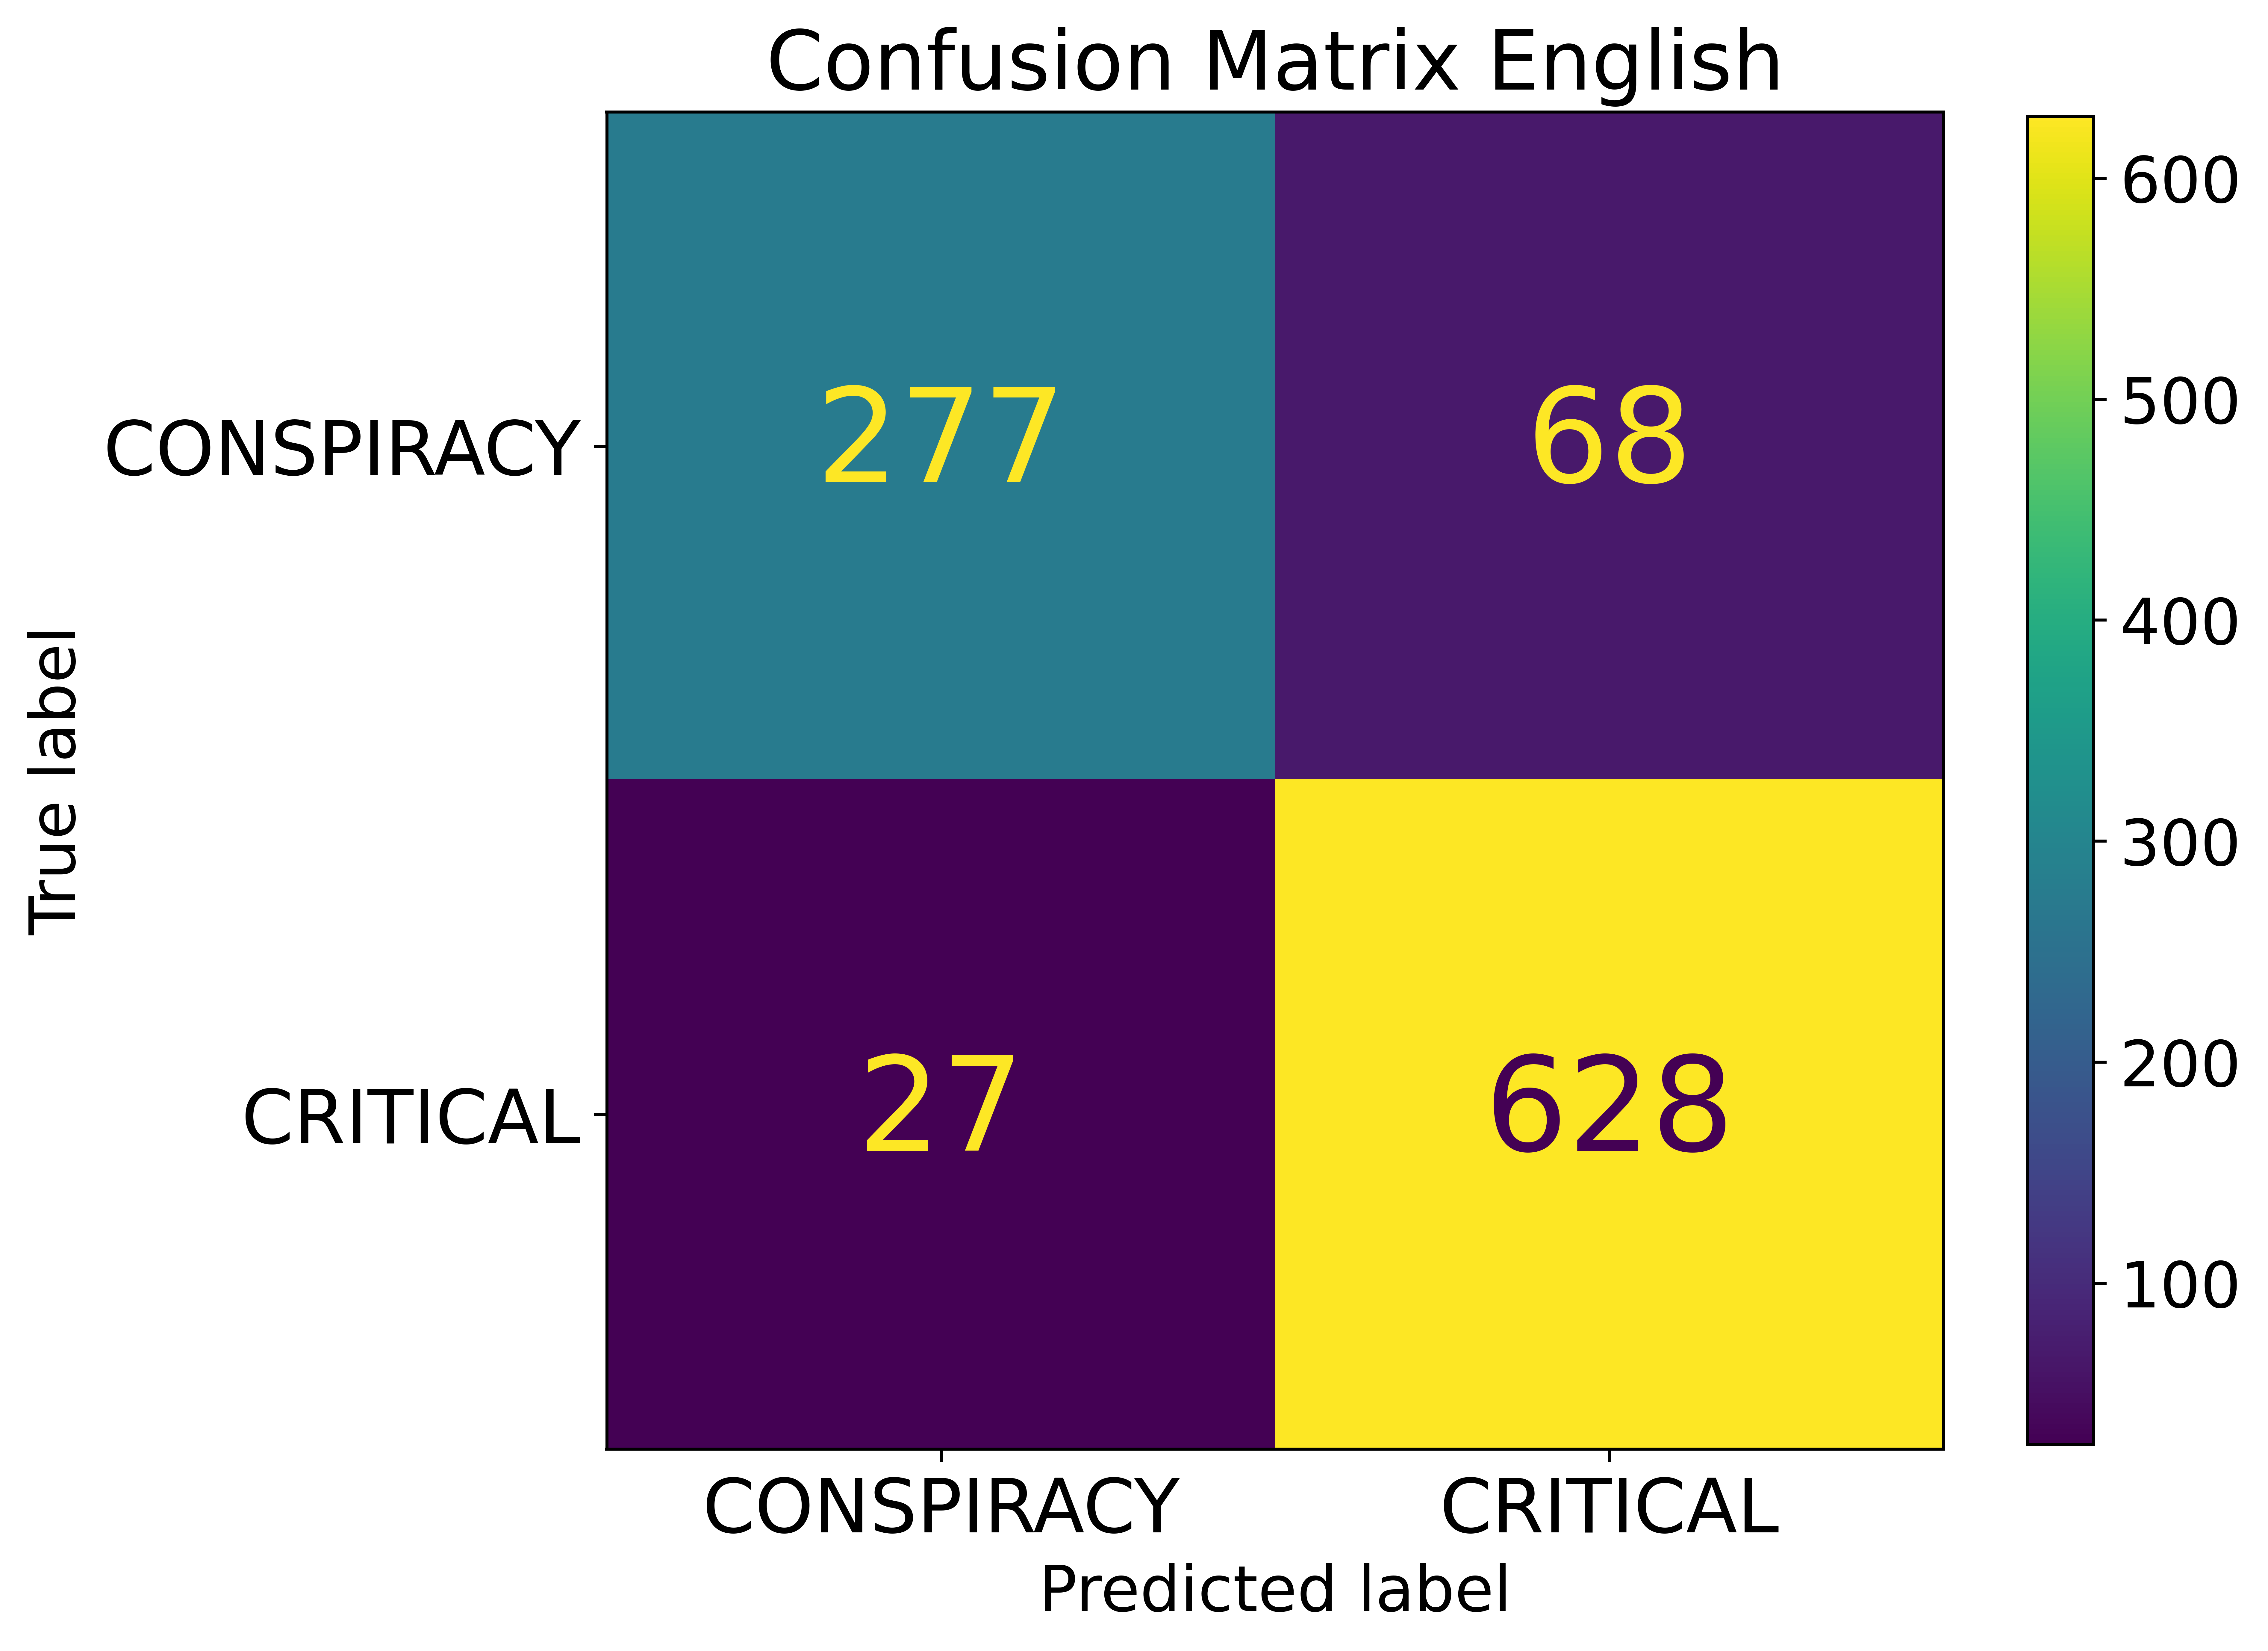
\includegraphics[width=0.49\linewidth]{Images/confusion_matrix_en_v3.png}
    }
    %\hspace{0.05\linewidth} % Adjust the horizontal space between figures
    \subfloat[Confusion matrix for the Spanish dataset\label{fig:confusion_matrix_spanish}]{
        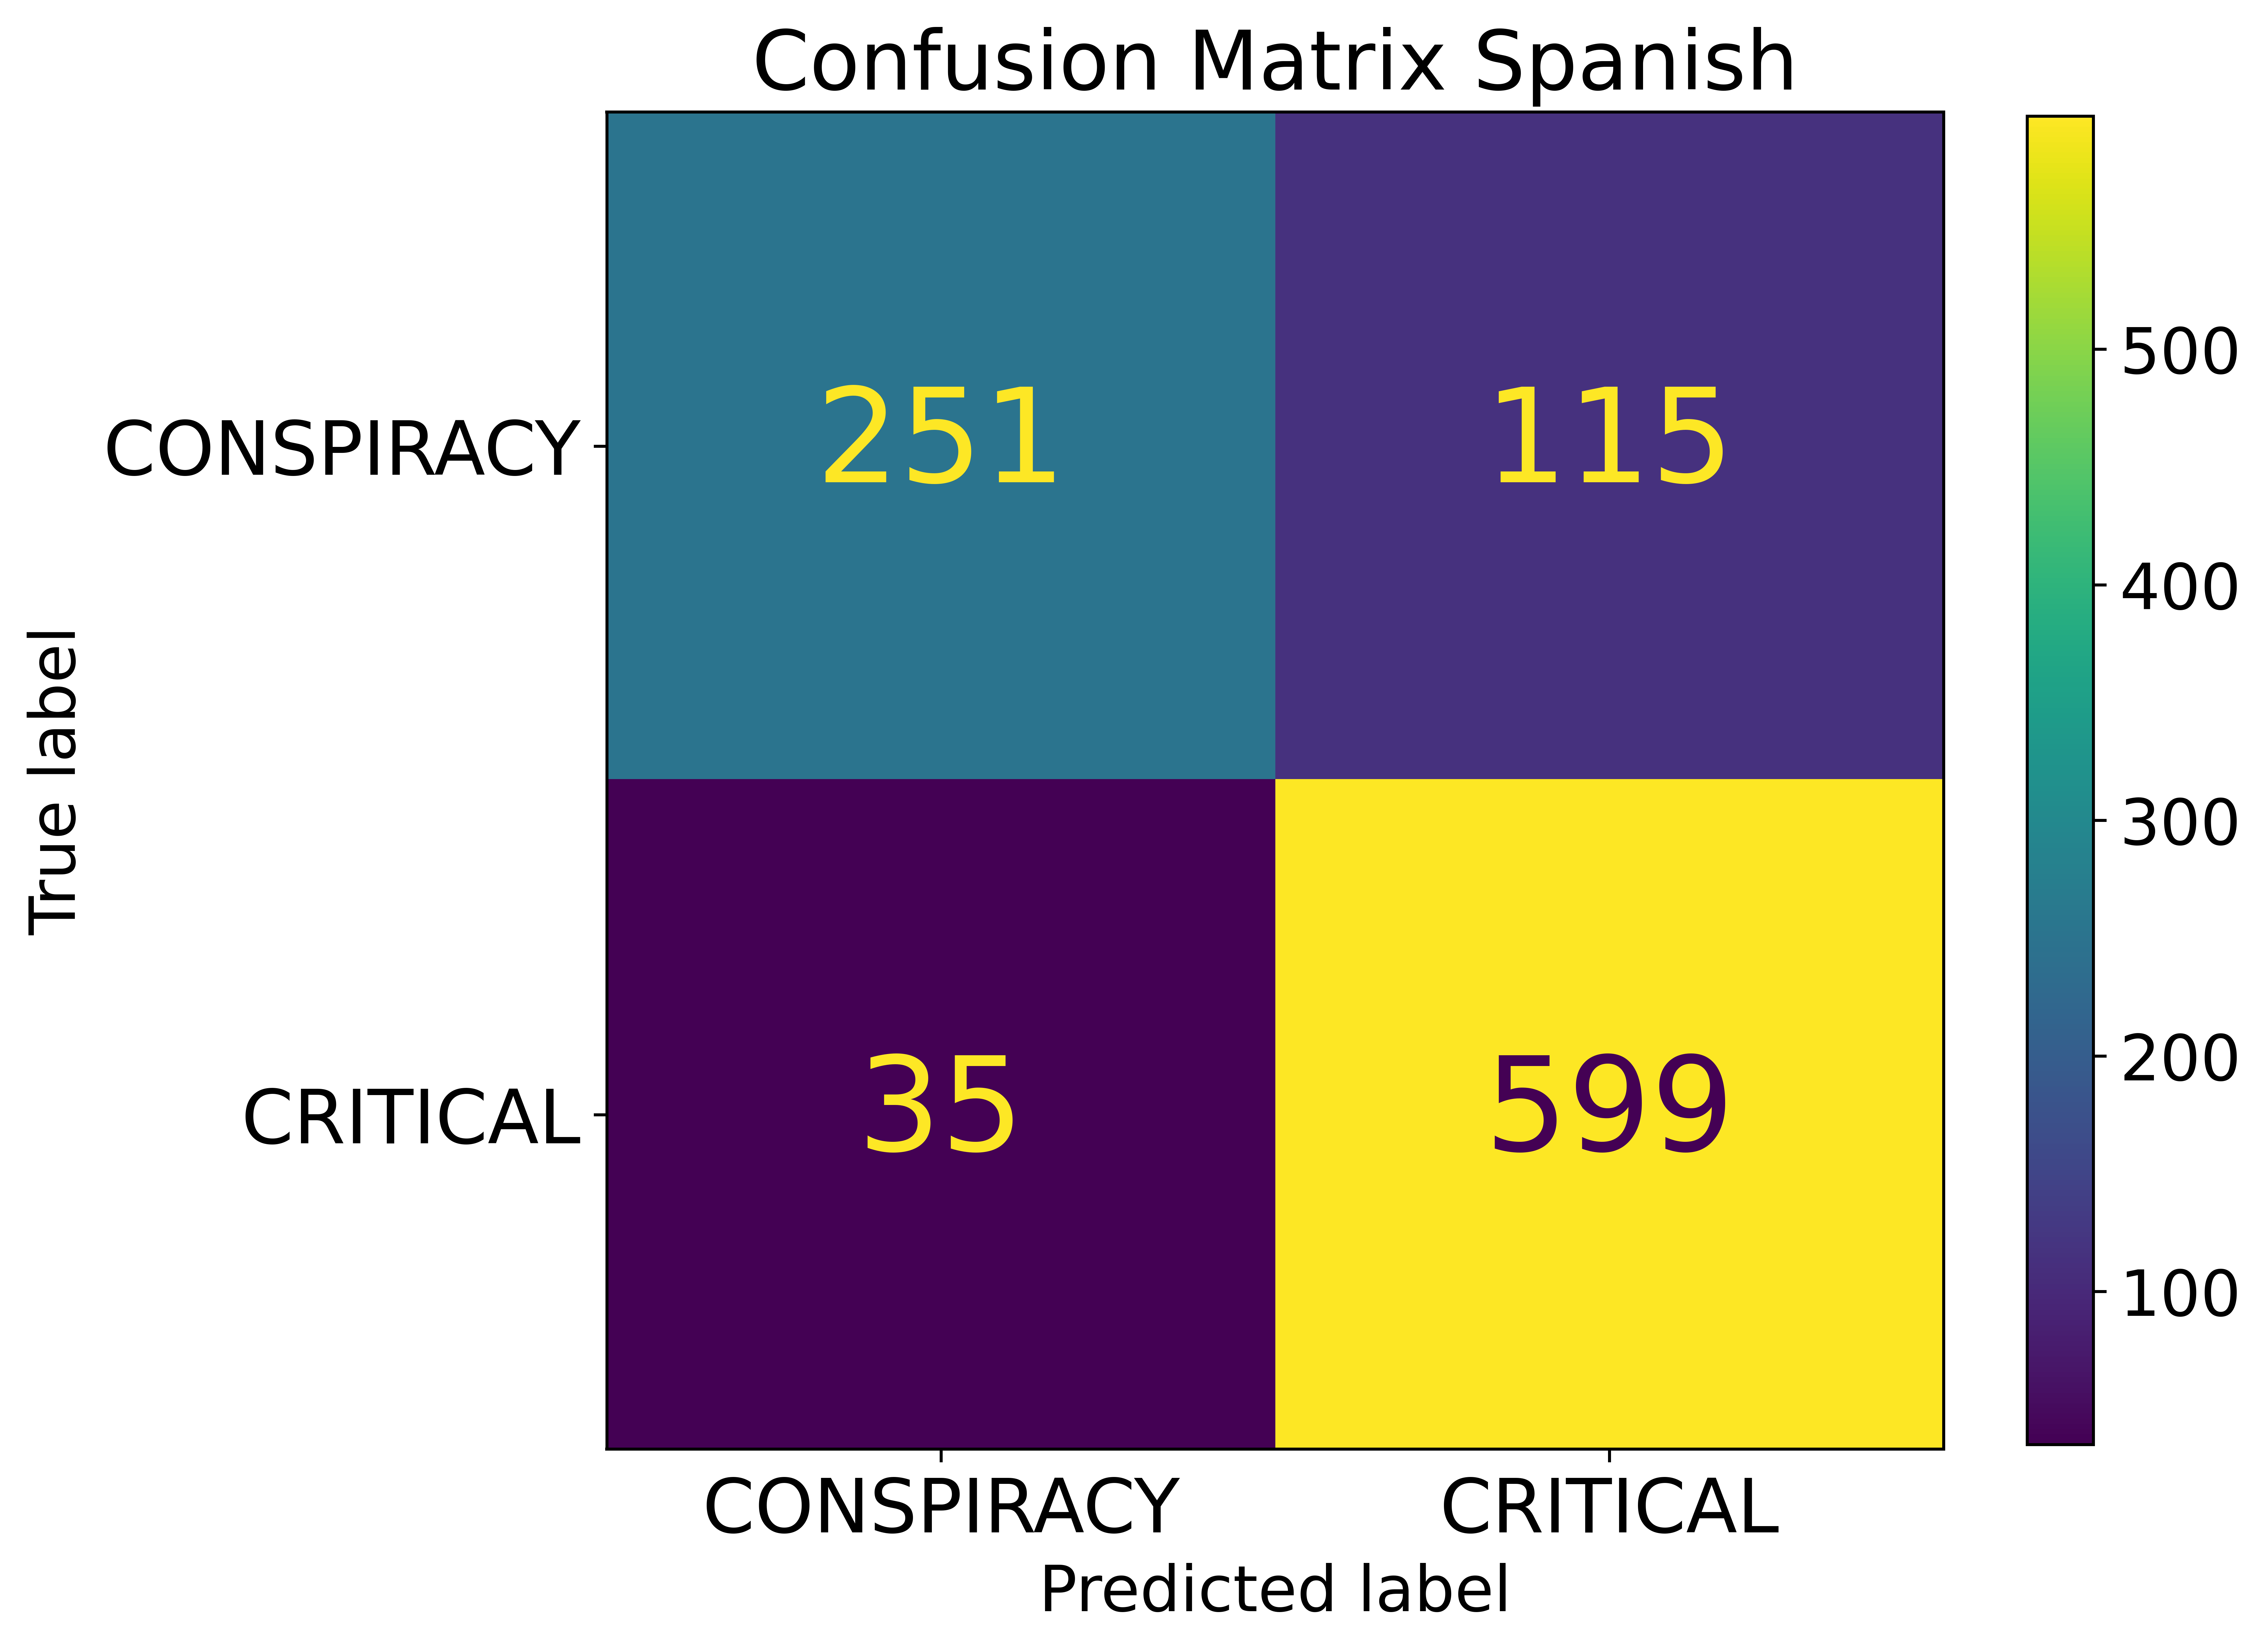
\includegraphics[width=0.49\linewidth]{Images/confusion_matrix_es_v3.png}
    }
    \caption{Confusion matrix of binary classification for the English and the Spanish datasets}
    \label{fig:confusion_matrix_en_es}
\end{figure}
\FloatBarrier

From the confusion matrix, it is evident that in the Spanish dataset, the model frequently misclassifies critical texts as conspiracy. Specifically, out of 634 critical texts, 35 were misclassified as conspiracy, yielding an error rate of approximately 5.52\%. Conversely, of the 366 conspiracy texts, 115 were incorrectly labeled as critical, resulting in a significantly higher error rate of approximately 31.4\%. In the English dataset, the pattern differs slightly. Out of 655 critical texts, 27 were misclassified as conspiracy, resulting in an error rate of approximately 4.12\%. On the other hand, out of 345 conspiracy texts, 68 were incorrectly labeled as critical, leading to an error rate of approximately 19.7\%. This comparative analysis indicates that while the model generally exhibits greater difficulty in accurately classifying conspiracy texts in both datasets, the Spanish dataset demonstrates a particularly high error rate for misclassifying this category.

Text length can significantly influence classification tasks, as longer texts often introduce greater complexity but at the same time can give more context that the model must interpret. The following plots illustrate the distribution of text lengths for the false positives in both the English and Spanish datasets.


\begin{figure}[h]
\centering
\begin{subfigure}
\centering
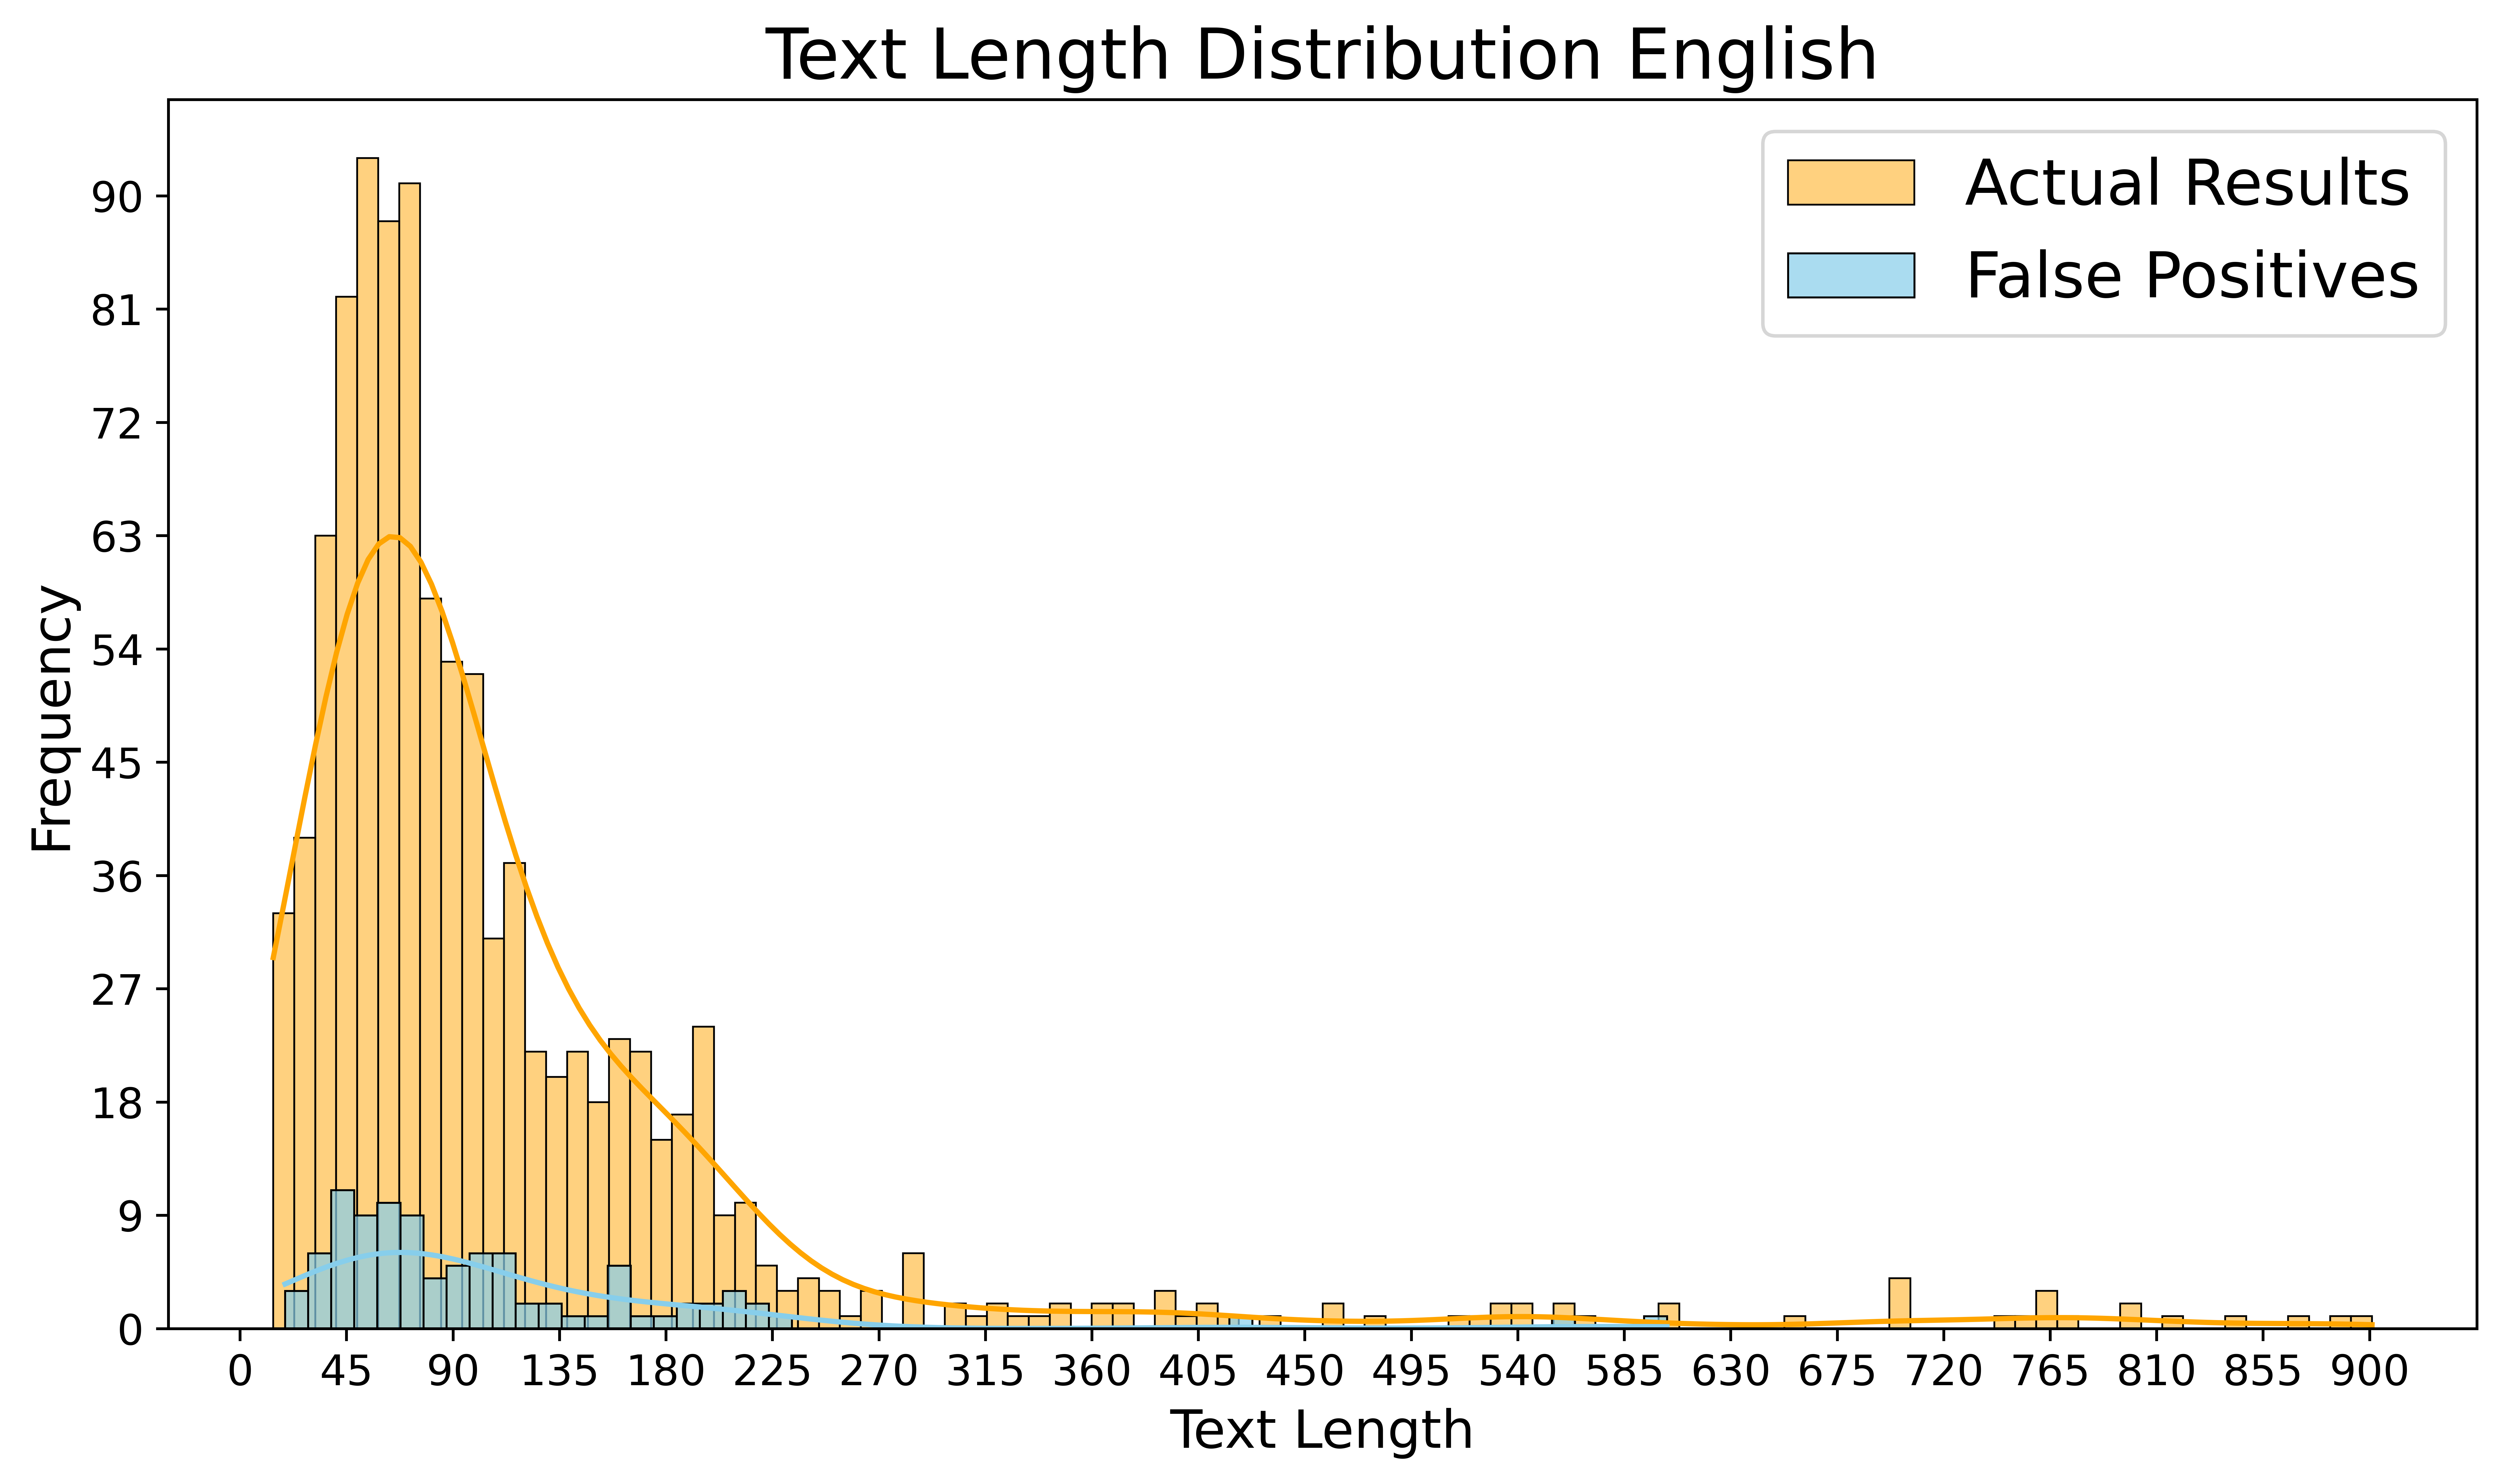
\includegraphics[width=0.86\linewidth, height=0.3\textheight]{Images/text_length_distribution_english_v2.png}
\caption{\small Text length distribution in false positives for the English dataset}
\label{fig:text_length_en}
\end{subfigure}
\begin{subfigure}
\centering
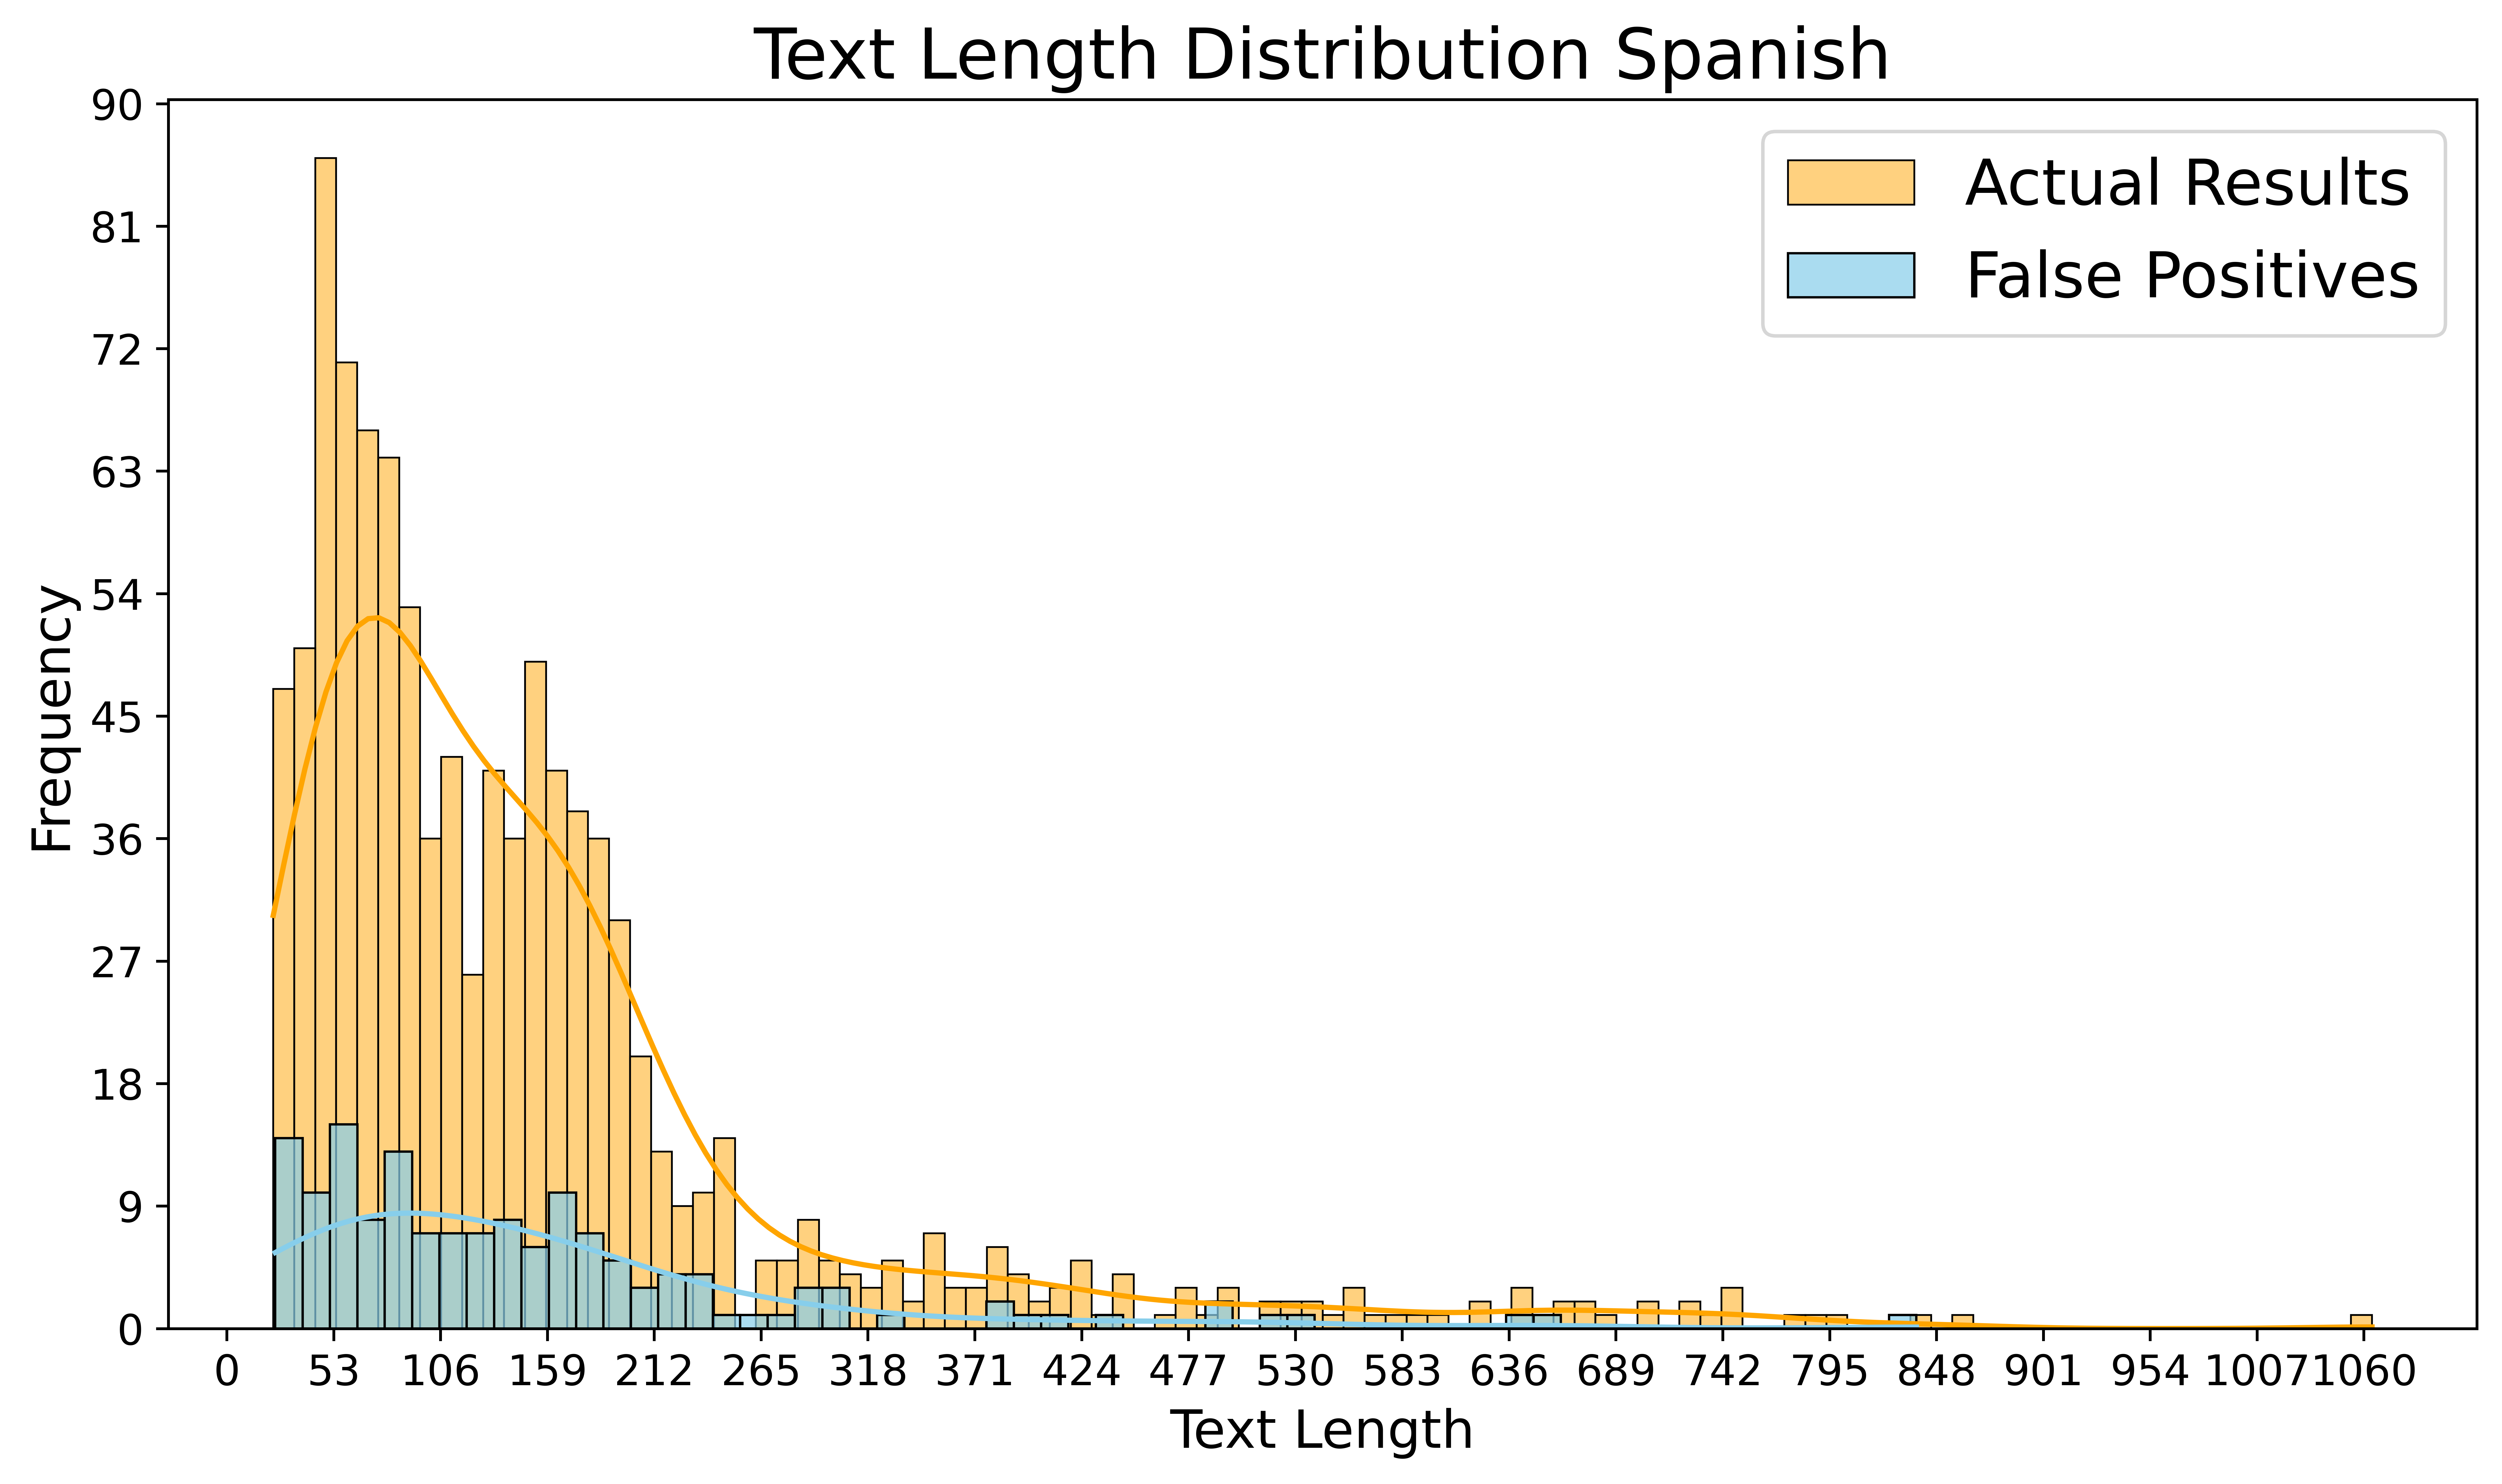
\includegraphics[width=0.86\linewidth, height=0.3\textheight]{Images/text_length_distribution_spanish_v2.png}
\caption{\small Text length distribution in false positives for the Spanish dataset}
\label{fig:text_length_es}
\end{subfigure}
\caption{\small Text length distribution in false positives for the English and Spanish datasets}
\label{fig:text_length_en_es}
\end{figure}
\FloatBarrier

Analyzing the text lengths of the false positives in the English dataset, we observe that the text lengths range from 19 to 603 words. The average length of the texts in this dataset is approximately 107 words. This indicates a moderate variation in the lengths of false positive texts, with some texts being relatively short while others are significantly longer. In the Spanish dataset, the text lengths of the false positives range from 24 to 838 words, with an average length of 155 words. This dataset exhibits a wider range of text lengths compared to the English dataset, and the average length is also higher. This suggests that false positives in the Spanish dataset tend to have longer texts on average. The analysis indicates that as texts become longer and more detailed, the model's ability to correctly classify them increases. The additional context and complexity in longer texts introduce more opportunities for the model to better classify the data. As we can observe from Figure \ref{fig:text_length_en_es} the distribution of the false positives follow the actual results, so we can say that we don't find any unexpected behavior in our system.

The high error rate for conspiracy texts in both datasets might be attributed to several factors. Firstly, ambiguity in language plays a significant role. Many texts contain language that can be interpreted as both critical and conspiratorial, especially when discussing contentious topics such as vaccines or government policies. This overlap makes it challenging for the model to draw clear distinctions.
Secondly, the complexity of the context adds to the difficulty. Longer texts provide more context, but they also introduce more opportunities for nuanced or ambiguous statements that the model struggles to classify accurately. The increased detail can obscure the main sentiment or intent of the text.
The limitations of the training data also contribute to the misclassifications, If the training data does not adequately cover the range of expressions and contexts found in the test data. Since the train dataset is unbalanced to the critical texts, the model struggles to identify conspiracy theories.
Cultural and linguistic nuances further complicate the model's performance. The differences between the English and Spanish datasets might be attributed to cultural and linguistic nuances that influence how critical discussions and conspiracy theories are expressed. These nuances can introduce additional complexity for the model, which needs to be sensitive to the specific contexts and idioms used in each language.

\section{Task 2: Span-Level Detection}
Continuing from the binary classification task, we now turn our attention to the more intricate domain of span-level detection. This analysis concentrates on the diverse categories within span text to identify discrepancies between the model's predictions and the actual annotations, by examining the confusion matrices for both the English and Spanish datasets. These matrices visually represent the model's performance, illustrating the frequency of correct predictions for each category and the frequency of misclassifications.

\begin{figure}[H]
    \centering
    \subfloat[Confusion matrix for the English dataset\label{fig:confusion_matrix_en_T2.png}]{
        \includegraphics[width=0.49\linewidth]{Images/confusion_matrix_en_T2_v3.png}
    }
    %\hspace{0.0008\linewidth} % Adjust the horizontal space between figures
    \subfloat[Confusion matrix for the Spanish dataset\label{fig:confusion_matrix_es_T2.png}]{
        \includegraphics[width=0.49\linewidth]{Images/confusion_matrix_es_T2_v3.png}
    }
    \caption{Confusion matrix of span-text categories for the English and the Spanish datasets}
    \label{fig:confusion_matrix_en_es}
\end{figure}
\FloatBarrier

The confusion matrices reveal several notable patterns. For the English dataset, the model correctly identified 858 spans as \textit{Agent} but also mislabeled 342 spans that have been not annotated. In the \textit{Campaigner} category, the model correctly identified 882 spans but misclassified 325 spans that were not annotated. The \textit{Facilitator} category had 308 correct identifications and 229 misclassifications into \textit{No\_Annotation}. The \textit{Negative\_Effect} category had 782 correct identifications but also saw 269 misclassifications. The \textit{Objective} category had 218 correct identifications but 175 misclassifications, and the \textit{Victim} category had 566 correct identifications with 239 misclassifications.

A significant issue is observed with \textit{No\_Annotation}, where spans that should not have been annotated were misclassified into various categories: 498 as \textit{Agent}, 399 as \textit{Campaigner}, 327 as \textit{Facilitator}, 820 as \textit{Negative\_Effect}, 298 as \textit{Objective}, and 375 as \textit{Victim}. This broad issue suggests difficulty in identifying when no annotation is needed.

For the Spanish dataset, the confusion matrix reveals similar challenges. The model correctly identified 308 spans as \textit{Agent} but misclassified 271 spans as \textit{No\_Annotation}. In the \textit{Campaigner} category, 584 spans were correctly identified, but 316 spans were misclassified. The \textit{Facilitator} category had 248 correct identifications with 211 misclassifications. The \textit{Negative\_Effect} category had 930 correct identifications but 351 misclassifications.The \textit{Objective} category had 50 correct identifications with 65 misclassifications. The \textit{Victim} category had 647 correct identifications but 337 spans were misclassified as \textit{No\_Annotation}.

The Spanish model also frequently misclassified \textit{No\_Annotation} spans: 198 as \textit{Agent}, 259 as \textit{Campaigner}, 213 as \textit{Facilitator}, 658 as \textit{Negative\_Effect}, 79 as \textit{Objective}, and 299 as \textit{Victim}.

Comparing the English and Spanish datasets, both exhibit high misclassification rates in the \textit{No\_Annotation} category, indicating challenges in identifying spans that should not be annotated. This issue likely stems from the complexity and varied contexts in which terms appear.

This discrepancy can be attributed to several factors. Model overconfidence may lead to identifying spans based on patterns learned from the training data. This overconfidence might derive from the model's inability to accurately gauge the certainty of its predictions, leading to an excess of false positives. Annotation inconsistencies could also play a role, as human annotators might miss certain spans, especially in lengthy or complex texts, leading to discrepancies between the predicted and actual spans.

The model's contextual sensitivity might also contribute to this issue, as it may be picking up on contextual cues suggesting the presence of relevant spans, even if they were not explicitly annotated. This could indicate the model's sensitivity to linguistic or contextual markers not consistently labeled in the training data. For example, if certain phrases or contexts are typically associated with a specific category in the training data, the model might overgeneralize these associations to the test data.

%%%%%%%%%%%%%%%%%%%%%%%%%%%%%%%%%%%%%%%%%%%%%%%%%%%%%%%%%%%%%%%%%%%%%%%%%%%%%%%%%%%%%%%%%%%%%%%%%%%%%%%%%%%%%%%%%

\chapter{Experiments with LLMs and Multilingual Transformer Models} \label{chap:experiments_LLMs_multilingual}
In this chapter, we explore further experiments conducted after submitting our runs to the shared task. These additional tests aimed to evaluate the effectiveness of both multilingual transformer models and Large Language Models (LLMs). We began by fine-tuning both model types to tailor their predictions, while for LLMs specifically, we also investigated zero-shot learning \textit{(ZSL)} and few-shot learning \textit{(FSL)} scenarios. The objective was to determine whether these approaches could outperform our submitted runs and yield more robust results across the two datasets. We will start with the first task and then continue with the second one.

\section{Experiments Task 1}
This section addresses \textbf{RQ1}, examining the effectiveness of multilingual models and Large Language Models in distinguishing between conspiratorial and critical thinking narratives. We tested various configurations to enhance performance, including fine-tuning multilingual models on both English and Spanish datasets to leverage cross-linguistic strengths. We further evaluated LLMs using zero-shot and few-shot learning to assess their capacity for robust classification without explicit training, as well as the impact of fine-tuning methods incorporating task-specific prompts for optimized results.

\subsection{Multilingual Transformer Models}
The experiments with multilingual transformer models aimed to leverage the capability of handling both English and Spanish texts within a single model. Unlike the earlier approaches where the datasets were translated for consistency, these models were fine-tuned directly on the original language texts using appropriate spaCy models for language-specific embeddings. This approach allowed us to maintain the linguistic richness of each language while enabling the models to process bilingual datasets effectively.

The results of these experiments are shown in Table \ref{tab:performance_T1_multilingual}. We also evaluated ensemble models that combined predictions from the three single multilingual transformers to enhance performance. These ensembles aimed to leverage each model's strengths for more robust predictions. The submitted runs to the shared task are also included in the table for comparison.

\begin{table}[H]
\centering
\footnotesize
\begin{tabular}{lccccccc}
\hline \textbf{Model} & \textbf{Acc.} & \textbf{MCC} & \textbf{Prec.} & \textbf{Recall} & \textbf{F1-Consp} & \textbf{F1-Crit} & \textbf{F1-Macro} \\
\hline
\multicolumn{8}{c}{\textbf{ENGLISH}} \\
\hline
xlm-roberta-large & \textbf{0.8980} & \textbf{0.7715} & 0.9147 & \textbf{0.7768} & \textbf{0.8401} & \textbf{0.9251} & \textbf{0.8826} \\
bert-base-multilingual & 0.8760 & 0.7237 & \textbf{0.9300} & 0.6928 & 0.7940 & 0.9113 & 0.8527 \\
xlm-roberta-base & 0.8750 & 0.7191 & 0.9015 & 0.7159 & 0.7981 & 0.9095 & 0.8538 \\
ensemble-3\_multilingual & 0.8900 & 0.7555 & 0.9401 & 0.7275 & 0.8203 & 0.9207 & 0.8705 \\
\hline
\textit{submitted\_run} & \textit{0.9050} & \textit{0.7872} & \textit{0.9112} & \textit{0.8029} & \textit{0.8536} & \textit{0.9297} & \textit{0.8917} \\
\hline
\multicolumn{8}{c}{\textbf{SPANISH}} \\
\hline
xlm-roberta-large & \textbf{0.8180} & \textbf{0.6027} & 0.8770 & \textbf{0.5847} & \textbf{0.7016} & \textbf{0.8691} & \textbf{0.7854} \\
bert-base-multilingual & 0.7730 & 0.5011 & 0.8564 & 0.4563 & 0.5954 & 0.8423 & 0.7188 \\
xlm-roberta-base & 0.7970 & 0.5632 & \textbf{0.9137} & 0.4918 & 0.6394 & 0.8587 & 0.7491 \\
ensemble-3\_multilingual & 0.8010 & 0.5687 & 0.8957 & 0.5164 & 0.6551 & 0.8602 & 0.7576 \\
\hline
\textit{submitted\_run} & \textit{0.8500} & \textit{0.6722} & \textit{0.8776} & \textit{0.6858} & \textit{0.7699} & \textit{0.8887} & \textit{0.8293} \\
\hline
\end{tabular}
\caption{Performance metrics of multilingual transformer models for binary classification}
\label{tab:performance_T1_multilingual}
\end{table}
\FloatBarrier

While the multilingual transformer models demonstrated promising results, they generally performed slightly worse compared to the submitted runs. For instance, the best-performing multilingual transformer model, \textit{xlm-roberta-large}\footnote{\url{https://huggingface.co/FacebookAI/xlm-roberta-large}}, achieved an accuracy of 0.8980 and an MCC of 0.7715 on the English dataset, which, while strong, did not surpass the submitted run's accuracy of 0.9050 and MCC of 0.7872. Similarly, for the Spanish dataset, the submitted run achieved a higher accuracy (0.8500) and MCC (0.6722) compared to the top-performing multilingual model (0.8180 accuracy and 0.6027 MCC).

These results highlight that although the multilingual transformer models are capable of handling both languages within a single framework, the initial models submitted offered a slightly better fit for their respective languages. One possible reason could be that we provided the model with both the original dataset and the translated one, resulting in an equal amount of data for both monolingual and multilingual models. Nonetheless, the multilingual approach remains valuable for its efficiency in managing bilingual data and reducing the need for separate models, offering a streamlined alternative for multilingual tasks.

\subsection{Zero Shot Learning}
Taking a further step to the most cutting-edge technologies, this section outlines the methodologies used leveraging Large Language Models, prompt-based generation, and optimized data handling to ensure efficient and scalable performance. These experiments were conducted to evaluate whether LLMs, even though not designed explicitly for binary classification, could achieve better results than specialized fine-tuned transformer based models. Various LLMs were selected for their ability to handle instruction-based tasks effectively.

These models were loaded using half-precision floating-point numbers to reduce memory consumption while maintaining computational efficiency. Additionally, was included an option for 4-bit quantization to further reduce the memory footprint, making it feasible to run these models on more limited hardware resources. The classification system was powered by a text-generation pipeline, built using Hugging Face’s transformer libraries. This pipeline handled the input texts and generated deterministic responses. The output length was capped at 80 tokens to keep the generated responses concise and focused on the classification task. 

At the core of the classification process was a structured prompt in the language of each dataset, guiding the model to categorize texts into one of the two categories. For zero-shot learning, the Spanish dataset was prompted in Spanish, while the English dataset used an English prompt. The prompt used for the English dataset was as follows:

\begin{center}
\begin{flushleft}
\footnotesize
\texttt{
prompt = \textquotedblleft  \textless s\textgreater[INST] \textless\textless SYS\textgreater\textgreater \\
You are an expert critical thinker specialized in analyzing public health narratives, particularly regarding the COVID-19 pandemic.You are tasked with classifying a text into one of these two categories: \\
1. CRITICAL THINKING: Texts that question major public health decisions but do not suggest that secret, powerful, or malevolent groups are behind these decisions. \\
2. CONSPIRACY THEORIES: Texts that imply public health decisions, especially those regarding the COVID-19 pandemic, are part of a plot orchestrated by secret, powerful, and malevolent groups. \\
Now, say if the following text is 'CRITICAL' or 'CONSPIRACY': \\
\textless\textless/SYS\textgreater\textgreater \\
\{user\_text\} \\
\mbox{[/INST]</s>} \textquotedblright \\
}
\end{flushleft}
\end{center}


\begin{table}[h]
    \centering
    %\small
    \begin{tabular}{lccccc}
        \hline
        \textbf{Model} & \textbf{Acc.} & \textbf{MCC} & \textbf{F1-macro} & \textbf{F1-Consp.} & \textbf{F1-Crit.}   \\
        \hline
        \multicolumn{6}{c}{\textbf{ENGLISH}} \\
        \hline
        Llama-3.2-3B-Instruct & 0.5010 & 0.1124 & 0.5010 & 0.5035  & 0.4985  \\
        gemma-2-9b-it & 0.6400 & \textbf{0.4602} & \textbf{0.6394} & \textbf{0.6545} & 0.6245   \\
        Mistral-7B-Instruct & 0.3670 & 0.0921 & 0.2953 & 0.5201 & 0.0705   \\
        gemma-7b-it & \textbf{0.6500} & -0.0246 & 0.3993 & 0.0113 & \textbf{0.7874}  \\
        \hline
        \textit{submitted\_run} & \textit{0.9050} & \textit{0.7872} & \textit{0.8917} & \textit{0.8536} & \textit{0.9297}   \\
        \hline
        \hline
        \multicolumn{6}{c}{\textbf{SPANISH}} \\
        \hline
        Llama-3.2-3B-Instruct & \textbf{0.6470} & 0.1260 & 0.4671 & 0.1575  & \textbf{0.7767}  \\
        gemma-2-9b-it & 0.5600 & \textbf{0.3265} & \textbf{0.5517} & \textbf{0.6127} & 0.4907   \\
        Mistral-7B-Instruct & 0.4800 & 0.0761 & 0.4777 & 0.5122 & 0.4433   \\
        gemma-7b-it & 0.3730 & 0.0099 & 0.2883 & 0.5338 & 0.0427   \\
        \hline
        \textit{submitted\_run} & \textit{0.8500} & \textit{0.6722}  & \textit{0.8293} & \textit{0.7699} & \textit{0.8887}   \\
        \hline
    \end{tabular}
    \caption{Performance metrics of zero-shot learning for binary classification}
    \label{tab:performance_llms_T1_zero_shots}
\end{table}
\FloatBarrier


Analyzing the results in Table \ref{tab:performance_llms_T1_zero_shots}, it becomes evident that the zero-shot learning achieved significantly lower performance compared to the submitted systems. The highest accuracy achieved by the zero-shot LLMs was 0.6500 with \textit{gemma-7b-it}\footnote{\url{https://huggingface.co/google/gemma-7b-it}} model on the English dataset, which is considerably lower than the 0.9050 accuracy of the submitted English system. The highest MCC among the zero-shot models was 0.4602, achieved by \textit{gemma-2-9b-it}\footnote{\url{https://huggingface.co/google/gemma-2-9b-it}} model on the English dataset, which is also substantially lower than the MCC of 0.7872 achieved by the submitted system. This underlines that the zero-shot learning reached very poor performance compared to the submitted systems, indicating that without fine-tuning, LLMs struggle to match the effectiveness of models specifically trained for this task.

The suboptimal performance of zero-shot learning in the binary classification task likely stems from several factors. One key issue is the nuanced difference between Critical and Conspiracy texts, which may be too subtle for an LLM to distinguish without fine-tuning. The distinctions in language used across these categories often involve tone or implied intentions, which LLMs might not capture with generic knowledge and prompts alone. Consequently, the models may have failed to differentiate adequately between texts that question public health decisions and those implying a hidden agenda, leading to misclassifications.

Another reason could be that the LLMs did not fully grasp the classification task despite the structured prompt. The complex, instruction-based prompt may not have been enough to guide the model effectively, as zero-shot learning relies heavily on how well the task aligns with the model’s existing knowledge. Furthermore, without task-specific training, the LLMs were prone to overgeneralization or an inadequate representation of the decision boundaries between the two categories.

\subsection{Few Shot Learning}
We incorporated few-shot learning into our experiments to assess whether including examples in the prompts would enhance the models' classification accuracy compared to the zero-shot approach. 

By providing five examples per category, we aimed to give the models a clearer understanding of how to differentiate between the two categories. This approach aligns with recent research emphasizing the importance of guiding large language models through well-defined prompts to improve performance in text classification tasks \cite{peskine2023definitions}. Also in this case each dataset was prompted in its respective language.

The complete performance results are presented in Table \ref{tab:performance_llms_T1_few_shots_text_gen}, and the prompt in English used for these experiments is detailed below.

\begin{center}
\begin{flushleft}
\footnotesize
\texttt{
prompt = \textquotedblleft  \textless s\textgreater[INST] \textless\textless SYS\textgreater\textgreater \\
You are an expert critical thinker specialized in analyzing public health narratives, particularly regarding the COVID-19 pandemic. You are tasked with classifying a text into one of these two categories: \\
1. CRITICAL THINKING: Texts that question major public health decisions but do not suggest that secret, powerful, or malevolent groups are behind these decisions. \\
2. CONSPIRACY THEORIES: Texts that imply public health decisions, especially those regarding the COVID-19 pandemic, are part of a plot orchestrated by secret, powerful, and malevolent groups. \\
Here below there are some examples: \\
------ Start of the Examples ----- \\
\textless EXAMPLES\textgreater \\
------ End of the Examples ------ \\
Now, say if the following text is 'CRITICAL' or 'CONSPIRACY': \\
\textless\textless/SYS\textgreater\textgreater \\
\{user\_text\} \\
\mbox{[/INST]</s>} \textquotedblright  \\
}
\end{flushleft}
\end{center}


\begin{table}[H]
    \centering
    %\small
    \begin{tabular}{lccccc}
        \hline
        \textbf{Model} & \textbf{Acc.} & \textbf{MCC} & \textbf{F1-macro} & \textbf{F1-Cons.} & \textbf{F1-Crit.}   \\
        \hline
        \multicolumn{6}{c}{\textbf{ENGLISH}} \\
        \hline
        Llama-3.2-3B-Instruct & \textbf{0.6970} & 0.2559 & 0.5635 & 0.3221  & \textbf{0.8049}  \\
        gemma-2-9b-it         & 0.6870 & \textbf{0.5049} & \textbf{0.6869} & \textbf{0.6822} & 0.6916   \\
        Mistral-7B-Instruct   & 0.5090 & 0.2164 & 0.5039 & 0.5540 & 0.4538   \\
        gemma-7b-it           & 0.5410 & 0.1208 & 0.5361 & 0.4883 & 0.5839   \\
        \hline
        \textit{submitted\_run} & \textit{0.9050} & \textit{0.7872} & \textit{0.8917} & \textit{0.8536} & \textit{0.9297}   \\
        \hline
        \hline
        \multicolumn{6}{c}{\textbf{SPANISH}} \\
        \hline
        Llama-3.2-3B-Instruct & \textbf{0.6480} & 0.1315 & 0.4750 & 0.1737  & \textbf{0.7764}  \\
        gemma-2-9b-it         & 0.5910 & \textbf{0.3322} & \textbf{0.5859} & \textbf{0.6181} & 0.5597   \\
        Mistral-7B-Instruct   & 0.6410 & 0.0914 & 0.4337 & 0.0911 & 0.7763   \\
        gemma-7b-it           & 0.6440 & 0.1158 & 0.4744 & 0.1759 & 0.7730   \\
        \hline
        \textit{submitted\_run} & \textit{0.8500} & \textit{0.6722}  & \textit{0.8293} & \textit{0.7699} & \textit{0.8887}   \\
        \hline
    \end{tabular}
    \caption{Performance metrics of few-shot learning for binary classification}
    \label{tab:performance_llms_T1_few_shots_text_gen}
\end{table}
\FloatBarrier

\begin{table}[h]
    \centering
    %\small
    \begin{tabular}{lccccc}
        \hline
        \textbf{Model} & \textbf{Acc.} & \textbf{MCC} & \textbf{F1-macro} & \textbf{F1-Cons.} & \textbf{F1-Crit.}   \\
        \hline
        \multicolumn{6}{c}{\textbf{ENGLISH}} \\
        \hline
        Llama-3.2-3B-Instruct & \textbf{0.6970} & 0.2559 & 0.5635 & 0.3221  & \textbf{0.8049}  \\
        gemma-2-9b-it         & 0.6870 & \textbf{0.5049} & \textbf{0.6869} & \textbf{0.6822} & 0.6916   \\
        Mistral-7B-Instruct   & 0.5090 & 0.2164 & 0.5039 & 0.5540 & 0.4538   \\
        gemma-7b-it           & 0.5410 & 0.1208 & 0.5361 & 0.4883 & 0.5839   \\
        \hline
        \textit{submitted\_run} & \textit{0.9050} & \textit{0.7872} & \textit{0.8917} & \textit{0.8536} & \textit{0.9297}   \\
        \hline
        \hline
        \multicolumn{6}{c}{\textbf{SPANISH}} \\
        \hline
        Llama-3.2-3B-Instruct & \textbf{0.6480} & 0.1315 & 0.4750 & 0.1737  & \textbf{0.7764}  \\
        gemma-2-9b-it         & 0.5910 & \textbf{0.3322} & \textbf{0.5859} & \textbf{0.6181} & 0.5597   \\
        Mistral-7B-Instruct   & 0.6410 & 0.0914 & 0.4337 & 0.0911 & 0.7763   \\
        gemma-7b-it           & 0.6440 & 0.1158 & 0.4744 & 0.1759 & 0.7730   \\
        \hline
        \textit{submitted\_run} & \textit{0.8500} & \textit{0.6722}  & \textit{0.8293} & \textit{0.7699} & \textit{0.8887}   \\
        \hline
    \end{tabular}
    \caption{Performance metrics of few-shot learning for binary classification}
    \label{tab:performance_llms_T1_few_shots_text_gen}
\end{table}
\FloatBarrier


Despite including few-shot examples, the performance improvements were marginal and still significantly lower than the submitted systems. For example, the \textit{gemma-2-9b-it} model on the English dataset achieved an accuracy of 0.6870 and an MCC of 0.5049, which is still substantially lower than the submitted system's accuracy of 0.9050 and MCC of 0.7872. This further emphasizes that even with few-shot learning, the LLMs reached very poor performance compared to the submitted systems. 

\subsection{Zero and Few Shot Learning with the Text Classification Pipeline}
We also explored using the LLM models in \textit{"text-classification"} mode instead of \textit{"text-generation"} as previously employed. This classification pipeline adapted LLMs to return one of the two predefined categories directly from the input text. By streamlining the process, the system avoided generating extra tokens or context, ensuring faster execution and consistent binary labeling. Each dataset entry was processed and classified efficiently, with results recorded alongside the corresponding text and identifier. Unlike the text-generation approach, this method focused solely on categorizing input text rather than generating new content. The performance metrics for zero-shot and few-shot learning in this setup are presented in Table \ref{tab:performance_llms_T1_few_shots_text_classification}.

\begin{table}[h]
    \centering
    \small
    \begin{tabular}{lccccc}
        \hline
        \textbf{Model} & \textbf{Acc.} & \textbf{MCC} & \textbf{F1-macro} & \textbf{F1-Consp.} & \textbf{F1-Crit.}   \\
        \hline
        \multicolumn{6}{c}{\textbf{ZERO SHOT}} \\
        \hline
        \multicolumn{6}{c}{\textbf{English}} \\
        \hline
        Llama-3.2-3B-Instruct & 0.4130 & \textbf{0.0866} & 0.3846 & \textbf{0.5169}  & 0.2522  \\   
        gemma-2-9b-it         & 0.4060 & 0.0683 & 0.3764 & 0.5123 & 0.2404   \\   
        Mistral-7B-Instruct   & \textbf{0.6570} & 0.0526 & \textbf{0.4074} & 0.0228 & \textbf{0.7920}  \\   
        gemma-7b-it           & 0.6500 & -0.0246 & 0.3993 & 0.0113 & 0.7874  \\   
        \hline
        \multicolumn{6}{c}{\textbf{Spanish}} \\
        \hline
        Llama-3.2-3B-Instruct & 0.3920 & \textbf{0.0464} & 0.3283 & \textbf{0.5352}  & 0.1214  \\
        gemma-2-9b-it         & 0.3740 & -0.2007 & 0.3739 & 0.3651 & 0.3826   \\   
        Mistral-7B-Instruct   & \textbf{0.6563} & 0.0000 & \textbf{0.3962} & 0.0000 & \textbf{0.7924}   \\   
        gemma-7b-it           & 0.3730 & 0.0099 & 0.2883 & 0.5338 & 0.0427   \\  
        \hline
        \hline
        \multicolumn{6}{c}{\textbf{FEW SHOT}} \\
        \hline
        \multicolumn{6}{c}{\textbf{English}} \\
        \hline
        Llama-3.2-3B-Instruct & 0.5260 & \textbf{-0.0127} & \textbf{0.4922} & 0.3612  & 0.6232  \\   
        gemma-2-9b-it         & 0.6320 & -0.0813 & 0.3973 & 0.0213 & 0.7734   \\        
        Mistral-7B-Instruct   & 0.3590 & -0.0296 & 0.3057 & \textbf{0.4980} & 0.1134   \\       
        gemma-7b-it           & \textbf{0.6540} & -0.0230 & 0.3954 & 0.0001 & \textbf{0.7908} \\
        \hline
        \multicolumn{6}{c}{\textbf{Spanish}} \\
        \hline
        Llama-3.2-3B-Instruct & 0.4920 & \textbf{-0.0481} & \textbf{0.4730} & 0.3728  & 0.5731  \\   
        gemma-2-9b-it         & \textbf{0.4940} & -0.0624 & 0.4678 & 0.3496 & \textbf{0.5859}   \\       
        Mistral-7B-Instruct   & 0.4250 & -0.1420 & 0.4181 & 0.3547 & 0.4815   \\  
        gemma-7b-it           & 0.3650 & -0.0557 & 0.2847 & \textbf{0.5243} & 0.0451   \\
        \hline
        \hline
        \textit{submitted\_run English} & \textit{0.9050} & \textit{0.7872} & \textit{0.8917} & \textit{0.8536} & \textit{0.9297}   \\
        \textit{submitted\_run Spanish} & \textit{0.8500} & \textit{0.6722}  & \textit{0.8293} & \textit{0.7699} & \textit{0.8887}   \\
        \hline
    \end{tabular}
    \caption{\small Zero and few shot learning in text-classification mode for binary classification}
    \label{tab:performance_llms_T1_few_shots_text_classification}
\end{table}
\FloatBarrier

The results show that the submitted systems, fine-tuned for the binary classification task, also in this case, outperformed the general-purpose LLMs. Their higher accuracy and MCC values emphasize the value of task-specific fine-tuning for better accuracy and reliability. These results indicate that while LLMs can handle binary classification tasks, specialized transformers fine-tuned on task-specific data are more effective. The poor performance of zero-shot and few-shot LLMs compared to the submitted systems underscores the need for fine-tuning in complex classification tasks.

\subsection{Fine-Tuning LLMs}
Recognizing the potentials of LLMs, we fine-tuned them on the task-specific train data, in order to see if the results were better than the approaches with transformers models and the zero and few shot learning methods. 

Fine-tuning Large Language Models involved adapting text-generation models to new tasks, allowing them to specialize in distinguishing between the two categories, using techniques like quantization and Parameter-Efficient Fine-Tuning (PEFT) to optimize performance while managing computational resources.

Quantization was employed to reduce the model's memory footprint by storing weights in a 4-bit format using NormalFloat4 (NF4) precision, complemented by BF16 for computations. This technique allowed the model to retain its processing capabilities while significantly reducing memory usage. To further enhance efficiency, Low-Rank Adaptation (LoRA) \cite{hulora} was used as a PEFT method. LoRA fine-tuned only a small subset of the model’s parameters, specifically those involved in attention projections, while keeping most of the pre-trained weights frozen. 

This approach enabled the model to adapt to the new classification task without the need for extensive parameter updates, thus minimizing computational demands.
Training was configured with small batch sizes, augmented through gradient accumulation, and optimized using an 8-bit compatible optimizer, ensuring effective learning despite the model's size.

\begin{table}[h] 
\centering
\small
\begin{tabular}{lccccc}
\hline 
\textbf{Model} & \textbf{Acc.} & \textbf{MCC} & \textbf{F1-Cons} & \textbf{F1-Crit} & \textbf{F1-macro} \\ 
\hline 
\multicolumn{6}{c}{\textbf{ENGLISH}} \\
\hline 
LLAMA 3.2-3B\_NoAug & 0.9140 & 0.8077 & 0.8677 & 0.9363 & 0.9020 \\
LLAMA 3.2-3B\_DataAug & 0.9110 & 0.8009 & 0.8624 & 0.9342 & 0.8983 \\
LLAMA 3.2-3B-Instruct & 0.8930 & 0.7632 & 0.8243 & 0.9231 & 0.8737 \\ 
%LLAMA 3.2-3B\_ft-es\_transl & 0.8910 & 0.7873 & 0.8604 & 0.9106 & 0.8855 \\
gemma-2-9b-it & 0.9170 & 0.8144 & 0.8744 & 0.9380 & 0.9062 \\ 
LLAMA 3.1-8B & 0.9050 & 0.8037 & 0.8728 & 0.9242 & 0.8985 \\ 
ensemble\_3\_LLMs & 0.9210 & 0.8236 & 0.8819 & 0.9406 & 0.9113 \\
ensemble\_4\_LLMs & \textbf{0.9300} & \textbf{0.8477} & \textbf{0.9011} & \textbf{0.9458} & \textbf{0.9235} \\ 
\hline
\textit{submitted\_run} & \textit{0.9050} & \textit{0.7872} & \textit{0.8536} & \textit{0.9297} & \textit{0.8917}  \\
\hline
\multicolumn{6}{c}{\textbf{SPANISH}} \\
\hline 
LLAMA 3.2-3B\_NoAug & 0.8020 & 0.5770 & 0.7346 & 0.8421 & 0.7883 \\
LLAMA 3.2-3B\_DataAug & 0.8260 & 0.6234 & 0.7119 & 0.8754 & 0.7936 \\
LLAMA 3.2-3B-Instruct & 0.8290 & 0.6268 & 0.7255 & 0.8758 & 0.8007 \\ 
%LLAMA 3.2-3B\_ft-es\_transl & 0.8830 & 0.7465 & \textbf{0.8377} & 0.9085 & 0.8731 \\ 
gemma-2-9b-it & 0.8510 & 0.6737 & 0.7759 & 0.8884 & 0.8322 \\ 
LLAMA 3.1-8B & 0.8620 & 0.7003 & 0.8073 & 0.8925 & 0.8499 \\ 
ensemble\_3\_LLMs & 0.8540 & 0.6810 & 0.7774 & 0.8914 & 0.8344 \\ 
ensemble\_4\_LLMs & \textbf{0.8870} & \textbf{0.7538} & 0.8355 & \textbf{0.9139} & \textbf{0.8747} \\ 
\hline
\textit{submitted\_run} & \textit{0.8500} & \textit{0.6722} & \textit{0.7699} & \textit{0.8887} & \textit{0.8293}  \\
\hline 
\end{tabular} 
\caption{Performance metrics of fine-tuning LLMs for binary classification} 
\label{tab:performance_T1_LLM_fine_tuned} 
\end{table}
\FloatBarrier

\begin{table}[H] 
\centering
\small
\begin{tabular}{lcccc}
\hline 
\multicolumn{5}{c}{BEST PERFORMING TEAMS} \\
\hline 
\textbf{Team} & \textbf{MCC} & \textbf{F1-Cons} & \textbf{F1-Crit} & \textbf{F1-macro} \\ 
\hline 
\multicolumn{5}{c}{\textbf{ENGLISH}} \\
\hline 
\textit{IUCL} & \textit{0.8388} & \textit{0.8947} & \textit{0.9441} & \textit{0.9194} \\
\hline
\multicolumn{5}{c}{\textbf{SPANISH}} \\
\hline 
\textit{SINAI} & \textit{0.7429} & \textit{0.8319} & \textit{0.9091} & \textit{0.8705} \\ 
\hline
\end{tabular} 
\caption{BEST Performance metrics of fine-tuning LLMs for binary classification} 
\label{tab:performance_T1_LLM_fine_tuned} 
\end{table}
\FloatBarrier


\begin{table}[H] 
\centering
\small
\begin{tabular}{lcccc}
\hline 
\multicolumn{5}{c}{BEST PERFORMING TEAMS} \\
\hline 
\textbf{Team} & \textbf{MCC} & \textbf{F1-Cons} & \textbf{F1-Crit} & \textbf{F1-macro} \\ 
\hline 
\multicolumn{5}{c}{\textbf{ENGLISH}} \\
\hline 
\textit{IUCL} & \textit{0.8388} & \textit{0.8947} & \textit{0.9441} & \textit{0.9194} \\
\hline
\multicolumn{5}{c}{\textbf{SPANISH}} \\
\hline 
\textit{SINAI} & \textit{0.7429} & \textit{0.8319} & \textit{0.9091} & \textit{0.8705} \\ 
\hline
\end{tabular} 
\caption{BEST Performance metrics of fine-tuning LLMs for binary classification} 
\label{tab:performance_T1_LLM_fine_tuned} 
\end{table}
\FloatBarrier


Despite not using the full computational power of the LLMs, this approach resulted in significant performance gains. As presented in Table \ref{tab:performance_T1_LLM_fine_tuned}, fine-tuned models such as \textit{gemma-2-9b-it} model for the English dataset achieved an accuracy of 0.9170 and an MCC of 0.8144, surpassing the metrics of the submitted English run. The ensemble models \textit{(Llama 3.2-3B-Instruct, gemma-2-9b-it, Llama 3.1-8B and Llama-3.2-3B)} achieved even higher results, with an accuracy of 0.9300 and an MCC of 0.8477. In the case of the Spanish dataset, fine-tuning led to similar improvements, with the best model reaching an accuracy of 0.8870 and an MCC of 0.7538. While these results outperformed the submitted Spanish run's metrics (0.8500 accuracy and 0.6722 MCC), they demonstrated the benefits of adapting LLMs through fine-tuning.

Moreover, fine-tuning an LLM, even with optimizations like quantization that limit the model's full power, not only outperformed out submitted systems but also achieved the best results in the official ranking of the shared task. The complete official ranking of the shared task can be found in Appendix \ref{chap:appendix_B} \cite{korencic2024oppositional}. This indicates that the specialized adaptation of LLMs through fine-tuning remains a powerful approach, providing state-of-the-art performance in binary classification tasks.

\subsection{Fine-Tuning LLMs with Zero and Few Shot Learning}
In this section, we extended traditional fine-tuning of LLMs by incorporating a structured prompt into the training process. Our goal was to determine whether adding a task-specific prompt could enhance the model's performance or help it converge more quickly to the results achieved with standard fine-tuning. To maintain consistency and gain meaningful insights, we used the \textit{Llama-3.2-3B-Instruct}\footnote{\url{https://huggingface.co/meta-llama/Llama-3.2-3B-Instruct}} model across all experiments, testing two distinct approaches.

The first approach involved using a task-specific prompt integrated directly into the input data during preprocessing. This prompt described the classification task clearly, ensuring that each text input was prefixed with detailed instructions for the model. The prompt was tokenized together with the input texts.

The second approach added a twist by dynamically integrating the task-specific context directly during model execution. Instead of embedding the prompt during preprocessing, we employed a custom \textit{PromptContextTrainer} class to concatenate the prompt with each input batch at runtime. This meant that the model always received the instruction in real-time, ensuring a consistent understanding of the task context. We modified the loss computation to include this added context, keeping the model well-informed of the classification goals.

The prompt used for the zero shot learning in English was the following:
\begin{center}
\begin{flushleft}
\footnotesize
\texttt{
prompt = \textquotedblleft \mbox{<s>[INST]}
You are tasked with classifying whether a given text is a CRITICAL statement questioning public health decisions, or a CONSPIRACY narrative alleging a secret plot related to the pandemic.
\mbox{[/INST]</s>} \textquotedblright \\
}
\end{flushleft}
\end{center}

The performance metrics summarized in Table \ref{tab:performance_fi_with_ZSL_T1} show that traditional fine-tuning without prompts, labeled \textit{No\_ZSL}, was still the best method. This demonstrates that a straightforward approach effectively utilized the models' pre-trained knowledge for binary classification. However, incorporating structured prompts had mixed effects. The first method, which embedded prompts during preprocessing (\textit{ZSL\_preproc}), led to a decline in performance, with the English model's accuracy dropping to 0.9050 and an even more substantial decrease for the Spanish model. This suggests that integrating prompts at the preprocessing stage may have disrupted the models' understanding and introduced unnecessary complexity. In contrast, the second method, which dynamically integrated prompts during training (\textit{ZSL\_train\_ctx}), produced results closer to the baseline, with only minor differences in accuracy and MCC. Still, even this approach did not surpass the performance of traditional fine-tuning, indicating that the added task-specific prompts offered limited benefits.


\begin{table}[H]
\centering
\small
\begin{tabular}{lccccc}
\hline
\textbf{Model} & \textbf{Acc.} & \textbf{MCC} & \textbf{F1-Cons} & \textbf{F1-Crit} & \textbf{F1-Macro}\\
\hline
\multicolumn{6}{c}{\textbf{ENGLISH}} \\
\hline
Llama-3.2-3B\_No\_ZSL & \textbf{0.9110} & \textbf{0.8009} & \textbf{0.8624} & \textbf{0.9342} & \textbf{0.8983}   \\
Llama-3.2-3B\_ZSL\_preproc & 0.9050 & 0.7883 & 0.8494 & 0.9306 & 0.8900  \\
Llama-3.2-3B\_ZSL\_train\_ctx & 0.9100 & 0.7987 & 0.8649 & 0.9325 & 0.8987  \\
\hline
\multicolumn{6}{c}{\textbf{SPANISH}} \\
\hline
Llama-3.2-3B\_No\_ZSL & \textbf{0.8830} & \textbf{0.7465} & \textbf{0.8377} & \textbf{0.9085} & \textbf{0.8731}   \\
Llama-3.2-3B\_ZSL\_preproc & 0.8520 & 0.6760 & 0.7849 & 0.8872 & 0.8360  \\
Llama-3.2-3B\_ZSL\_train\_ctx & 0.8710 & 0.7196 & 0.8190 & 0.8998 & 0.8594  \\
\hline
\end{tabular}
\caption{Performance metrics for fine-tuned models with ZSL for binary classification}
\label{tab:performance_fi_with_ZSL_T1}
\end{table}
\FloatBarrier

Given that the zero-shot learning approach did not produce performance improvements, we explored a few-shot learning strategy to see if adding explicit examples to the prompts would yield better results. In this setup, we included five sample texts for critical and conspiracy categories, aiming to give the model a clearer understanding of the classification task. The prompt used is shown below:
\begin{center}
\begin{flushleft}
\footnotesize
\texttt{
prompt = \textquotedblleft \mbox{<s>[INST]}
You are tasked with classifying whether a given text is a CRITICAL statement questioning public health decisions, or a CONSPIRACY narrative alleging a secret plot related to the pandemic.\\
Here below there are some examples: \\
------ Start of the Examples ----- \\
-- Start Examples of CRITICAL texts --  \\
<EXAMPLES\_CRITICAL> \\
-- End Examples of CRITICAL texts --  \\
-- Start Examples of CONSPIRACY texts -- \\
<EXAMPLES\_CONSPIRACY> \\
-- End Examples of CONSPIRACY texts -- \\
------ End of the Examples ------ \\
\mbox{[/INST]</s>} \textquotedblright \\
}
\end{flushleft}
\end{center}
As shown in Table \ref{tab:performance_ft_with_ZSL_FSL}, the few-shot learning results fell short compared to the baseline models fine-tuned without prompts. In the first approach, where examples were incorporated into the prompt during preprocessing, performance declined. The English model's accuracy dropped to 0.8840, with an MCC of 0.7401, while the Spanish model's accuracy decreased to 0.8330, with an MCC of 0.6291. This marked a clear regression from the strong performance of traditional fine-tuning, suggesting that embedding examples during preprocessing introduced unnecessary complexity instead of enhancing clarity.

The second approach, which dynamically added examples during training, produced slightly better results but still failed to match the baseline. The English model achieved 89.10\% accuracy with an MCC of 0.7552, and the Spanish model showed modest improvement but continued to lag behind the original fine-tuned models. Even with more refined integration, the examples did not elevate the performance beyond that of straightforward fine-tuning.

Overall, the few-shot learning strategy, despite incorporating explicit examples, did not improve the model performance. The baseline models using standard fine-tuning without prompts remained superior. These findings indicate that the added complexity of few-shot prompts may have caused confusion rather than delivering the intended benefits.


\begin{table}[H]
    \centering
    %\renewcommand{\arraystretch}{1.4}
    \small
    \begin{tabular}{lccccc}
        \hline
        \textbf{Model} & \textbf{Acc.} & \textbf{MCC} & \textbf{F1-Cons} & \textbf{F1-Crit} & \textbf{F1-Macro}\\
        \hline
        \multicolumn{6}{c}{\textbf{ENGLISH}} \\
        \hline
        Llama-3.2-3B\_No\_FSL & \textbf{0.9110} & \textbf{0.8009} & \textbf{0.8624} & \textbf{0.9342} & \textbf{0.8983} \\
        Llama-3.2-3B\_FSL\_preproc & 0.8840 & 0.7401 & 0.8135 & 0.9158 & 0.8647  \\
        Llama-3.2-3B\_FSL\_train\_ctx & 0.8910 & 0.7552 & 0.8305 & 0.9197 & 0.8751 \\ 
        \hline 
        \multicolumn{6}{c}{\textbf{SPANISH}} \\
        \hline
        Llama-3.2-3B\_No\_FSL & \textbf{0.8830} & \textbf{0.7465} & \textbf{0.8377} & \textbf{0.9085} & \textbf{0.8731} \\ 
        Llama-3.2-3B\_FSL\_preproc & 0.8330 & 0.6291 & 0.6888 & 0.7756 & 0.8581  \\ 
        Llama-3.2-3B\_FSL\_train\_ctx & 0.8520 & 0.6761 & 0.7846 & 0.8870 & 0.8698  \\ 
        \hline 
    \end{tabular}
    \caption{Performance metrics for fine-tuned models with FSL for binary classification}
    \label{tab:performance_ft_with_ZSL_FSL}
\end{table}
\FloatBarrier

%%%%%%%%%%%%%%%%%%%%%%%%%%%%%%%%%%%%%%%%%%%%%%%%%%%%%%%%%%%%%%%%%%%%%%%%%%%%%%%%%%%%%%%%%%%%%%%%
%%%%%%%%%%%%%%%%%%%%%%%%%%%%%%%%%%%%%%%%%%%%%%%%%%%%%%%%%%%%%%%%%%%%%%%%%%%%%%%%%%%%%%%%%%%%%%%%

\section{Experiments Task 2}
Shifting to the second task, this section tackles \textbf{RQ2} by detailing experiments centered on two main strategies: employing multilingual transformer models and exploring zero-shot and few-shot learning with Large Language Models.

Subsection \ref{subsec:multilingual_models_T2} describes our use of fine-tuned multilingual transformer models to handle both English and Spanish datasets seamlessly, leveraging the linguistic capabilities of spaCy to retain nuanced language features, while Subsection \ref{subsec:ZSL_FSL_LLMs_T2} examines the application of zero-shot and few-shot learning with LLMs, highlighting the impact of prompt designs and the inclusion of example texts on model performance.

\subsection{Multilingual Transformer Models} \label{subsec:multilingual_models_T2}
Also for the further experiments on the second task, we made use of fine-tuning multilingual transformer models. This method changes from the one described in Section \ref{sec:system_T2}, by enabling multilingual processing to allow a single model to handle datasets in both English and Spanish. This approach leverages multilingual transformer models that can be fine-tuned on both English and Spanish datasets simultaneously, streamlining the training process and enabling seamless predictions across languages. 

In addition, there was not necessary to augment the dataset via synonym replacement because we could use the two datasets available together. Indeed, a key aspect of this method is the use of language-specific spaCy models during preprocessing. This ensures that the linguistic features and nuances of each language are accurately captured during tokenization and text processing. The appropriate spaCy model is dynamically selected based on the language of each text. During training, the model learns to identify and classify entities across languages using the BIO tagging scheme. This bilingual capability means that after training, the same model can make predictions on both English and Spanish datasets without needing any modifications or separate models. This ensures consistency in entity recognition across different languages, making it especially useful for multilingual applications. 

In Table \ref{tab:performance_T2_multilingual} we can observe the performence metrics on the test dataset. The last word indicate the aggregation strategy used to construct the predictions, and the presence of the checkmark in the \textit{"AddEpoch"} column underlines if the best model checkpoint was retrained for an additional epoch using all the augmented dataset as training. The results demonstrate that the multilingual approach using \textit{xlm-roberta-large} with the additional retrain and the \textit{max} aggregation startegy achieves better results than the \textit{submitted runs} for both English and Spanish datasets. The micro-span-F1 metric, which is the main one used in the shared task, shows a clear improvement with this approach. Specifically, the \textit{xlm-roberta-large} model reached a micro-span-F1 of 0.6245 for English and 0.6331 for Spanish, surpassing the scores of 0.6120 and 0.6108 achieved by the respective submitted runs.


\begin{table}[H]
\centering
\small
\begin{tabular}{lccccc}
\hline
\textbf{Model} & \textbf{AddEpoch} & \textbf{span-F1} & \textbf{span-P} & \textbf{span-R} & \textbf{micro-span-F1} \\
\hline
\multicolumn{6}{c}{\textbf{ENGLISH}} \\
\hline
xlm-roberta-base\_first &  & 0.6002 & 0.5400 & 0.6827 & 0.5843 \\
xlm-roberta-base\_max &  & 0.6021 & 0.5421 & 0.6841 & 0.5862 \\
xlm-roberta-base\_first & \checkmark & 0.6005 & 0.5488 & 0.6682 & 0.5846 \\
xlm-roberta-base\_max & \checkmark & 0.6013 & 0.5494 & 0.6693 & 0.5854 \\
bert-base-multilingual\_first &  & 0.5691 & 0.5337 & 0.6118 & 0.5532 \\
bert-base-multilingual\_max &  & 0.5699 & 0.5345 & 0.6125 & 0.5540 \\
bert-base-multilingual\_first & \checkmark & 0.5859 & 0.5325 & 0.6570 & 0.5700 \\
bert-base-multilingual\_max & \checkmark & 0.5857 & 0.5327 & 0.6562 & 0.5698 \\
xlm-roberta-large\_first &  & 0.6191 & 0.5835 & 0.6609 & 0.6032 \\
xlm-roberta-large\_max &  & 0.6191 & 0.5840 & 0.6602 & 0.6032 \\
xlm-roberta-large\_first & \checkmark & 0.6264 & 0.5913 & 0.6673 & 0.6105 \\
xlm-roberta-large\_max & \checkmark & \textbf{0.6372} & \textbf{0.5918} & \textbf{0.6885} & \textbf{0.6245} \\
\hline
\textit{submitted\_run} & \checkmark & \textit{0.6279} & \textit{0.5859} & \textit{0.6790} & \textit{0.6120}  \\
\hline
\hline
\multicolumn{6}{c}{\textbf{SPANISH}} \\
\hline
xlm-roberta-base\_first &  & 0.6041 & 0.5483 & 0.6786 & 0.5882 \\
xlm-roberta-base\_max &  & 0.6050 & 0.5490 & 0.6797 & 0.5891 \\
xlm-roberta-base\_first & \checkmark & 0.6020 & 0.5563 & 0.6596 & 0.5861 \\
xlm-roberta-base\_max & \checkmark & 0.6039 & 0.5587 & 0.6608 & 0.5880 \\
bert-base-multilingual\_first &  & 0.5651 & 0.5384 & 0.5952 & 0.5492 \\
bert-base-multilingual\_max &  & 0.5665 & 0.5416 & 0.5940 & 0.5506 \\
bert-base-multilingual\_first & \checkmark & 0.5793 & 0.5434 & 0.6226 & 0.5634 \\
bert-base-multilingual\_max & \checkmark & 0.5801 & 0.5439 & 0.6236 & 0.5642 \\
xlm-roberta-large\_first &  & 0.6330 & 0.6093 & 0.6581 & 0.6171 \\
xlm-roberta-large\_max &  & 0.6341 & \textbf{0.6113} & 0.6580 & 0.6182 \\
xlm-roberta-large\_first & \checkmark & 0.6355 & 0.6047 & 0.6702 & 0.6196 \\
xlm-roberta-large\_max & \checkmark & \textbf{0.6358} & 0.6049 & \textbf{0.6707} & \textbf{0.6331} \\
\hline
\textit{submitted\_run} & \checkmark & \textit{0.6129} & \textit{0.6199} & \textit{0.6129} & \textit{0.6108}  \\
\hline
\end{tabular}
\caption{Performance metrics of multilingual transformer models for span-text detection}
\label{tab:performance_T2_multilingual}
\end{table}
\FloatBarrier


These superior results can be attributed to the models having access to twice as much data. Unlike the submitted systems, which were trained on a single-language dataset and an augmented version using synonym replacement, the multilingual models benefitted from using both language datasets in their entirety. This enriched training data provided better generalization and improved the models' ability to identify spans accurately across different languages. The higher span-F1, span-P, and span-R metrics further underscore the models’ enhanced precision and recall in identifying relevant spans.

\subsection{Zero and Few Shot Learning} \label{subsec:ZSL_FSL_LLMs_T2}
Also for the token-classification task we tried to leverage the power of LLMs by firstly using the zero-shot learning and then using the few-shot learning. We used two different prompts. The first prompt guides a detailed analysis, asking to identify specific text spans for their categories, providing explanations for each of them. It emphasizes a step-by-step approach, where understanding and justification are key. If a category isn’t explicitly present, it advises the system to omit it. The first prompt for the zero-shot learning in english was the following one:
\begin{flushleft}
\footnotesize
\texttt{
prompt = \textquotedblleft <s>[INST] You are an expert in detecting elements of the texts. Since conspiracy narratives are a special type of causal explanation, your task consists in the recognition of text spans corresponding to the key elements of a text.\\
Step 1: Identify all of the negative effects mentioned in the text and relate them to the oppositional narrative. A negative effect is a harmful consequence or negative impact related to conspiracy theories or critical aspects. Put these negative effects in the same form that they appear in the text in different lines with the keyword “NEGATIVE\_EFFECT”.\\
Step 2: Identify if there is an explicitly stated objective of the oppositional narrative. An explicit objective refers to a clear and direct statement outlining the goal or purpose of the narrative being presented. This objective is typically stated overtly within the text, providing insight into what the proponents of the narrative are trying to achieve or promote. Put these objectives in the same form that they appear in the text in different lines with the keyword “OBJECTIVE”.\\
Step 3: Identify if there are victims of the oppositional texts. A victim is a specific individual or group that is negatively affected by the negative effects identified in step 1, harmful actions or policies described in the text. Put all victims with the keyword “VICTIM”.\\
Step 4: Identify if there are conspirators in the text. A conspirator refers to the entity responsible for planning, executing, or supporting the main action or policy being discussed in the text. Moreover, a conspirator is responsible for the NEGATIVE\_EFFECTS. Put all the conspirators identified with the
keyword “AGENT”.\\
Step 5: Identify if there is any facilitator in the text. A facilitator is a collaborator or entity that supports the agents in executing the main actions or policies discussed in the text. They assist in the achievement of the objectives outlined by the conspirators, often playing a role in enabling or promoting the negative effects on the victims. Put all the facilitators identified with the keyword “FACILITATOR”.\\
Step 6: Detect the campaigners that appear in the text. A campaigner is an entity or someone who unmasks the conspiracy agenda, opposes the conspiracy narrative, and works to expose or challenge it. Moreover, a campaigner is actively opposing the mainstream narrative and promoting his own opinion. Put all the campaigners identified with the keyword “CAMPAIGNER”.\\ 
Please answer each step with the exact part of the text and explain your answer for each step. If there is not a specific and clear element, do not provide it.
\mbox{[/INST]</s>} \textquotedblright
}
\end{flushleft}

The second prompt is more streamlined, requiring only the span-texts, start and end character positions, and no explanations. It specifies a clear output format in a JSON-like structure, focusing on precision and data extraction. Unlike the first, it simplifies instructions and prioritizes concise, structured output over interpretative details. The second prompt is as follows:

%\begin{center}
\begin{flushleft}
\footnotesize
\texttt{
prompt = \textquotedblleft <s>[INST] You are an expert in detecting elements of the texts. Since conspiracy narratives are a special type of causal explanation, your task consists in the recognition of text spans corresponding to the key elements of a text.\\
**I want in output only the span-texts with their categories, the start and end char of the span-text with reference to the input text. You must consider the spaces as chars as well and start counting from the beginning of the input text. If there is not a specific and clear element, do not provide it.**\\
-Identify if there are Agents in the text. They are those responsible for the actions and/or negative effects described in the comment. In Conspiracy, it could be the hidden power that pulls the strings. In Critical, it could be the actors that design the mainstream public health policies. Moreover, a conspirator is responsible for the NEGATIVE\_EFFECTS. Put all the conspirators identified with the keyword “AGENT”.\\
-Identify if there is any facilitator in the text. Facilitators are those who collaborate with the agents and contribute to the execution of their goals. In Conspiracy, they could be governments or institutions which, either intentionally or unwittingly, collaborate with the conspirators and help the conspiracy move forward. In Critical, they could be healthcare workers, mass media or authority figures who abide by governmental instructions. Put all the facilitators identified with the keyword “FACILITATOR”.\\
-Detect the campaigners that appear in the text. Campaigners are those who oppose the mainstream narrative. In Conspiracy, those who know the truth and expose it to society at large. In Critical, those who oppose the enforcement of laws and/or refuse to follow health-related instructions from the authorities. Put all the campaigners identified with the keyword “CAMPAIGNER”.\\
-Identify if there are victims of the oppositional texts. Victims are those who suffer the consequences of the actions and decisions of the agents and/or the facilitators. In Conspiracy, the people who are deceived by those in power, and suffer, become ill, lose their freedom, or die as a result of a hidden plan. In Critical, the people who receive the negative consequences of the actions and the decisions made by those in power, and also suffer, lose their freedom, become ill, or die as a result of wrong decisions. Put all victims with the keyword “VICTIM”.\\
-Identify if there is an explicitly stated objective of the oppositional narrative. Objectives are the intentions and purposes that the agents are trying to achieve. In Conspiracy, the goals of the conspirators. In Critical, the goals of public authorities, pharmaceutical companies, organizations, etc. Put these objectives in the same form that they appear in the text in different lines with the keyword “OBJECTIVE”.\\
-Identify all the negative effects mentioned in the text and relate them to the oppositional narrative. They are the negative consequences suffered by the victims as a result of the actions and decisions of those in power and/or their collaborators. Put these negative effects in the same form that they appear in the text in different lines with the keyword “NEGATIVE\_EFFECT”.\\
I want an output like this:\\
"annotations": [\\
      \{ \\
         "span\_text":\\
         "category":\\
         "start\_char":\\
         "end\_char":\\ 
        \}\\ ]\\
\mbox{[/INST]</s>} \textquotedblright
}
\end{flushleft}
%\end{center}

We also try to see if with the few shot learning the performances would improve. For consistency, we modified the two prompts used for the zero shot learning and added three examples taken from the train dataset. Since \textit{gemma-2-9b-it} was the model that obtained the best results for the zero and few shot learning for the first task, we decided to test it also for the second task. We conducted experiments only for the English dataset. In the following Table \ref{tab:performance_T2_ZSL_FSL} we can see the results. The second column underlines which prompt was used.

\begin{figure}[H]
 \centering
 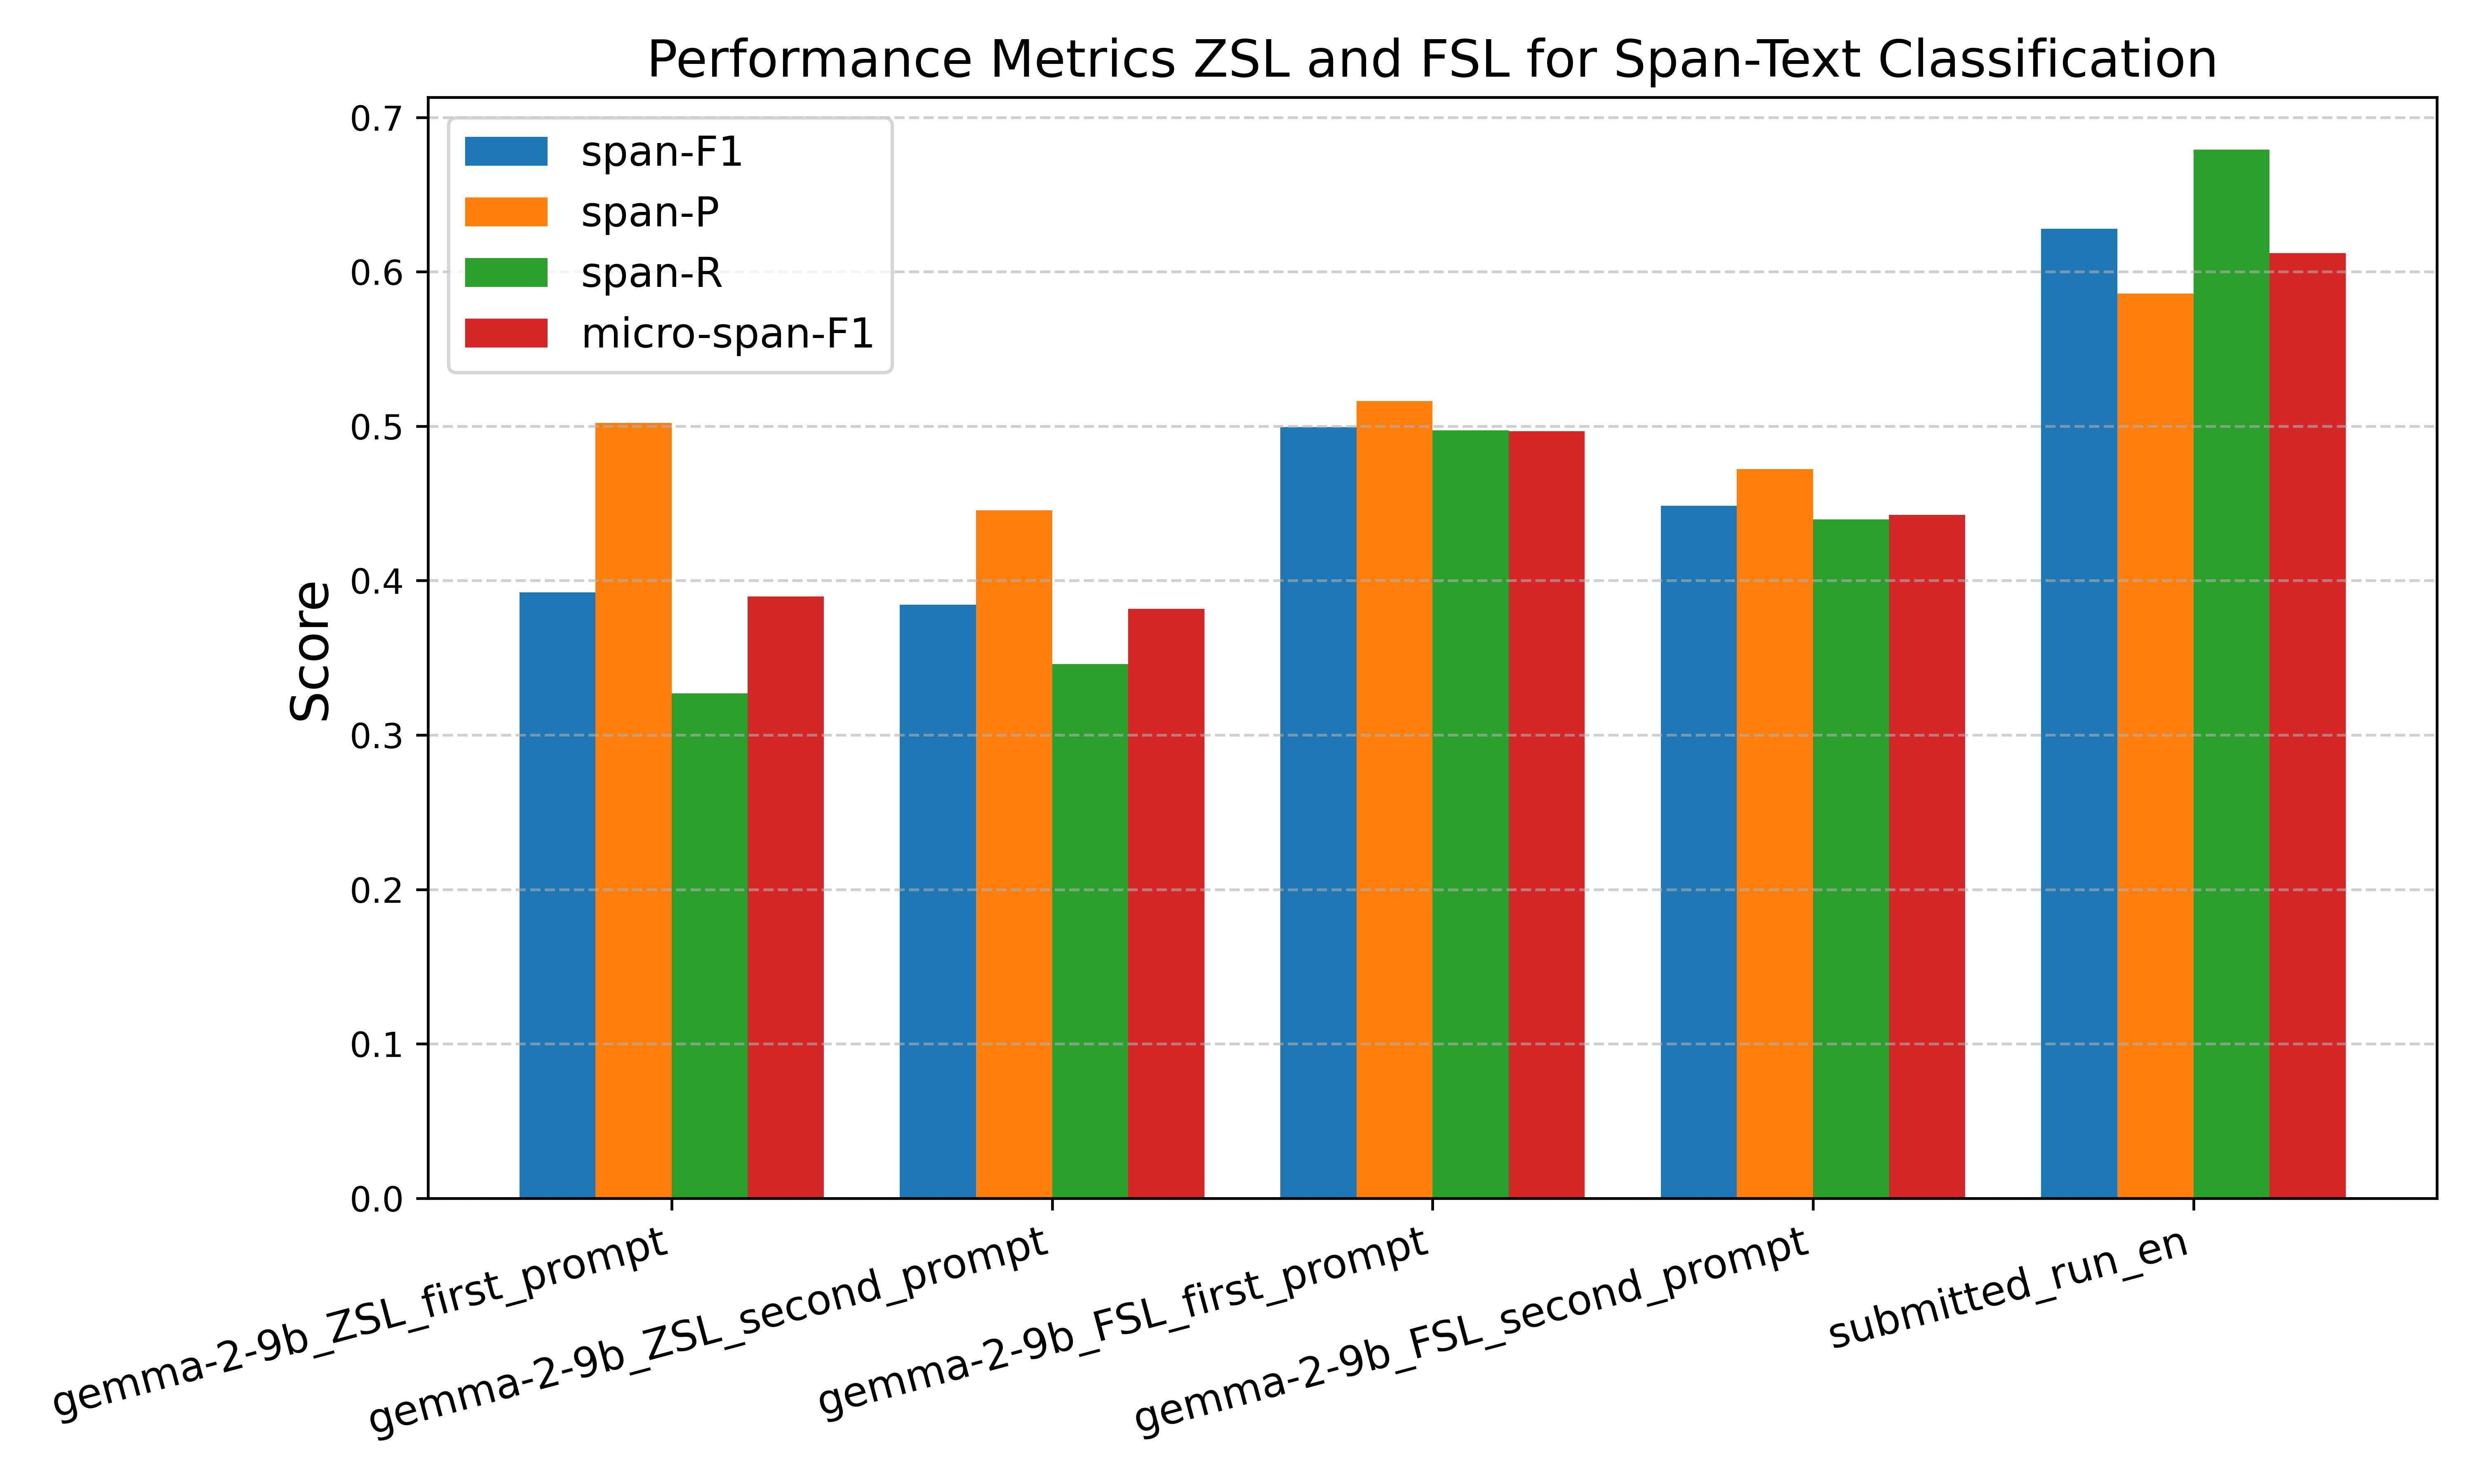
\includegraphics[width=0.95\linewidth, height=0.42\textheight]{Images/t2_zsl_fsl.png}
 \caption{Performance metrics of ZSL and FSL for span-text detection}
 \label{fig:t2_zsl_fsl}
\end{figure}
\FloatBarrier

\begin{table}[H]
\centering
\small
\renewcommand{\arraystretch}{1.2} % Increase row height
\begin{tabular}{lccccc}
\hline
\textbf{Model} & \textbf{Prompt} & \textbf{span-F1} & \textbf{span-P} & \textbf{span-R} & \textbf{micro-span-F1} \\
\hline
\multicolumn{6}{c}{\textbf{ZERO-SHOT}} \\
\hline
    gemma-2-9b-it  & first  &  \textbf{0.3923} & \textbf{0.5021} & 0.3269 & \textbf{0.3897} \\   
    gemma-2-9b-it  & second &  0.3843 & 0.4454 & \textbf{0.3459} & 0.3816 \\   
\hline
\multicolumn{6}{c}{\textbf{FEW-SHOT}} \\
\hline
    gemma-2-9b-it  & first & \textbf{0.4995} & \textbf{0.5162} & 0.4974 & \textbf{0.4968} \\   
    gemma-2-9b-it  & second & 0.4485 & 0.4723 & \textbf{0.4395} & 0.4426 \\   
\hline
\hline
\textit{submitted\_run} &  & \textit{0.6279} & \textit{0.5859} & \textit{0.6790} & \textit{0.6120}  \\
\hline
\end{tabular}
\caption{Performance metrics of ZSL and FSL for span-text detection}
\label{tab:performance_T2_ZSL_FSL}
\end{table}
\FloatBarrier


Analyzing Table \ref{tab:performance_T2_ZSL_FSL}, the micro-span-F1 metric clearly illustrates the impact of different learning strategies and prompt designs on the \textit{gemma-2-9b-it} model's performance. In the zero-shot learning setup, the first prompt, which provided detailed explanations, achieved a micro-span-F1 score of 0.3897. Although precision was relatively high at 0.5021, recall was significantly lower at 0.3269, indicating a tendency towards conservative predictions with many missed spans. The simplified second prompt slightly decreased micro-span-F1 to 0.3816, with precision dropping to 0.4454 but recall improving to 0.3459. This underscores the difficulty in balancing precision and recall without examples to guide the model.

The introduction of few-shot learning led to some improvements. The first FSL prompt increased micro-span-F1 to 0.4968, demonstrating how examples helped the model achieve a better balance between precision (0.5162) and recall (0.4974). Although the second FSL prompt also showed gains over ZSL, its micro-span-F1 was lower at 0.4426, revealing that a simpler prompt still limited the model's overall effectiveness.

Comparing these strategies, FSL had a clear advantage in boosting micro-span-F1, showing the importance of incorporating examples to enhance model confidence and generalization. Nevertheless, the \textit{submitted\_run} model outperformed all approaches, achieving a micro-span-F1 of 0.6120, with precision at 0.5859 and recall at 0.6790. This highlights the superiority of fine-tuning, which remains essential for maximizing both precision and recall. These findings emphasize that while prompt design and examples are beneficial, fine-tuning is crucial for achieving the highest performance in complex tasks.


\chapter{Conclusion and Future Work} \label{chap:conclusion_future_work}
In this thesis, we explored the detection of oppositional thinking narratives, specifically focusing on distinguishing between conspiratorial and critical thinking narratives and identifying narrative elements within texts. The research aimed to address the challenges of accurately classifying complex narrative structures using fine-tuned transformer models and LLMs, strategic data processing, data augmentation and ensemble methods. These techniques demonstrated the effectiveness of transformer-based approaches and LLMs approaches in handling nuanced language classification tasks, highlighting the models' adaptability, precision and potential for broader application across languages and domains.  

\section{Concluding Remarks}
This research has provided valuable insights by effectively addressing the three research questions and making significant contributions to the detection of oppositional narratives.

First, regarding the ability of transformer models and Large Language Models to distinguish between conspiracy theories and critical thinking narratives, the binary classification experiments confirmed that these models are highly effective. The combination of fine-tuned transformers, Large Language Models, and ensemble methods such as soft voting, led to high MCC scores, demonstrating robust performance in both English and Spanish datasets. This success underscores these models' capability to capture nuanced differences between conspiracy and critical thinking narratives, even when faced with the challenges of imbalanced datasets. The results validate both transformer-based models and LLMs as highly adaptable and precise in managing complex classification tasks across languages and narrative types, effectively distinguishing between these two forms of oppositional thought. 

Additionally, experiments with Large Language Models underscored the importance of task-specific fine-tuning. While zero-shot and few-shot learning approaches offered limited effectiveness, fine-tuning allowed the LLMs to achieve state-of-the-art performance, surpassing the initial systems submitted for the shared task. This outcome highlights the value of model-specific adaptations for optimal results in complex classification tasks. Similarly, experiments with multilingual transformer models confirmed the viability of a unified approach for processing both English and Spanish texts, validating the potential of multilingual binary classification for cross-lingual narrative analysis. These findings reinforce the significance of LLMs and multilingual transformer models in effectively distinguishing and classifying nuanced narratives across different languages and contexts.

Second, in terms of identifying and categorizing narrative elements within texts, this research demonstrated that it is feasible to detect and label key components such as Agents, Facilitators, Victims, Campaigners, Objectives, and Negative Effects within oppositional narratives. The span-level detection task posed notable complexity due to partially overlapping spans and the subtlety of narrative distinctions. However, strategic data preprocessing methods enabled the models to align tokens accurately, critical for precise span detection. Techniques like synonym replacement were essential for improving the models' generalization across linguistic variations without sacrificing precision. The use of multilingual transformer models played a pivotal role in this task, achieving high span-F1 scores across languages, thereby validating the models’ capacity for multilingual adaptability and fine-grained identification of narrative components across English and Spanish. This finding reinforces the significance of multilingual transformer models in effective narrative detection across diverse linguistic contexts.

Lastly, concerning the impact of data augmentation techniques on model performance, this thesis demonstrated that these techniques are essential for both binary classification and span-level detection. By addressing class imbalances and promoting generalization across linguistic variations, data augmentation improved MCC scores in binary classification, particularly aiding in the detection of underrepresented conspiracy texts. For span-level detection, augmentation techniques enabled models to handle diverse narrative structures effectively, underscoring their role in refining NLP models to capture the detailed structure of narratives.


\section{Future Works}
Building on the success of the span-level detection task, several promising directions for future research are evident. One key area is the integration of multimodal data, allowing models to process not only text but also images, videos, and audio. Disinformation often relies on non-textual content to amplify its impact, especially on platforms where visual media is prevalent. Extending models to handle multimodal content could enhance detection efforts, offering a more comprehensive understanding of narrative structures across various media.

Expanding these methods to low-resource languages is another important direction. Although this research achieved strong results in English and Spanish, the techniques can be adapted for languages with fewer resources. Cross-lingual transfer learning, where models trained on high-resource languages are adapted to low-resource ones, could significantly broaden the applicability of these models to address disinformation in regions particularly vulnerable to its effects.

Furthermore, the approaches are adaptable to other languages and domains, which allows for potential real-time applications such as monitoring social media to detect disinformation. However, deploying such systems raises ethical considerations around transparency and accountability to prevent misuse, emphasizing the need for responsible model deployment.

The narrative element detection framework could also benefit from exploring finer distinctions within the taxonomy of narrative elements. Although six fundamental elements were identified, future studies might analyze how narratives evolve over time or adapt to different contexts, enhancing the understanding of disinformation spread and informing more effective countermeasures.

Lastly, future research should focus on improving model interpretability. Although the models in this thesis performed well, their decision-making processes remain opaque. Techniques like LIME \cite{ribeiro2016model} or SHAP \cite{lundberg2017unified} could provide clearer insights into model predictions, an essential step for applications in high-stakes contexts such as content moderation or legal frameworks. Enhancing transparency will be key to ensuring these models are used ethically, responsibly, and effectively in broader applications.


%-------------------------------------------------------------------------
%	BIBLIOGRAPHY
%-------------------------------------------------------------------------

\addtocontents{toc}{\vspace{2em}} % Add a gap in the Contents, for aesthetics
%\bibliography{Thesis_bibliography} % The references information are stored in the file named "Thesis_bibliography.bib"
\begingroup
\footnotesize % you can also use \footnotesize or \scriptsize for even smaller fonts)
\bibliography{Thesis_bibliography} % The references information are stored in the file named "Thesis_bibliography.bib"
\endgroup

%-------------------------------------------------------------------------
%	APPENDICES
%-------------------------------------------------------------------------

\cleardoublepage
\addtocontents{toc}{\vspace{2em}} % Add a gap in the Contents, for aesthetics
\appendix

\chapter{Appendix B} \label{chap:appendix_B}
In this appendix, we provide the official rankings and performance metrics for Tasks 1 and 2 in both English and Spanish \cite{korencic2024oppositional}.

\section{Detailed Results for Task 1 in English}
In the following table (Table \ref{tab:task1_results_en_full}) are detailed the results and rankings of the teams participating on task 1, binary classification of text as either conspiracy or critical, for English texts. Performance metrics are: Matthews Correlation Coefficient, macro-averaged F1, and per-class binary F1’s.

\begin{table}[H]
\centering
\small
\renewcommand{\arraystretch}{0.8} % Reduce the space between rows
\begin{tabular}{clcccc}
\hline
\textbf{Pos.} & \textbf{Team} & \textbf{MCC} & \textbf{F1-Macro} & \textbf{F1-Conspiracy} & \textbf{F1-Critical} \\ \hline
1 & IUCL & 0.8388 & 0.9194 & 0.8947 & 0.9441 \\
2 & AI\_Fusion & 0.8303 & 0.9147 & 0.8866 & 0.9429 \\
3 & SINAI & 0.8297 & 0.9149 & 0.8886 & 0.9412 \\
4 & ezio & 0.8212 & 0.9097 & 0.8792 & 0.9402 \\
5 & hinlole & 0.8198 & 0.9098 & 0.8811 & 0.9386 \\
6 & Zleon & 0.8195 & 0.9096 & 0.8804 & 0.9388 \\
7 & virmel & 0.8192 & 0.9092 & 0.8793 & 0.9391 \\
8 & inaki & 0.8149 & 0.9072 & 0.8770 & 0.9374 \\
9 & yeste & 0.8124 & 0.9057 & 0.8746 & 0.9368 \\
10 & auxR & 0.8088 & 0.9043 & 0.8739 & 0.9347 \\
11 & Elias\&Sergio & 0.8034 & 0.9012 & 0.8687 & 0.9338 \\
12 & theateam & 0.8031 & 0.8999 & 0.8650 & 0.9347 \\
13 & trustno1 & 0.7983 & 0.8991 & 0.8675 & 0.9307 \\
14 & DSVS & 0.7970 & 0.8985 & 0.8674 & 0.9296 \\
15 & sail & 0.7969 & 0.8978 & 0.8687 & 0.9268 \\
16 & ojo-bes & 0.7969 & 0.8981 & 0.8648 & 0.9314 \\
17 & RD-IA-FUN & 0.7965 & 0.8977 & 0.8636 & 0.9317 \\
& \textit{baseline-BERT} & 0.7964 & 0.8975 & 0.8632 & 0.9318 \\
18 & aish\_team & 0.7917 & 0.8944 & 0.8580 & 0.9309 \\
19 & rfenthusiasts & 0.7902 & 0.8948 & 0.8605 & 0.9291 \\
20 & Dap\_upv & 0.7898 & 0.8944 & 0.8593 & 0.9294 \\
21 & oppositional\_opposition & 0.7894 & 0.8935 & 0.8571 & 0.9300 \\
22 & miqarn & 0.7881 & 0.8938 & 0.8593 & 0.9283 \\
\hline
\end{tabular}
\caption{\small Results for task 1 - English \cite{korencic2024oppositional}}
\label{tab:task1_results_en_full}
\end{table}
\FloatBarrier

\section{Detailed Results for Task 1 in Spanish}
In the following table (Table \ref{tab:task1_results_es_full}) are detailed the results and rankings of the teams participating on task 1, binary classification of text as either conspiracy or critical, for Spanish texts. Performance metrics are: Matthews Correlation Coefficient, macro-averaged F1, and per-class binary F1’s.

\begin{table}[H]
\centering
\small
\renewcommand{\arraystretch}{0.8} % Reduce the space between rows
\begin{tabular}{clcccc}
\hline
\textbf{Pos.} & \textbf{Team} & \textbf{MCC} & \textbf{F1-Macro} & \textbf{F1-Conspiracy} & \textbf{F1-Critical} \\ \hline
1 & SINAI & 0.7429 & 0.8705 & 0.8319 & 0.9091 \\
2 & auxR & 0.7205 & 0.8572 & 0.8112 & 0.9032 \\
3 & RD-IA-FUN & 0.7028 & 0.8497 & 0.8035 & 0.8960 \\
4 & Elias\&Sergio & 0.6971 & 0.8485 & 0.8087 & 0.8884 \\
5 & AI\_Fusion & 0.6872 & 0.8419 & 0.7931 & 0.8908 \\
6 & zhengqiaozeng & 0.6871 & 0.8417 & 0.7925 & 0.8909 \\
7 & virmel & 0.6854 & 0.8426 & 0.8022 & 0.8831 \\
8 & trustno1 & 0.6848 & 0.8400 & 0.7895 & 0.8906 \\
9 & Zleon & 0.6826 & 0.8410 & 0.7955 & 0.8865 \\
10 & ojo-bes & 0.6817 & 0.8395 & 0.8026 & 0.8764 \\
11 & tulbure & 0.6722 & 0.8293 & 0.7699 & 0.8887 \\
12 & sail & 0.6719 & 0.8299 & 0.7713 & 0.8884 \\
13 & nlpln & 0.6681 & 0.8339 & 0.7872 & 0.8806 \\
& \textit{baseline-BETO} & 0.6681 & 0.8339 & 0.7872 & 0.8806 \\
14 & pistacchio & 0.6678 & 0.8327 & 0.7822 & 0.8833 \\
15 & rfenthusiasts & 0.6656 & 0.8255 & 0.7643 & 0.8868 \\
16 & XplaiNLP & 0.6622 & 0.8274 & 0.7708 & 0.8840 \\
17 & yeste & 0.6609 & 0.8291 & 0.7770 & 0.8812 \\
18 & oppositional\_opposition & 0.6601 & 0.8274 & 0.7724 & 0.8825 \\
19 & epistemologos & 0.6562 & 0.8264 & 0.7728 & 0.8801 \\
20 & miqarn & 0.6562 & 0.8264 & 0.7728 & 0.8801 \\
\hline
\end{tabular}
\caption{\small Results for task 1 - Spanish \cite{korencic2024oppositional}}
\label{tab:task1_results_es_full}
\end{table}


\section{Detailed Results for Task 2 in English}
In the following table (Table \ref{tab:task2_results_en_full}) are detailed the results and rankings of the teams participating on task 2, token classification of span-level narrative elements, for English texts. The performance metrics are: span-F1 (macro-averaged over span labels), span-precision, span-recall, and micro-averaged span-F1. 

\begin{table}[H]
\centering
\small
\renewcommand{\arraystretch}{0.8} % Reduce the space between rows
\begin{tabular}{clcccc}
\hline
\textbf{Position} & \textbf{Team} & \textbf{span-F1} & \textbf{span-P} & \textbf{span-R} & \textbf{micro-span-F1} \\ \hline
1 & tulbure & 0.6279 & 0.5859 & 0.6790 & 0.6120 \\
2 & Zleon & 0.6089 & 0.5537 & 0.6881 & 0.5856 \\
3 & hinlole & 0.5886 & 0.5243 & 0.6834 & 0.5571 \\
4 & oppositional\_opposition & 0.5866 & 0.5347 & 0.6586 & 0.5344 \\
5 & AI\_Fusion & 0.5805 & 0.5585 & 0.6082 & 0.5437 \\
6 & virmel & 0.5742 & 0.5235 & 0.6477 & 0.5540 \\
7 & miqarn & 0.5739 & 0.5184 & 0.6462 & 0.5325 \\
8 & TargaMarhuenda & 0.5701 & 0.5161 & 0.6477 & 0.5437 \\
9 & ezio & 0.5694 & 0.5229 & 0.6340 & 0.5389 \\
10 & zhengqiaozeng & 0.5666 & 0.5122 & 0.6485 & 0.5421 \\
11 & Elias\&Sergio & 0.5627 & 0.5149 & 0.6364 & 0.5248 \\
12 & DSVS & 0.5598 & 0.5332 & 0.6012 & 0.5287 \\
13 & CHEEXIST & 0.5524 & 0.4767 & 0.6845 & 0.5299 \\
14 & rfenthusiasts & 0.5479 & 0.5381 & 0.5666 & 0.5408 \\
15 & ALC-UPV-JD-2 & 0.5377 & 0.4643 & 0.6562 & 0.4956 \\
& \textit{baseline-BERT} & 0.5323 & 0.4684 & 0.6334 & 0.4998 \\
16 & Dap\_upv & 0.5272 & 0.4617 & 0.6297 & 0.4973 \\
17 & aish\_team & 0.5213 & 0.4181 & 0.7456 & 0.2571 \\
18 & SINAI & 0.4582 & 0.5553 & 0.4279 & 0.4571 \\
19 & Trainers & 0.3382 & 0.5124 & 0.2609 & 0.2858 \\
20 & nlpln & 0.3339 & 0.5286 & 0.3303 & 0.2710 \\
21 & ROCurve & 0.2996 & 0.3154 & 0.3031 & 0.3425 \\
22 & TokoAI & 0.2760 & 0.1870 & 0.6119 & 0.2677 \\
23 & DiTana & 0.2756 & 0.5259 & 0.1947 & 0.2599 \\

\hline
\end{tabular}
\caption{\small Results for task 2 - English \cite{korencic2024oppositional}}
\label{tab:task2_results_en_full}
\end{table}
\FloatBarrier

\begin{table}[H]
\ContinuedFloat
\centering
\small
\renewcommand{\arraystretch}{0.8} % Reduce the space between rows
\begin{tabular}{clcccc}
\hline
\textbf{Position} & \textbf{Team} & \textbf{span-F1} & \textbf{span-P} & \textbf{span-R} & \textbf{micro-span-F1} \\ \hline
24 & TheGymNerds & 0.2070 & 0.2076 & 0.2127 & 0.2329 \\
25 & epistemologos & 0.1709 & 0.1286 & 0.3244 & 0.1201 \\
25 & epistemologos & 0.1709 & 0.1286 & 0.3244 & 0.1201 \\
26 & theateam & 0.1503 & 0.1401 & 0.1652 & 0.0387 \\
27 & LaDolceVita & 0.0726 & 0.2040 & 0.0453 & 0.0630 \\
28 & kaprov & 0.0150 & 0.0261 & 0.0165 & 0.0600 \\
\hline
\end{tabular}
\caption{Results for task 2 - English (cont.) \cite{korencic2024oppositional}}
\label{tab:task2_results_en_full}
\end{table}
\FloatBarrier

\section{Detailed Results for Task 2 in Spanish}
In the following table (Table \ref{tab:task2_results_es_full}) are detailed the results and rankings of the teams participating on task 2, token classification of span-level narrative elements, for Spanish texts. The performance metrics are: span-F1 (macro-averaged over span labels), span-precision, span-recall, and micro-averaged span-F1.

\begin{table}[H]
\small
\renewcommand{\arraystretch}{0.8} % Reduce the space between rows
\begin{tabular}{clcccc}
\hline
\textbf{Position} & \textbf{Team} & \textbf{span-F1} & \textbf{span-P} & \textbf{span-R} & \textbf{micro-span-F1} \\ \hline
1 & tulbure & 0.6129 & 0.6159 & 0.6129 & 0.6108 \\
2 & Zleon & 0.5875 & 0.5439 & 0.6474 & 0.5939 \\
3 & AI\_Fusion & 0.5777 & 0.5437 & 0.6189 & 0.5843 \\
4 & CHEEXIST & 0.5621 & 0.5379 & 0.5995 & 0.5456 \\
5 & virmel & 0.5616 & 0.4963 & 0.6584 & 0.5620 \\
6 & miqarn & 0.5603 & 0.5117 & 0.6273 & 0.5618 \\
7 & DSVS & 0.5529 & 0.5384 & 0.5785 & 0.5323 \\
8 & TargaMarhuenda & 0.5364 & 0.5128 & 0.5710 & 0.5385 \\
9 & Elias\&Sergio & 0.5151 & 0.4864 & 0.5533 & 0.5231 \\
10 & hinlole & 0.4994 & 0.4530 & 0.5740 & 0.4890 \\
& \textit{baseline-BETO} & 0.4934 & 0.4533 & 0.5621 & 0.4952 \\
11 & Dap\_upv & 0.4914 & 0.4555 & 0.5474 & 0.4917 \\
12 & zhengqiaozeng & 0.4903 & 0.4507 & 0.5494 & 0.4874 \\
13 & ALC-UPV-JD-2 & 0.4885 & 0.4509 & 0.5458 & 0.4683 \\
14 & ezio & 0.4869 & 0.4623 & 0.5229 & 0.4947 \\
15 & nlpln & 0.4672 & 0.5174 & 0.4426 & 0.2961 \\
16 & rfenthusiasts & 0.4666 & 0.5104 & 0.4341 & 0.4697 \\
17 & SINAI & 0.4151 & 0.4630 & 0.4054 & 0.4781 \\
18 & TheGymNerds & 0.3984 & 0.3621 & 0.4483 & 0.5024 \\
19 & DiTana & 0.3004 & 0.4490 & 0.2362 & 0.3117 \\
20 & ROCurve & 0.2649 & 0.2706 & 0.2627 & 0.3562 \\
21 & TokoAI & 0.1878 & 0.1189 & 0.5659 & 0.1739 \\
22 & epistemologos & 0.1657 & 0.1906 & 0.1864 & 0.1534 \\
23 & LaDolceVita & 0.1056 & 0.1158 & 0.0975 & 0.1321 \\
24 & theateam & 0.0994 & 0.1051 & 0.0962 & 0.0358 \\
25 & oppositional\_opposition & 0.0037 & 0.0349 & 0.0022 & 0.0014 \\
\hline
\end{tabular}
\caption{\small Results for task 2 - Spanish \cite{korencic2024oppositional}}
\label{tab:task2_results_es_full}
\end{table}
\FloatBarrier


% LIST OF FIGURES
\listoffigures

% LIST OF TABLES
\listoftables

\begin{comment}
% LIST OF SYMBOLS
% Write out the List of Symbols in this page
\chapter*{List of Symbols} % You have to include a chapter for your list of symbols (
\begin{table}[H]
    \centering
    \begin{tabular}{lll}
        \textbf{Variable} & \textbf{Description} & \textbf{SI unit} \\\hline\\[-9px]
        $\bm{u}$ & solid displacement & m \\[2px]
        $\bm{u}_f$ & fluid displacement & m \\[2px]
    \end{tabular}
\end{table}
\end{comment}


\cleardoublepage

\end{document}
